%%===================================
% === MAIN-file =====================
% This template is made by Oda Lauten
%%===================================
\documentclass[12pt, a4paper, twoside, openright]{book}
\usepackage{config/packages}
\usepackage{config/commands}
\usepackage{config/input}
\usepackage{frontmatter/acronyms}
\begin{document}

%\tracingall  %  will print some additional error messages in some cases.

%%===================================
% --- Frontmatter
%%===================================
\frontmatter

\begin{comment}

% Title page
%%=========================================
\begin{titlepage}
\parindent=0.0cm
\parskip = 1.0ex
    \begin{center}
        \vspace*{1.0cm}
        \Huge {\title}\\
        %\vspace{0.5cm}
        %{\Large {\subtitle}}\\
        \vspace{2.0cm}
        {\LARGE {\emph{\author}}}
        
        \vfill
                
        \includegraphics[width=0.2\textwidth]{ntnu_logo.png}
        
        \Large
        \vspace{2.0cm}
        \department     \\
        \vspace{0.02cm}
        \faculty        \\
        \vspace{0.02cm}
        \university     \\
        
        \vspace{1.0cm}
        \textbf{\month~\year}\\
        
        
        \vspace{0.5cm}
    
    \end{center}
\end{titlepage}
%%=========================================


% Information
%%=========================================
\clearpage
\thispagestyle{empty}
{~}
\vfill
{
\scriptsize
\textbf{\univ}

\university

\department \\
\faculty

\author: \textit{\title}, \month~\year

Supervisors:\\
\supervisorFFI, \supervisorFFILocation\\
\supervisorNTNU, \supervisorNTNULocation

Location:\\
\location

%\textcopyright~\year~\author. All rights reserved.

%ISBN <<ISBN PRINTED VERSION>>\ (printed version)\\
%ISBN <<ISBN ELECTRONIC VERSION>>\ (electronic version)\\
%ISSN 1503-8181

%Master thesis at \univ, <<SERIAL NUMBER>>

Printed by \printedby
}
%%=========================================

% Preface [optional]
%%=========================================
\chapter*{Preface}%\addcontentsline{toc}{chapter}{Preface}
% Here you give a brief introduction to your work. What it is (e.g. a Master's thesis in RAMS at NTNU as a part of the study program XXX and ...) and when it was carried out (e.g. during the autumn of semester of 2021). If it was carried out for a company, you should mention this and also describe the cooperation with the company. You may also describe how the idea to the project was brought up.
%
This master's thesis is submitted as the final work required for the Master's degree (MSc) in Applied Physics and Mathematics at the Norwegian University of Science and Technology (NTNU). The study presented in this thesis was carried out at the Norwegian Defence Research Establishment (FFI) from January to June 2017 under the supervision of Professor Randi Haakenaasen. 

The study is a continuation of the Specialization Project in Physics (TFY4510, 15 ECTS), as presented in the author's report titled \inquote{Characterisation of As-Received \ce{CdZnTe} Substrates} \citep{lauten2017characterisation}. Some of the results are reiterated here in order to better present the full scope of the study that has been performed during the final year of my MSc studies. %which involved a characterization of two as-received \ce{CdZnTe} substrates from different vendors

% The thesis is to some extent built on previously obtained results, as presented in the author’s project work titled ’Precipitation of Several Coexisting Strengthening Phases in Aluminium Alloys’, written during the autumn of 2015. Some of the contents in this project work are re-given here, in order to better present the full scope of scientific work performed during the final year of my MSc studies in applied physics and mathematics. The thesis serves a dual purpose; studying the multiphase nature of 2xxx series Al alloys, as well as providing an introduction to the SPED technique. It is intended for readers who are interested with one or both of these topics.
%
%\subsection*{Acknowledgments}
%First of all
I would like to thank Professor Randi Haakenaasen for giving me the possibility to carry out the work presented in this thesis. I am grateful for the valuable discussions and guidance during my work. I would also like to thank Chief Scientist Espen Selvig at FFI for his patient advice and follow up in the development of this work; Senior Scientist Kjell Ove Kongshaug and Technician Laila Trosdahl-Iversen at FFI for demonstrating the preparation methods used before epitaxial growth; and Senior Engineer Torgeir Lorentzen at FFI for giving me training at the atomic force microscope and for generally being helpful in practical matters.
%
%Associate Professor Turid Worren Reenaas at NTNU for taking the time to read my master's thesis and provide useful feedback; 
%%=========================================

\vspace{1.0cm}
\begin{flushright}
Oda Lauten      \\
Kjeller, Norway \\
\month~\year      \\
\end{flushright}

%%=========================================

% Dedication [optional]
%%%=========================================
\clearpage
\thispagestyle{empty}
\null\vspace{\stretch{1}}
\begin{flushright}
\textit{Dedicated to Google and Wikipedia\\for their love, endless support\\and encouragement.}
\end{flushright}
\null\vspace{\stretch{3}}\null
%%=========================================

% Abstract
%%=========================================
% Here you give a summary of your work and your results. This is like a management summary and should be written in a clear and easy language, without many difficult terms and without abbreviations. Everything you present here must be treated in more detail in the main report. You should not give any references to the report in the summary - just explain what you have done and what you have found out. Should NOT be more than two pages!
%%=========================================
\cleardoublepage  % to get the abstract to start on an odd page (right-hand page)
\selectlanguage{english}
\begin{abstract}
In this study, three different \ac{czt} substrates were characterised for surface impurity contamination, particles, and defects. The substrates were examined both as-received and after surface pre-growth preparation. As the final step, a layer of \ac{mct} film was grown on each substrate and examined. It is of great interest to obtain a better understanding of how impurities, defects, and particles on the \ac{czt} substrate surface affect the quality of the grown \ac{mct} film.  %%The \ac{mct} film is used to fabricate high performance photovoltaic \ac{ir} detectors. It is important to grow films with high crystallinity, i.e. few grain boundaries and almost no dislocations, and few defects and impurities to ensure that the detector elements that are processed on the film function properly. Hence, i

Two of the substrates were (111)B-oriented and used for \ac{lpe} growth of \ac{mct}: substrate A from vendor A, generally recognised to fabricate the best \ac{czt} substrates, and substrate B from vendor B, which was compared to vendor A. One additional substrate from vendor B, substrate B2, was studied as well. The last substrate was (211)B-oriented and used for \ac{mbe} growth of \ac{mct}, substrate C from vendor A.  The characterisation consisted of a study by optical microscopy, \ac{sem} with \ac{eds}, \ac{afm}, near-\ac{ir} transmission microscopy, and \ac{ftir}. 
%Three $30\times$\SI{30}{\milli\metre^2} (111)B-oriented substrates from two different vendors and one $15\times$\SI{15}{\milli\metre^2} (211)B-oriented substrate 
%The substrates were then subjected to different surface pre-growth preparations. The third $30\times$\SI{30}{\milli\metre^2} (111)B-oriented substrate was a replacement for the second substrate, which broke during this characterisation step. %The state-of-the-art (111)B-oriented substrate was subjected to \ac{lpe} preparation etch, the (111)B-oriented substrates were subjected to \ac{lpe} preparation polish and etch, while the state-of-the-art (211)B-oriented substrate was subjected to \ac{mbe} preparation etch.

The as-received substrate A had the best surface polish and crystal quality and had almost no particles on the surface. Surprisingly, the preparation etch procedure introduced more particles on the surface. The as-received substrate B had scratches, particles, and voids on the surface, and it had a larger surface roughness than the as-received substrate A by a factor of 10. The roughness decreased after the polishing procedure to about the same value as substrate A. The number of particles also decreased, but it was not as low as on substrate A. While the as-received substrate A had a density of polishing grit less than \SI{2e4}{\centi\metre^{-2}}, the as-received substrate C had an average density of \SI{4e7}{\centi\metre^{-2}}. The polishing grit density was reduced by a factor of 10 after etch.%Furthermore, the voids were indicative of poorer crystal quality than substrate A. The results from the polished substrate B was reproduced on the polished substrate B2.

The surface of the \ac{mct} epilayers that were grown by \ac{lpe} on substrate A and substrate B2 showed wavy structures on the surface with doughnut-shaped defects and large circular defects with a density of \SIrange{1e4}{2e4}{\centi\metre^{-2}} and \SI{\sim 2}{\centi\metre^{-2}} respectively. The doughnut-shaped defects seemed to correlate with the polishing grit on substrate B2, but showed no correlation with the polishing grit on substrate A. The \ac{mct} epilayer that was grown by \ac{mbe} on substrate C had a microvoid density of \SI{1e+05}{\centi\metre^{-2}}, which correlated with polishing grit observed before growth.

\end{abstract}
%%=========================================

%%=========================================
\cleardoublepage  % to get the abstract to start on an odd page (right-hand page)
\selectlanguage{norsk}
\begin{abstract}

I dette studiet ble tre ulike \acf{czt} substrater karakterisert for urenheter, partikler og defekter. Substratene ble karakterisert både som motatt fra leverandør og etter forbehandling før groing. Til slutt ble det grodd ett lag med \acf{mct} film på hvert av substratene og filmen ble karakterisert. Det er av interesse å få en bedre forståelse av hvordan urenheter, defekter og partikler på overflaten av substratet påvirker kvaliteten på den grodde \ac{mct} filmen. %\Ac{mct}-filmer blir brukt til å produsere infrarøde (IR) detektorer med høy ytelse.

To av substratene var (111)B-orienterte og brukt til å gro \ac{mct} ved væskefaseepitaksi (LPE): substrat A fra leverandør A, kjent for å produsere substrater av ypperste kvalitet, og substrat B leverandør A, som ble sammenlignet med leverandør A. Ett ekstra substrat fra leverandør B, substrat B2, ble også studert. Det siste substratet var (211)B-orientert og brukt til å gro \ac{mct} ved molekylstråleepitaksi (MBE), substrat C fra leverandør A. Karakteriseringen ble gjennomført ved bruk av optisk mikroskop, sveipeelektronmikroskop (SEM), energidispersiv røntgenspektroskopi (EDS), atomærkraftmikroskopi (AFM), nær-IR transmisjonsmikroskopi og Fouriertransform infrarød spektroskopi (FTIR).

Substrat A hadde den beste overflatepoleringen og krystallkvaliteten som motatt fra leverandør, og hadde omtrent ingen partikler på overflaten. Overraskende nok hadde substrat A mer partikler på overflaten etter etseprosedyren. Substrat B hadde riper, partikler og hulrom på overflaten, og overflateruheten var 10 ganger større enn for substrat A som motatt. Ruheten minket til omtrent det samme som substrat A etter polering og etsing. Antall partikler minket også, men ble ikke like lavt som for substrat A. Substrat C hadde en gjennomsnittlig tetthet at poleringspartikler på \SI{4e7}{\centi\metre^{-2}} som motatt fra leverandør i motsetning til substrat A som hadde en poleringspartikkeltetthet mindre enn \SI{2e4}{\centi\metre^{-2}} som motatt fra leverandør. Tettheten ble redusert med en faktor 10 etter etsing. %Hulrommene i overflaten antyder at krystallkvaliteten var dårligere enn for substrat A. Resulatet for det polerte substrat B ble reprodusert for the polerte substrat B2. 

Overflaten på de LPE-grodde lagene viste en bølgete struktur typisk for LPE med smultringformede defekter og større sirkulære defekter med en tetthet på henholdsvis \SIrange{1e4}{2e4}{\centi\metre^{-2}} og \SI{\sim 2}{\centi\metre^{-2}}. De smultringformede defektene så ut til å korrelere med poleringspartikler på substrat B2, men viste ingen korrelasjon med poleringspartikler på substrat A. \Ac{mct} filmen som ble grodd på substrat C hadde en tetthet av mikrohulrom på \SI{1e+05}{\centi\metre^{-2}}. Mikrohulrommene korrelerte med partikler observert på overflaten av substratet før groing.

\end{abstract}
%%=========================================
\selectlanguage{english}
%%=========================================

% Acknowledgements [optional]
%%%=========================================
\renewcommand{\abstractname}{Acknowledgements}
\begin{abstract}
I would like to thank my supervisor Professor Randi Haakenaasen for the valuable discussions and guidance during my project work. I would also like to thank my professors at NTNU for their inspiring lectures and discussions, and my co-supervisor Associate Professor Turid Worren Reenaas for making time for me in her already busy schedule.

The work has been carried out in co-operation with the Norwegian Defence Research Establishment (FFI) at Kjeller. I would like to thank Espen Selvig for his patient advice and follow up in the development of this work, Laila Trosdahl-Iversen for useful guidance during transfer of samples, and Torgeir Lorentzen for helping me when the machines did not work properly.
\end{abstract}
%%=========================================
%% E.g. I would like to thank the following persons for their great help during... 
%% If the project has been carried out in cooperation with an external partner (i.e. a company), you should acknowledge the contribution and give thanks to the involved persons. You should also acknowledge the contributions made by your supervisor(s).

% Quote [optional]
%%%=========================================
\cleardoublepage  % to get the abstract to start on an odd page (right-hand page)
\vspace*{\fill} 
\begin{quote} 
\begin{center} 
\textit{``Neque porro quisquam est qui dolorem ipsum quia dolor sit amet, consectetur, adipisci velit.''}\\ % ``Neither is there anyone who loves, pursues or desires pain itself because it is pain.''
\hfill (Cicero, 45 BC.)
\end{center}
\end{quote}
\vspace*{\fill}
%%=========================================

% Table of Contents
\renewcommand*\contentsname{Table of Contents}
\tableofcontents

% List of figures [optional]
\listoffigures

% List of tables [optional]
\listoftables

% List of acronyms and abbreviations (symbols, and notation) [optional]
\printacronyms[heading=chapter, name=List of Acronyms, include-classes = {acro}, sort=true]

\end{comment}


%%===================================
% --- Mainmatter
%%===================================
\mainmatter

% Resets acronyms.
% Each acronym will behave as if it is called for the first time.
\acresetall

% Chapters
%%%=========================================
\chapter{Introduction}
%This chapter gives an introduction to the use of \ac{czt} substrates to grow \ac{mct} films for \ac{ir} detectors. Then literature survey, problem formulation, and structure of the report.
% The first chapter of a well-structured thesis is always an introduction, setting the scene with background, problem description, objectives, limitations, and then looking ahead to summarise what is in the rest of the report. This is the part that readers look at first—so make sure it hooks them!

%\Ac{czt} is a substrate for epitaxial growth of lattice-matched \ac{mct} films used for infrared detectors. 

%Roughness, oxidation, defects, or contamination on the \ac{czt} surface can affect the growth of \ce{CdHgTe}. Hence, smooth and defect free surfaces are necessary to obtain high performance \ac{mct} infrared detectors.

%Chemo-mechanical polishing is used to obtain a smooth and planar surface. Both substrates are chemically etched in a bromine-methanol (\ce{Br-MeOH}) solution to remove the fine scratches that result from the chemo-mechanical polishing and the \ce{TeO2} layer that forms as the substrate is exposed to air.

The semiconducting material \ac{mct} is used to produce \acp{irfpa} for imaging of objects in the \ac{ir} region. The \ac{irfpa} consists of a 2-dimensional array of \ac{ir} detector elements at the focal plane of a lens. When an \ac{ir} photon with energy greater than the band gap is absorbed by the detector element, an electron will be excited from the valence band and placed in the conduction band. The charge, which is proportional to the number of absorbed photons, is collected at each detector element and converted to voltage by a \ac{roic} before the voltage signal is transferred to off-chip electronics. The measured signal from each detector element determine the intensity at the corresponding image pixel. The highest sensitivity \ac{mct} detector material is grown on lattice matched \ac{czt} substrates \citep{benson2016analysis}.
%An \ac{irfpa} operate by generating an electrical charge in relation to the number of photons that are detected at each pixel. 
%Electrical current, integrated decides the intensity of pixel. Pin hole/optics to make only photons from scenery if interest detected. 

%%=========================================
\section{Background}%\todo{Må skrive om denne seksjonen.}
% In this section, you should present the problem that you are going to investigate or analyze; why this problem is of interest; what has, so far, been done to solve the problem, and which parts of the problem that remain.

What makes the semiconducting material \ac{mct} suitable for \ac{ir} detectors, is the fact that it has high absorption, excellent lattice match with \ac{czt} substrates, and a tunable band gap which covers the entire \ac{ir} region from \SI{-0.26}{\electronvolt} to \SI{1.61}{\electronvolt} at \SI{77}{\kelvin} \citep{hansen1982energy}. Hence, the material can be adapted to detect \ac{ir} radiation in any of the \ac{ir} atmospheric transmission windows. The atmospheric transmission windows refer to the wavelength regions in which there is little absorption in the atmosphere: \ac{lwir} from \SI{8}{\micro\metre} to \SI{13}{\micro\metre}, \ac{mwir} from \SI{3}{\micro\metre} to \SI{5}{\micro\metre}, and \ac{swir} from \SI{1}{\micro\metre} to \SI{3}{\micro\metre}. An example of the atmospheric transmittance through 1 nautical mile, i.e. \SI{1.9}{\kilo\metre}, following a path at sea level can be seen in Fig.~\ref{fig:atm_window}. \Ac{ir} detection systems are usually designed to operate in these windows, so that radiation emitted from targets of interest can pass through the intermediate atmosphere and reach the detection system.
%to the transparent wavelength regions of the atmosphere. In the infrared region of the electromagnetic transmission spectra there can be seen an atmospheric window in the \ac{lwir}, that covers the wavelength range from \SI{8}{\micro\metre} to \SI{13}{\micro\metre}, and a fragmented atmospheric window can be observed in the \ac{swir} and \ac{mwir}, that covers the wavelength range from \SI{1}{\micro\metre} to \SI{3}{\micro\metre} and \SI{3}{\micro\metre} to \SI{5}{\micro\metre} respectively, see Fig.~\ref{fig:atm_window}.

\begin{figure}[htbp]
    \centering
    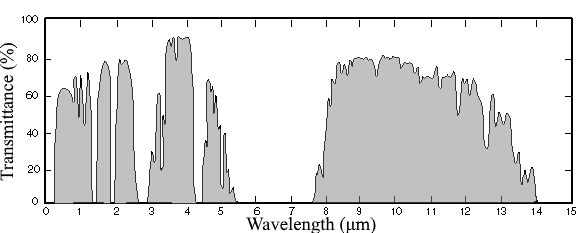
\includegraphics[width=0.8\columnwidth]{atmosfaerisk_spredning}
    \caption[Atmospheric transmittance versus wavelength.]{Atmospheric transmittance versus wavelength through 1 nautical mile (\SI{1.9}{\kilo\metre}) following a path at sea level. The transmittance is given in percent of total incoming radiation. A transmission window can be seen in the \acf{lwir} for wavelengths between \SI{8}{\micro\metre} and \SI{13}{\micro\metre} and a fragmented transmission window can be seen in the \acf{swir} and \acf{mwir} for wavelengths between \SI{0.2}{\micro\metre} and \SI{5}{\micro\metre}. The molecules mainly responsible for absorption are \ce{H2O}, \ce{CO2} and \ce{O2}. Modified from \citet{naval2013electronic}.}
    \label{fig:atm_window}
\end{figure}
%\mycomment{Indiker gjerne med piler, srkavering, sirkler eller på annen måte de vinsuene du har nevnt i teksten.}

The infrared detector applications of \ac{mct} and its consequential military role has made it a highly researched material, and it is used to make infrared detectors with high performance. In recent years, the technology has been increasingly utilised in many commercial products, e.g. medical diagnostics, drivers' enhanced vision, security applications and machine vision \citep{dhar2013advances}.
%Et materiale er vel ikke et forskningsfelt?  Materialet er interessant på grunn av egenskapene og de mulige anvendelsene, og det forskes på utvikling av ???  Framstillingsmetoder, materialegenskeper, anvendelser...?

\subsection{The Epitek Laboratory}

The Epitek laboratory at the \ac{ffi} is a laboratory for research on semiconducting materials. The main research focus is on growth of \ac{mct}, which is used in production of infrared detectors. This research consists of developing techniques and technologies for processing and characterising of both materials and components.

At the Epitek laboratory, \ac{czt} is used as a substrate material for both \ac{mbe} and \ac{lpe} growth of \ac{mct}. Epitaxy refers to the growth of a crystalline layer with a well-defined orientation determined by the crystal structure of the substrate. Defects, dislocations, impurities, and particles in and on the substrate will affect the growth and quality of the thin film layer. In the worst-case scenario, the processed \ac{ir} detector element will be defective due to the use of a poor \ac{mct} material. %in such a way that it becomes degraded, which in turn the processed \ac{ir} detector element defective.

The motivation for this study is the desire to obtain a better understanding of how impurities and defects on the \ac{czt} substrate surface affect the quality of the \ac{mct} films grown on the substrates. A long and tedious preparation process is required to get satisfying substrate surface quality for epitaxial growth \citep{triboulet2009cdteI}. Since the \ac{mct} detector material is grown directly on the \ac{czt} substrate, the as-received surface and the following pre-growth preparation of the surface are critical in the production of high quality detector material \citep{benson2015as-received}. It is important to grow films with high crystallinity, i.e. few grain boundaries and almost no dislocations, and few defects and impurities to ensure that the detector elements that are processed on the film function properly.

%%=========================================
\section{Literature Survey}%\todo{Må skrive om denne seksjonen.}
% You should here present the main books and articles that treat problems that are similar to what you are studying. If you, later in your thesis, describe the “state of the art” – with a detailed literature survey, you may just give a very brief survey here (approx. a quarter of a page). If this is the only literature survey, you need to go into more details. An objective of the literature survey is to show the reader that you are familiar with the main literature within your field of research – so that you do not “reinvent the wheel.”
%
% References to literature can be given in two different ways: 
% • As an explicit reference: It is shown by Lundteigen and Rausand (2008) and partly also by Rausand and Høyland (2004) that ...
% • As an implicit reference: It is shown (e.g., see Rausand and Høyland, 2004, Chap. 4) that ...
%
% In the example above, we have used “author-year” references, which is the preferred format.
%
% Remark: Following agreement with your supervisor, you may also refer by numbers, for example, [1]. 
%
% When you refer to the scientific literature, you should always write in present tense. Example: Rausand and Høyland (2004) show that ...
%
Defects in \ac{mbe}-grown \ac{mct} have been studied by many groups. \citet{selvig2007defects, selvig2008defects-a, selvig2008defects-b} at \ac{ffi} have described these defects as microvoids, hillocks, high temperature voids, needles, and dislocations. Microvoids are formed during growth at low substrate temperatures and can start at a defect or particle at the substrate surface. High temperature voids appear at higher temperatures, when \ce{Hg} evaporates from the film and leaves an excess of \ce{Te} which then collects in high temperature voids along with some polycrystalline \ce{CdTe} and \ac{mct}. The temperature where this occurs is called the tellurium phase limit.

A study of the impact of precipitates and contamination in \ac{czt} substrates on growth of \ac{mct} has been conducted by \citet{benson2014impact, benson2015as-received, benson2016analysis}. They studied state-of-the-art (211)B oriented \ac{czt} substrates for growth of \ac{mct} by \ac{mbe}. They associated two categories of \ac{mct} defects with defects originating in the substrate surface. The first was high temperature voids and bumps on the surface of \ac{mct} that were a result of tellurium precipitates in the underlying \ac{czt} substrate. The second was microvoid defects in the \ac{mct} film that originated in pits on the substrate surface. Their study of contamination on the as-received \ac{czt} substrates revealed polishing scratches,  residual polishing grit, \ce{Te} precipitates, \ce{Te} inclusions, \ac{czt} particles, and mounting wax. They observed that the residual polishing grit and mounting wax was removed by etching, but that the surface contamination of \ac{czt} particles was not removed by a standard \ac{mbe} preparation etch. %% substrates were from vendor A

%%=========================================
\section{Problem Formulation}%\todo{Må skrive om denne seksjonen.}
% You should define your problem in a clear an unambiguous way and explain why this is a problem, why it is of interest—and to whom. It is also important to delimit the problem area.
% OPPGAVEBESKRIVELSEN: Vi gror HgCdTe tynne filmer på \ac{czt} substrater. For å gro godt materiale, dvs med få defekter og dislokasjoner som kan degradere eller helt ødelegge et detektorelement, er det viktig at substratet har god krystallinitet, få defekter og få urenheter/partikler.   Oppgaven går ut på å karakterisere substratoverflaten etter forskjellig overflatebehandling og korrelere type/antall defekter i det grodde HgCdTe laget med substratpreparering og grobetingelser. Det vil bli bruk av flere av disse teknikkene: lysmikroskop, scanning electron microscope (SEM) med EDX, XPS, atomærkraftmikroskop (AFM), røntgen (XRD) og fotoluminesens (PL).
% Characterisation of substrate surfaces after different surface treatments and study the correlation between number of defects in the grown HgCdTe layer and preparation method and growth conditions. The following techniques will be used: optical microscopy, scanning electron microscope (SEM), atomic force microscopy (AFM), x-ray photoelectron spectroscopy (XPS) and photoluminescence (PL).
% Tittel: Comparative study of CdZnTe Substrates Prepared by Different Methods: Characterisation and properties
% Tittel: A study of CdZnTe Substrates Prepared by Different Methods: Characterisation and properties

This study was a continuation of the Specialisation Project in Physics where two as-received \ac{czt} substrates were characterised with optical microscopy, \ac{sem}, and \ac{eds}. In this study, a 3rd substrate was obtained and all three substrates were studied further. 

A characterisation of the surface of the substrates, both as-received and after surface pre-growth preparation, was performed. The substrates were first studied with optical microscopy to get an overview of the samples. To obtain higher resolution and more details, \ac{sem} with \ac{eds} was used to identify the different types of particles and features, as well as the composition of the substrate matrix. Near-\ac{ir} transmission microscopy was used to observe precipitates and inclusions throughout the substrate thickness. \Ac{afm} was used to get high resolution topographic mappings of the substrate surfaces, and \ac{ftir} was used to measure transmission spectra in a grid of points on the substrate. Finally, \iac{mct} film was grown on each substrate and the same characterisation was carried out to correlate the number of defects and type of defects in the grown \ac{mct} layer with the preparation of the substrate.

%while this study will examine one state-of-the-art (111)B-oriented \ac{czt} substrate from vendor A and one (111)B-oriented \ac{czt} substrate from vendor B for growth of \ac{mct} by \ac{lpe}, %\mycomment{Putte det etter , while ... et annet sted?}

%\todo{Få med dette et sted: It may well be the polishing that makes the substrates from vendor A the best on the market. Vendor A sells substrates to all the big detector companies in Europe and the US. Even though the substrates were not epi-ready as received, the surfaces were examined to observe what actually was present on the as-received surface followed by later studies of treatments to clean the surface. After the surface preparation was completed, the substrates were studied by \ac{sem} with \ac{eds}, optical microscopy, and \ac{afm}.}

%%=========================================
%\subsection{Objectives}
% The main objectives of this Master’s project are
% 1. This is the first objective
% 2. This is the second objective
% 3. This is the third objective
% 4. More objectives
%All objectives shall be stated such that we, after having read the thesis, can see whether or not you have met the objective. “To become familiar with . . . ” is therefore not a suitable objective. First of all, the objective of this project is to ... Having achived that, the next objectives are to ...

% MASTEROPPGAVE: Next, a characterisation of the substrates after different pre-growth preparations will be performed, and finally associate \ac{mct} film quality with substrate condition. 

%The objective of this project is to characterise the surface of as-received \ac{czt} substrates. This involves analysing the elemental composition of particles, scratches, defects, and impurities on the surface and the outermost atom layers. Having achieved a qualitative description of the surface of the substrates, the next objective is to get information about the concentration of defects and compare this for substrates from two different vendors.

%
%\subsection{What Remains to be Done?}
% After you have defined and delimited your problem – and presented the relevant results found in the literature within this field, you should sum up which parts of the problem that remain to be solved.
%%=========================================
%\section{Limitations}
% In this section you describe the limitations of your study. These may be related to the study object (physical limitations, operational limitations), to the thoroughness of the analysis, and so on.
%%=========================================
%\section{Approach}
% Here you should describe the (scientific) approach that you will use to solve the problem and meet your objectives. You should specify the approach for each objective. If there are any ethical problems related to your approach, these should be highlighted and discussed.
%%=========================================
\section{Structure of the Report}
% The introduction is composed of a problem formulation with objectives, motivation and approach.
The ordering of the text is as follows: Chapter~\ref{ch:methods} describes the characterisation methods that were used in the study. In Chapter~\ref{ch:exp-details}, the substrates, preparation methods, and experimental setup of the different characterisation methods are presented. Chapter~\ref{ch:results-and-discussion} presents the results and each result is discussed subsequently. Chapter~\ref{ch:conclusion} presents a summary and a conclusion. Lastly, recommendations for further work are proposed in Chapter~\ref{ch:further-work}.
%
%First the characterisation methods that were used in the study are described. Then, the substrates, preparation methods, and experimental setup of the different techniques are presented, followed by the corresponding results and discussion. Lastly, a conclusion and a description of further work are presented. %Then ... Lastly, a list of abbreviations and acronyms are presented in Appendix~\ref{app:acro}, and tables of photoelectron and Auger energies for the elements and compounds of interest are presented in Appendix~\ref{app:xps}.
% The rest of the report is structured as follows. Chapter 2 gives an introduction to . . .
% Remark: Notice that chapter and section headings shall be written in lowercase, but that all main words should start with a capital letter.
%%=========================================
\ac{czt} \ac{sem} \ac{eds} \ac{xps} \ac{afm}, \ac{ir} \ac{ftir} \Ac{mct}  \ac{lpe} ac{mbe} 

%%%=========================================
\chapter{Characterisation Methods}\label{ch:methods}
%\todo{Må skrive om denne introduksjonen.}
%The surface layer of solids and liquids are different from the bulk matter. This can be a  different chemical composition, a different structure, or both. The surface layer can be defined as a small number of atomic layers that separate the solid from the surrounding world, where the bulk properties are no longer sufficient to describe its properties \citep{luth2010solid}. Hence, in order to describe the physical and chemical properties of a material, it is important to have methods that can characterise the surface layer. 

In order to describe the physical and chemical properties of a material, it is important to have methods that can characterise the surface layer. In this chapter, a description of the characterisation methods used to characterise the surface of the substrates is presented.\todo{Skriv kort hvilke teknikker som er brukt til hva.  Motiver leseren for hvorfor akkurat de valgte teknikkene blir presentert.}


%%=========================================
\section{Optical Microscopy}

The optical microscope uses visible light and optical lenses to magnify images of small features. There are different illumination techniques that can be used to increase the contrast from the sample. One of these techniques is bright field microscopy, where the scattered beam is excluded from the image and the contrast in the image comes from the absorption of light in the sample. A complementary technique is dark field microscopy, in which the unscattered beam is excluded and it is the scattered light that forms the image. A third optical microscopy technique used to enhance the contrast is Nomarski microscopy, which utilises the optical path length of the sample to see otherwise invisible features.

Even if all optical aberrations in the lens system are assumed to be negligible, i.e. a perfect lens, there will be a limit to how small details that can be resolved due to interference and diffraction of the light that passes through the system. Resolution is defined as the minimum distance between two points at which they can be distinguished. For two point sources surrounded by Airy discs of diffracted light, this minimum distance is at which the principal maximum of one source coincides with the first minimum of the second source. If the sources have equal wavelength, then the Airy discs have the same radius and this minimum distance is equal to the radius of one Airy disc, measured from the principal maximum to the first minimum intensity. This is called the Rayleigh criterion \citep{rayleigh1879investigations, rayleigh1880investigations}. The corresponding angle of resolution $\theta$ is given by
\begin{equation}\label{eq:rayleigh}
\theta = \SI{1.22}{}\frac{\lambda}{D},
\end{equation}
where $\lambda$ is the wavelength of the light and $D$ is the diameter of the aperture. $\theta$ may be converted into spatial resolution $d$ by multiplying Eq.~\eqref{eq:rayleigh} with the distance to the object. For a microscope this distance is approximately the focal length $f$ of the objective. Then Eq.~\eqref{eq:rayleigh} becomes
\begin{equation}\label{eq:rayleigh2}
d = \SI{1.22}{}\frac{\lambda f}{D}.
\end{equation}

The term numerical aperture is used in microscopy to describe the acceptance cone of an objective. Numerical aperture is defined as
\[\text{NA}=n\sin\theta_\text{cone},\]
where $n$ is the refractive index and $\theta_\text{cone}$ is the half-angle of the maximum cone of light that can enter or exit the lens. Using geometrical considerations and the small angle approximation, the numerical aperture can be expressed as
\begin{equation}\label{eq:numap}
\text{NA} = n\frac{D/2}{f}.
\end{equation}
Inserting Eq.~\eqref{eq:numap} into Eq.~\eqref{eq:rayleigh2} gives
\begin{equation}\label{eq:rayleigh3}
d = \SI{0.61}{}\frac{n\lambda}{\text{NA}}.
\end{equation}

Eq.~\eqref{eq:rayleigh3} shows that there is a linear relation between resolution and the wavelength of the incoming light. If the wavelength is reduced, it becomes possible to resolve smaller details. For an optical microscope, $\text{NA}$ is approximately 1 and the refractive index in air is approximately 1. Then, for visible light, i.e. wavelengths in the range \SI{400}{\nano\metre} to \SI{680}{\nano\metre}, it would be possible to achieve a resolution of \SI{244}{\nano\metre} to \SI{415}{\nano\metre} with an optical microscope. Since the spatial resolution is proportional to $\lambda$, blue light can be focused to a smaller spot than red light due to its shorter wavelength.
%%=========================================
\section{Near-Infrared Transmission Microscopy}
%
Materials that are transparent to infrared radiation can be investigated using \acf{nirts}. This is a technique which images \ac{ir} radiation that is transmitted through a sample. The contrast in the image is formed from the interaction of the beam through the sample. E.g. precipitates consist of another material with different optical properties than the sample matrix and may not be transparent to \ac{ir} radiation, and hence, appear as dark spots in the resulting image.

The light bulb used to illuminate the sample can be considered a blackbody. The photon radiance from a perfect blackbody is given by Planck's law of blackbody radiation. The number of photons emitted per unit wavelength $\lambda$ per second per steradian from one square meter of a perfect blackbody at temperature $T$ is \citep{liboff2003introductory}
\begin{equation}\label{eq:planck-law}
L_\lambda (T) = \frac{2c}{\lambda^4}\parentheses{\mathrm{e}^{\frac{hc}{kT\lambda}}-1}^{-1},
\end{equation}
where $h=\SI{6.63e-34}{\joule\second}$ is Planck's constant, $c=\SI{3.00e8}{\metre\second^{-1}}$ is the speed of light and $k=\SI{1.38e-23}{\joule\kelvin^{-1}}$ is Boltzmann's constant.

The highest spatial resolution of an infrared microscope is defined by the diffraction limit of the radiation, see Eq.~\eqref{eq:rayleigh3}. Over the near-infrared region the wavelengths vary between \SI{750}{\nano\metre} and \SI{1.4}{\micro\metre}. Hence, if a microscope with an ideal numerical aperture of 1 is used in air, where the refractive index is approximately 1, then the maximum spatial resolution will be between \SI{550}{\nano\metre} and \SI{850}{\nano\metre}.

%%=========================================
\section{Scanning Electron Microscopy}
\Acf{sem} is a technique that is used to study materials at greater magnification than with optical microscopy. A point resolution of less than \SI{1}{\nano\metre} can be achieved using the \ac{sem} \citep{goldstein2012scanning}. The \ac{sem} utilises electrons and magnetic lenses in the place of photons and optical lenses in optical microscopy. Even though the image is created in a different way than in the optical microscope, the maximum resolution is still limited by the wavelength of the particle used, which in this case is the electron. 

The wavelength of an electron is given by the de Broglie relationship \citep{de1924recherches}
\begin{equation}
\label{eq:debroglie}
\lambda = \frac{h}{p},
\end{equation}
where $h=\SI{6.63e-34}{\metre^2\kilo\gram\second^{-1}}$ is Planck's constant and $p$ is the momentum of the electron. The momentum of the electron can be calculated using the energy-momentum relation
\begin{equation}
\label{eq:energy-momentum_relation}
E^2 = (pc)^2 + (m_0c^2)^2,
\end{equation}
where $E$ is the total energy of the electron, $c$ is the speed of light, and $m_0$ is the electron's rest mass. The total energy is the sum of the rest mass energy $m_0c^2$ and the kinetic energy $E_\mathrm{k}$. When an electron at rest is accelerated through a potential difference $U$, its kinetic energy will become equal to the energy of the field $E_\textrm{k} = e U$, where $e=\SI{1.60e-19}{\coulomb}$ is the elementary charge. This gives that the total energy of the electron is
\begin{equation}
\label{eq:electron_energy}
E = m_0c^2 + eU.
\end{equation}

An expression for the momentum of the electron is obtained by inserting Eq.~\eqref{eq:electron_energy} into Eq.~\eqref{eq:energy-momentum_relation}
\begin{equation}
\label{eq:electron_momentum}
pc = \sqrt{(eU)^2 + 2m_0eUc^2}.
\end{equation}

When inserting Eq.~\ref{eq:electron_momentum} into Eq.~\ref{eq:debroglie}, the de Broglie wavelength can be calculated from the known variables $h$, $m_0$, $e$, $U$ and $c$
\begin{equation}
\label{eq:electron_wavelength}
\lambda = \frac{h}{\sqrt{2m_0eU\brackets{1 + eU/(2m_0c^2)}}}.
\end{equation}

For a \SI{1.00}{\kilo\volt} accelerating potential, the electron wavelength is \SI{3.88e-2}{\nano\metre}, while for a \SI{25.0}{\kilo\volt} accelerating potential, the electron wavelength is \SI{7.66e-3}{\nano\metre}, according to Eq.~\ref{eq:electron_wavelength}. These small wavelengths allow the \ac{sem} to achieve high resolution images. The electromagnetic lenses, which are needed to focus the electron beam, limit $\theta_\text{cone}$ to \SI{e-2}{\radian}. Therefore, the diffraction limit, as given by Eq.~\eqref{eq:rayleigh3}, is \SI{2.37}{\nano\metre} and \SI{0.469}{\nano\metre} for accelerating voltages of \SI{1.00}{\kilo\volt} and \SI{25.0}{\kilo\volt} respectively. This is the theoretical limit, but the real obtainable resolution is lower due to spherical aberration, chromatic aberration, astigmatism, and distortion \citep{brandon2013microstructural}.

The \ac{sem} produces images by raster-scanning a focused beam of electrons across the sample and plotting the intensity of different signals versus beam position. During the interaction with the sample, the incoming \acp{pe} are the source to emitted \acp{se}, \acp{bse}, \acp{ae}, bremsstrahlung, and characteristic X-rays. 

\Acp{se} are valence and conduction electrons emitted by atoms excited by the incident electron beam, see Fig.~\ref{fig:sem_se}. They have low energy (\SI{<50}{\electronvolt}) and emerge from very close to the sample surface, i.e. from a small interaction volume, which gives the possibility of high-resolution images. \Acp{bse} are incident electrons that scatter from the atomic nuclei and come back out of the sample, see Fig.~\ref{fig:sem_bse}. Larger atoms deflect more electrons, resulting in a larger signal at the detector. \Acp{bse} can emerge from deeper into the sample due to their high energy, i.e. from a greater interaction volume, which can result in a poorer resolution than secondary electron images. \Ac{se} is generally the preferred signal when imaging sample topography in \ac{sem} \citep{sealy2000mechanism}. The brightness of the signal increases with the number of detected \acp{se}. 

When an electron from an inner shell is emitted and leaves a vacancy, an electron from a higher energy shell can fall down and fill the vacant energy level, resulting in excess energy. This energy can be released in the form of an emitted photon, i.e. an X-ray, see Fig.~\ref{fig:sem_x-ray}, or it can be transferred to another electron in an outer shell, which is then emitted from the atom and takes the excess energy with it, see Fig.~\ref{fig:sem_auger}. The emitted electron is called \iacl{ae}.

\begin{figure}[htbp]
    \centering
    \mySubfigure{0.48\linewidth}{sem_se.png}[fig:sem_se]
    \hfill
    \mySubfigure{0.48\linewidth}{sem_bse.png}[fig:sem_bse]
    \par\bigskip
    \mySubfigure{0.48\linewidth}{sem_x-ray.png}[fig:sem_x-ray]
    \hfill
    \mySubfigure{0.48\linewidth}{sem_auger.png}[fig:sem_auger]
    \caption[Illustration of the various modes of electron or X-ray emission from an incident electron.]{Illustration of the various modes of electron or X-ray emission from an incident \acf{pe}: \subref{fig:sem_se} \Iacf{se} is emitted when the atom is excited by the incident electron beam; \subref{fig:sem_bse} \iacf{bse} is an incident electron that scatter from the atomic nuclei and come back out of the sample; and \subref{fig:sem_x-ray} and \subref{fig:sem_auger} are the emission of an X-ray and an electron, respectively, to release excess energy after an electron from a higher energy shell falls down and fills a vacant energy level. The vacancy is formed by the emission of a secondary electron, see Fig.~\subref{fig:sem_se}. The filled black circle represents the atomic nucleus, the circle with a minus sign represents an electron, the grey circle represents a vacant energy level, and the curly orange arrow represents the emission of an X-ray \citep[Adapted from][]{goldstein2012scanning}.}
    \label{fig:sem_ill}
\end{figure}


%%=========================================
\section{Energy Dispersive X-ray Spectroscopy}\label{sec:eds}
\Acf{eds} is a technique used for the elemental analysis or chemical characterisation of a sample. Characteristic X-rays are produced during the interaction of the incident electron beam with the sample and can be detected using \ac{eds}. A characteristic X-ray is emitted when an incident electron kicks out an electron from an inner shell in an atom, and an electron from a higher-energy shell falls down to the lower-energy shell and releases the excess energy by emitting a photon. These excitations and de-excitations occur between discrete energy levels characteristic of the element. The characteristic X-rays form a spectrum that is unique for the elements involved, just like a fingerprint. Hence, \ac{eds} can be used to determine the elemental composition of the material by evaluating the characteristic energy lines. 

In addition to the characteristic X-rays, bremsstrahlung is produced. This is electromagnetic radiation produced by the deceleration of a charged particle when it is deflected by another charged particle, i.e. when the electron is deflected by the atomic nucleus. The particle loses kinetic energy and the excess energy is transferred away as a photon.

A summary of the interaction volumes of the various modes of electron or X-ray emission from an incident electron can be seen in Fig.~\ref{fig:sem_interaction_volume}. The interaction volume increases with increasing electron energy, i.e. increasing accelerating voltage, and decreases with increasing average atomic number of the sample \citep{goldstein2012scanning}. Therefore, it is necessary to work at as low an accelerating voltage as possible taking into account what elements are present and which X-ray lines are needed.%Therefore, it is necessary to use low accelerating voltages when obtaining \ac{sem} images, i.e. \SIrange{0.5}{5}{\kilo\volt}, to prevent a large interaction volume and get generation of secondary electrons from the feature of interest \citep{}.

\begin{figure}[htbp]
    \centering
    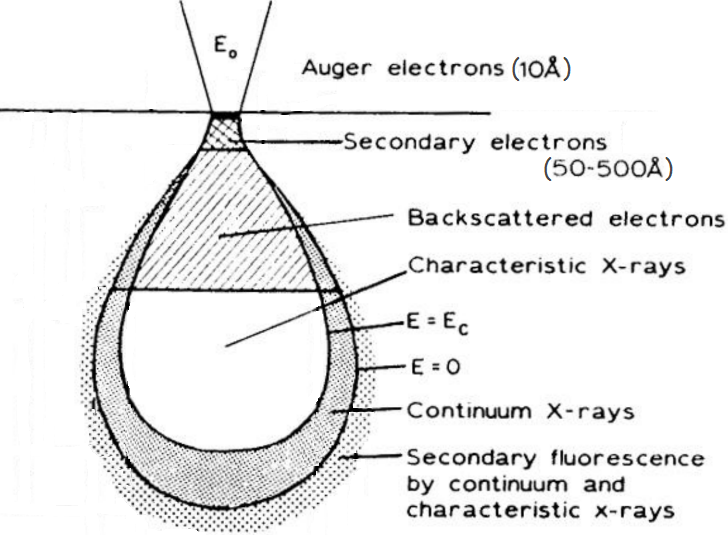
\includegraphics[width=0.6\linewidth]{sem_interaction_volume.png}
    \caption[Range and spatial resolutions of backscattered electrons, secondary electron, X-rays, and Auger electrons produced from a SEM.]{Range and spatial resolutions of backscattered electrons, secondary electron, X-rays, and Auger electrons produced from a scanning electron microscope. The outline of the volume of characteristic X-ray production is defined by the case where the electron energy $E$ is just sufficient to produce X-rays requiring the critical energy $E_c$, which varies with the X-ray of interest. The outline of the volume of continuum X-ray (bremsstrahlung) production is where $E$ is zero and cannot be decelerated any longer \citep[Reprinted from][]{goldstein2012scanning}.}
    \label{fig:sem_interaction_volume}
\end{figure}

Absolute concentration values of the elements are obtained using P/B-ZAF analysis. The peak-to-local-bremsstrahlung-background ratios (P/B) are input to a modified ZAF matrix correction, which relates the recorded spectrum to the primary rate of X-ray generation. This is done mainly based on analytical expressions to correct for atomic number depended X-ray yield (Z), self-absorption (A), and secondary fluorescence enhancement (F) \citep{quantax2008microanalysis}. Since P/B-ZAF do not use explicit or implicit standards in the calculation of concentrations, it is called a true standardless method.%, and self-calibrating.

 %using the P/B-ZAF algorithm the characteristic X-ray intensities (i.e. the net peak areas) are calculated in relation to the mean level of the simultaneously recorded bremsstrahlung background

%%=========================================
\section{X-ray Photoelectron Spectroscopy}\label{sec:xps}
\Acf{xps} is used to find the elemental composition of the outer surface of a solid (\SI{\sim 100}{\angstrom}). In addition, \ac{xps} can be used to get information about the chemical binding state of the detected elements.

\Ac{xps} is based on the emission and detection of photoelectrons. The sample is bombarded with a beam of X-ray photons of energy $E_\text{photon}$. If $E_\text{photon}$ is sufficiently large, i.e. greater than the binding energy of an electron $E_\text{binding}$, it can kick out the electron from an inner shell in an atom. If the photoelectron is close to the surface, it can be emitted from the sample to the vacuum outside, with a kinetic energy given by
\begin{equation}
    E_\text{kinetic} = E_\text{photon} - E_\text{binding} - \phi,
\end{equation}
where $\phi$ is the work function that accounts for the loss of energy as the electron leaves the sample and is absorbed by the detector. The detector measures the kinetic energy of the emitted photoelectron. Since the electron binding energies are at discrete energy levels, and these are element and chemical-bonding state dependent, a spectrum of the number of emitted electrons as a function of binding energy reveals which elements are present in the sample and their chemical-bonding state.

The mean free path of the photoelectrons in a material is on the order of \SI{20}{\angstrom} \citep{tanuma1991calculations}. Hence, only electrons emitted from atoms within a few mean free paths from the surface, i.e. \SI{80}{\angstrom}, are able to escape the material without loss of energy and be detected as peaks in the spectra. This makes \ac{xps} a surface sensitive technique that can tell us about the outermost layer of the sample. The electrons that are scattered inelastically before leaving the sample form the continuous background of the spectrum.

Quantification of the composition in the sample can be made by finding the ratios of the peak areas for the elements found in the sample. The atomic fraction of element $A$ in a homogeneous solid is estimated to be \citep{moulder2000handbook}
\begin{equation}\label{eq:xps_concentration}
    C_\mathrm{A} = \frac{I_\mathrm{A}/S_\mathrm{A}}{\sum_i I_i/S_i},
\end{equation}
where $I_\mathrm{A}$ is the measured peak area for element A, and analogously for $I_i$; and $S_\mathrm{A}$ is the sensitivity factor of element A, and analogously for $S_i$. The sensitivity factors take into account parameters that affect the intensity of the element, such as the distinctive cross-sections and densities of the different elements, and normalise these to that of the most intense peak. %the beam experience as it collide with the elements in the sample, that increase or decrease the probabilities for exciting a photoelectron.
% where $I_\mathrm{A}/I_i$ is the measured peak area for element A/$i$ and $S_\mathrm{A}/S_i$ is the sensitivity factor of element A/$i$.

A simple model for an abrupt uniform layer L on a bulk material B is used to estimate the thickness $d$ of a layer. The ratio between the signal from the layer and the signal from the bulk as a function of $d$ is given by \citep{briggs1990practical} 
\begin{equation}\label{eq:signal_ratio}
    R(d) = \parentheses{\frac{a_\mathrm{B}}{a_\mathrm{L}}}^3 \frac{\lambda_\mathrm{LL}}{\lambda_\mathrm{BB}} \frac{1-\exp{\parentheses{-\frac{d}{\lambda_\mathrm{LL}\cos\theta}}}}{\exp{\parentheses{-\frac{d}{\lambda_\mathrm{BL}\cos\theta}}}},
\end{equation}
where $a_\mathrm{B}$ is the atomic size of material B, and analogously for $a_\mathrm{L}$; and $\lambda_\mathrm{BL}$ is the inelastic mean free paths of photoelectrons emitted from material B in layer L, and analogously for $\lambda_\mathrm{BB}$ and $\lambda_\mathrm{LL}$. The atomic size is derived from $1000\rho_\mathrm{M}N a_\mathrm{M}^3 = A_\mathrm{M}$, where $\rho_\mathrm{M}$ is the density, $N$ is Avogadro's number, and $A_\mathrm{M}$ is the mean atomic weight of the matrix atoms. The inelastic mean free path is predicted by the model of \citet{tanuma1991calculations}.
% where $a_\mathrm{B}$ and $a_\mathrm{L}$ are the atomic size of material B and L respectively, $\lambda_\mathrm{BB}$ and $\lambda_\mathrm{BL}$ are the inelastic mean free path of photoelectrons emitted from B in B and L respectively, and $\lambda_\mathrm{LL}$ are the inelastic mean free path of photoelectrons emitted from L in L. 
%\mycomment{Do I need to include more equations?}.
%Atomic size is given by
%\begin{equation}
%    a = \parentheses{\frac{m }{\rho N_\mathrm{A}}}^{1/3},
%\end{equation}

%All elements from \ce{^3Li} to \ce{^92U} are detectable if they exist at $>0.05 \text{ atomic} \%$ \citep{vanderHeide2011X-ray}.
%of less than \SI{10}{\nano\metre} of the outer solid surface.

%XPS
%E_k = h\nu - E_B - \phi_s 1-10\mu m penetrating depth but the free path of electrons are only tens of angstroms surface sensitive the information about the sample surface is obtained by analyzing the energies of the emitted electrons qualitative analysis (put line positions for the elements relevant to this work in an appendix)
%n1(n2 = I1/S1 / (I2/S2)
%Cx = nx / sum_i ni
%gives semi-qualitative results within 10-20\%(Moulder et al. 1995)

%AFM
%TEM
%RHEED

%%=========================================
\section{Atomic Force Microscopy}\label{sec:afm}
\Acf{afm} is used to obtain high-resolution topographic images of a sample surface. While \ac{sem} provides two-dimensional images without information about depth or height of the defects, \ac{afm} can provide three-dimensional topographical images of the defects with the highest vertical resolution among all techniques \citep{smith2013industrial}. The \ac{afm} is a type of \ac{spm} that measures the surface topography by raster scanning a cantilever with a sharp tip over the sample surface. As the tip approaches the sample surface, forces between the tip and the surface lead to a deflection of the cantilever according to Hooke's law \citep{bhushan1998handbook}
\begin{equation}
F = -k\Delta x
\end{equation}
where the force $F$ is directly proportional to the cantilever spring constant $k$ and the cantilever deflection $\Delta x$. The forces due to electrostatic repulsion dominate when the tip is close to the surface and cause the cantilever to deflect away from the surface, while the attractive van der Waals forces between the surface and the tip dominate when the tip is further away and cause the cantilever to deflect towards the surface.

Cantilever deflections towards or away from the surface are monitored with laser light from a solid-state diode that is focused on the back of the cantilever and reflected onto a \ac{pspd}, as seen in Fig.~\ref{fig:afm_laser}. As the tip scans the sample, the raised and lowered features on the sample surface cause the cantilever to deflect, which in turn change the direction of the reflected laser beam that is detected by the \ac{pspd}. The resulting image is a topographic map of the sample surface features. The lateral resolution of the images is around \SI{30}{\nano\metre} while the vertical resolution can be up to \SI{0.1}{\nano\metre} \citep{birdi2003scanning}.

%The image of the surface is obtained by scanning with a very sharp tip. When the tip is further away then van der Waals attractive forces dominate between the tip and the surface. However, if the tip is close enough to the surface, electrostatic repulsive forces dominate.

%The tip is attached to a cantilever and if the tip interacts with a surface feature then the cantilever bends. The force needed to bend the cantilever is described by Hook's law, $F=-k\Delta x$ where the force directly depends on the cantilever spring constant $k$ and the cantilever deflection $\Delta x$.

%The cantilever deflection is monitored with a laser beam which is focused on the cantilver and the light is reflected on a detector. If the cantilever bends the position of then the laser beam changes.

There are three basic \ac{afm} imaging modes: contact mode, non-contact mode, and tapping mode. Contact mode is, as the name implies, a technique where the tip is in contact with the surface during the scan. In the case of non-contact mode the tip is vibrating, with a constant frequency near the resonant frequency of the tip, above the surface. In tapping mode the tip is closer to the surface and vibrates with a higher amplitude than in non-contact mode. In the lowest point of the trajectory, the tip is briefly touching the surface.

\begin{figure}[htbp]
    \centering
    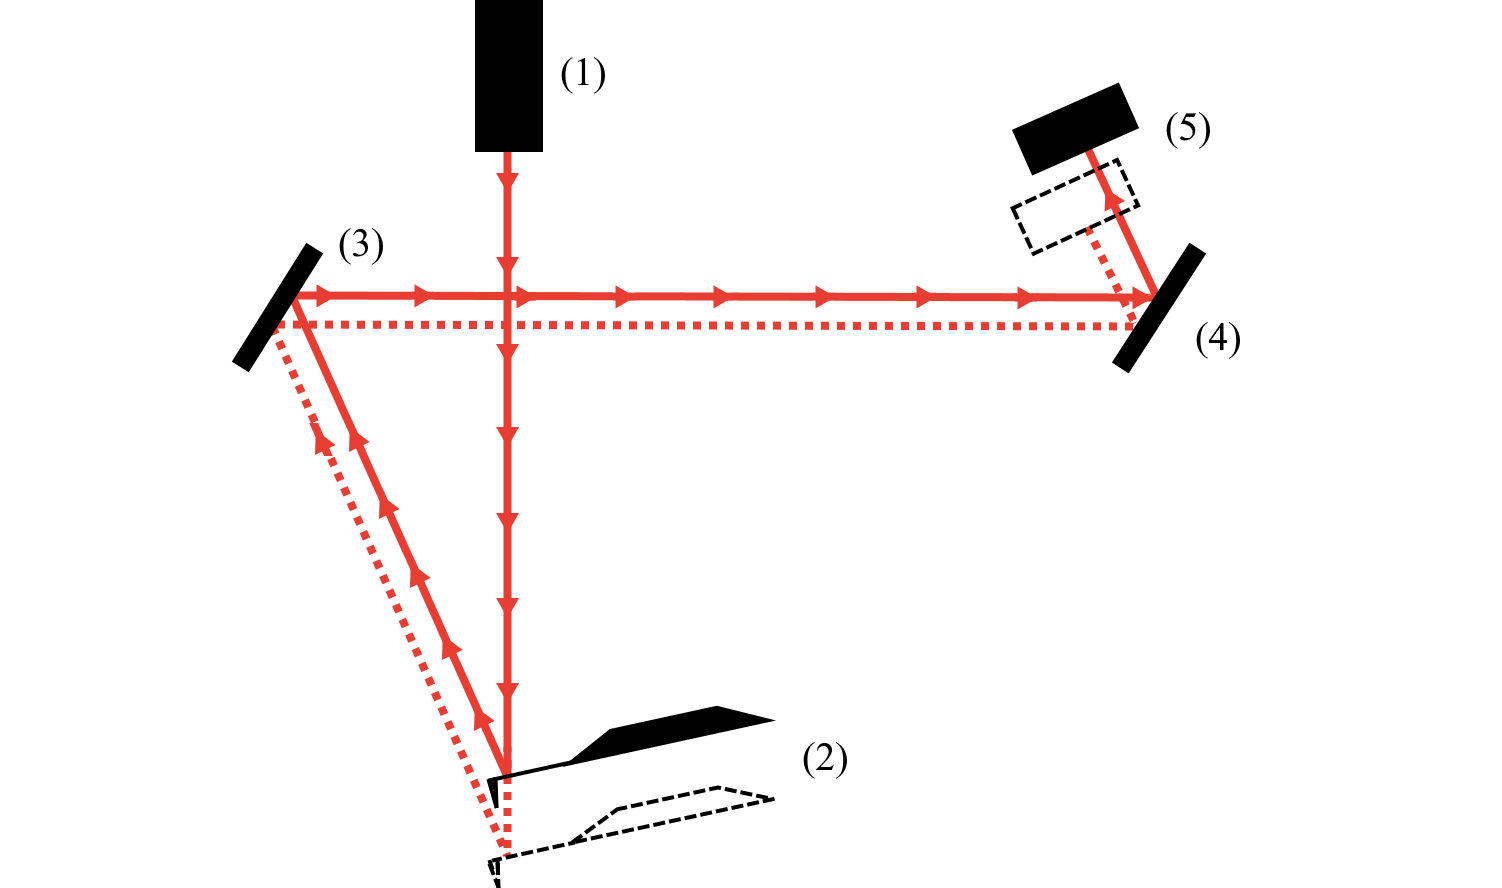
\includegraphics[width=1.0\linewidth]{afm_principles.png}
    \caption[Illustration of the principles behind \ac{afm}.]{Illustration of the principles behind \ac{afm}. The setup consists of: (1) laser, (2) cantilever with a sharp tip, (3) steering mirror, (4) stationary mirror, and (5) \acf{pspd}. The red line represents the laser beam and the dotted red line show how the path is changed by the deflection of the cantilever \citep[Adapted from][]{psia2002xe100}.}
    \label{fig:afm_laser}
\end{figure}

An \ac{afm} image is a convolution between the tip and the sample which is to be visualised. Therefore, the tip radius limits the lateral resolution, and cause an image artefact which is observable when using a tip with a similar or higher radius of curvature with respect to the feature. Holes can appear both narrower and less deep, and protruding features can appear wider than they really are, see Fig.~\ref{fig:afm_tip-convolution}. For the technique to provide information of the surface at the atomic level, the tip must be sharp, ideally terminating in just a single atom on the tip. Any changes to the tip that cause it to become broader, will decrease the lateral resolution of the image. These changes might be caused by contaminants on the tip or wearing of the tip due to collisions with the sample by either scanning too fast or having a rough surface \citep{birdi2003scanning}.

\begin{figure}[htbp]
    \centering
    \mySubfigure{0.49\linewidth}{afm_artifact_small-tip.png}[fig:afm_artifact_small]
    \hfill
    \mySubfigure{0.49\linewidth}{afm_artifact_big-tip.png}[fig:afm_artifact_large]
    \caption[Illustration of the convolution effect in an \ac{afm} image due to tip size.]{Illustration of an \ac{afm} image artefact that is caused by the convolution effect between the tip and the feature which is to be visualised, i.e. a broadening effect. This image artefact is observable when using a tip with \subref{fig:afm_artifact_small} a similar or \subref{fig:afm_artifact_large} higher radius of curvature with respect to the feature being imaged. In the images, grey represents the probe tip, black represents the real surface and surface features, and red represents the displayed surface \citep[Adapted from][]{psia2002xe100}.}
    \label{fig:afm_tip-convolution}
\end{figure}

\subsection{Surface Roughness}

Surface roughness is used as a quantitative measurement of surface changes. Surface roughness refers to height variations on the surface in the direction of the normal vector of a reference plane. There are many ways to characterise roughness, but one of the most commonly used for describing \ac{afm} images is the \ac{rms} roughness \citep{eaton2010atomic}. \Ac{rms} roughness is a statistical parameter given by \citep{thomas1999amplitude}
\begin{equation}\label{eq:rmsroughness}
R_\textrm{q} = \sqrt{\frac{1}{N}\sum_{i=1}^{N}\brackets{z_i-\bar{z}}^2},
\end{equation}
where $N$ is the number of data points in the image, $z_i$ is the height at point $i$, and $\bar{z}$ is the average elevation of the image profile. %reflects the roughness of the sample and is obtained by the Fourier Transform of the image.

%%=========================================
\section{Fourier Transform Infrared Spectroscopy}\label{sec:ftir}
\Acf{ftir} is a technique that is used to obtain an \ac{ir} transmission spectrum of a material. The spectrum indicates how much light that is transmitted through the sample at each wavelength. Patterns in the spectrum can help identify impurities and contaminants in the sample since molecules exhibit specific \ac{ir} transmission fingerprints \citep{smith2011fourier}.

The transmittance spectrum, the percentage of incoming light that is transmitted through the sample as a function of wavenumber, is found by calculating the ratio of the sample spectrum and the background spectrum. The background spectrum is usually acquired immediately before the sample is placed in the sample compartment to get as identical conditions as possible.

\begin{figure}[htbp]
    \centering
    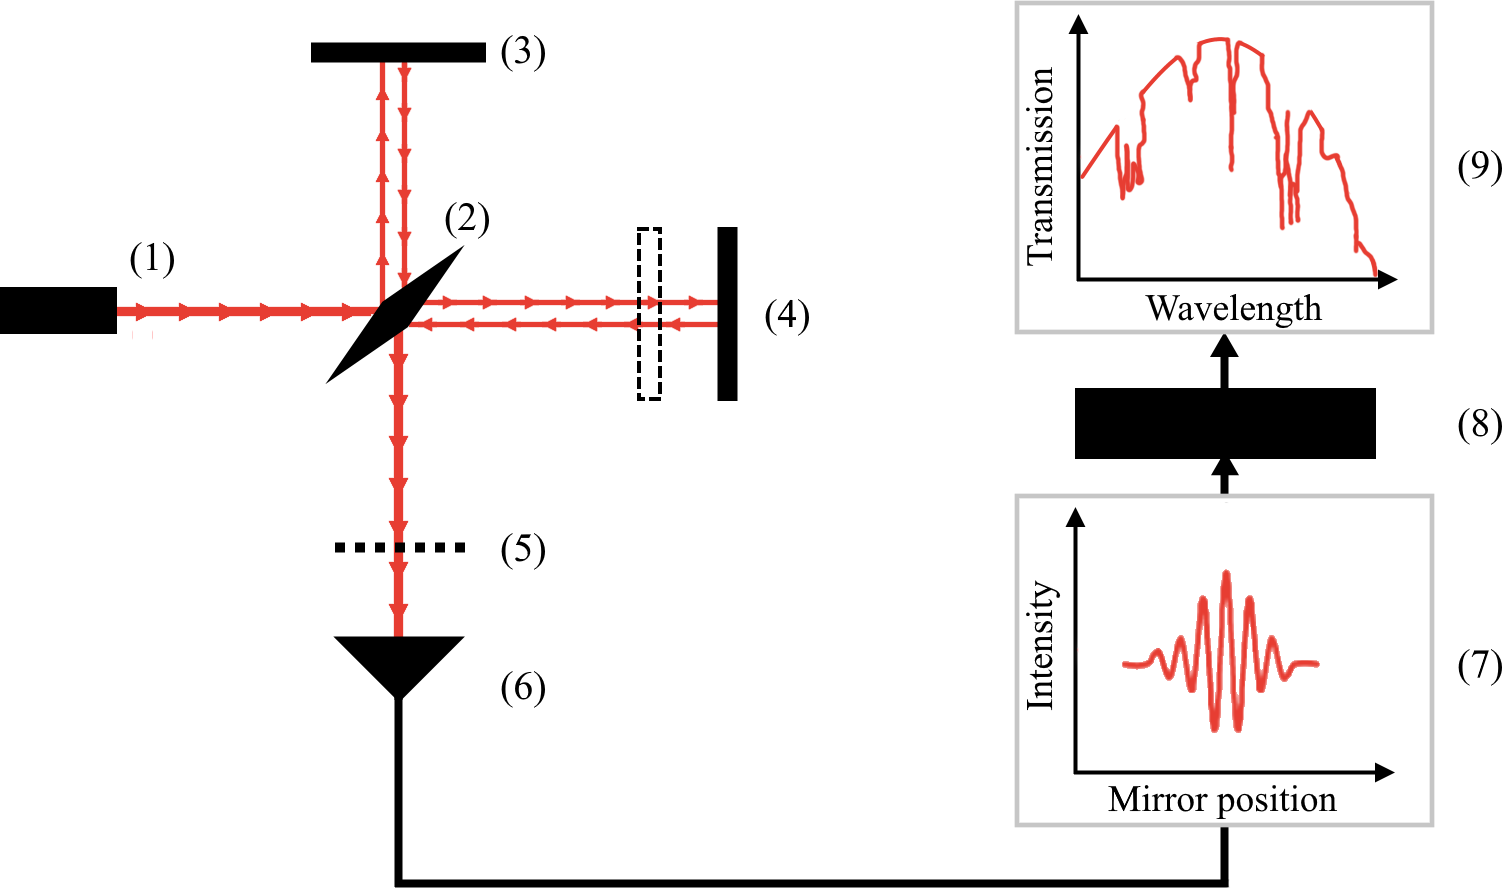
\includegraphics[width=1.0\linewidth]{ftir_principles.png}
    \caption[Illustration of the principles behind \ac{ftir}.]{Illustration of the principles behind \ac{ftir}. The setup consists of: (1) light source, (2) beamsplitter, (3) fixed mirror, (4) movable mirror, (5) sample compartment, (6) detector, (7) interferogram, (8) Fourier transform, and (9) \ac{ir} transmission spectrum \citep[Adapted from][]{nicolet2001introduction}.}% A beam of photons is first shone into a Michelson interferometer where the beamsplitter splits the light into two beams. One beam is refracted towards the fixed mirror and the other is transmitted towards the movable mirror. The beams are reflected back and combined at the beamsplitter. The resulting interference pattern is directed to the sample, and the detector measures how much of the beam that is transmitted through the sample as a function of mirror position, known as an interferogram. A Fourier transform is used to find how much each wavelength contributes to the signal, and convert the interferogram to a spectrum that show the intensity of the beam that is transmitted as a function of wavelength.}
    \label{fig:ftir_michelson}
\end{figure}

A beam of photons -- containing a range of wavelengths -- is first shone into a Michelson interferometer before it hits the sample. The Michelson interferometer contains a beamsplitter, which splits the light source into two. One beam is refracted towards a fixed mirror and the other is transmitted towards a movable mirror. The beams are reflected back towards the beamsplitter where they recombine, see Fig.~\ref{fig:ftir_michelson}. The difference in optical path length between the two beam paths, known as the \ac{opd}, is adjusted by moving the movable mirror. The resulting interference pattern is directed to the sample, and the detector measures how much of the beam that is transmitted through the sample as a function of mirror position, known as an interferogram.

As the mirror moves continuously from an \ac{opd} of zero to a distance further away, the intensity pattern of one specific wavelength $\lambda$ goes from constructive interference at \ac{opd}$=0$ to destructive interference where \ac{opd}$=(n+\frac{1}{2}) \lambda$ and constructive interference where \ac{opd}$= n \lambda$ for $n\in\mathbb{N}$. Waves which are not completely in or out of phase will have an intermediate intensity pattern. The interferogram is the sum of the interference patterns from all the different wavelengths measured at many discrete mirror positions. A Fourier transform is used to find how much each wavelength contributes to the signal, and converts the interferogram to a spectrum that shows the intensity of the beam that is transmitted as a function of wavelength \citep{smith2011fourier}.

%Since the Michelson interferometer has only a finite maximum \ac{opd}, it do not meet the requirements of the Fourier transform that the interferogram should be integrated from $-\infty$ to $+\infty$ \citep{bretzlaff1986apodization}.
%A problem that is encountered while doing 
%
%The resolution of the spectrum is set by the range of the mirror
%
The band gap of a material can be determined from the \ac{ftir} spectrum as the wavelength where the transmission increases steeply with increasing wavelength. The increase in transmission occurs because the photons with energy greater than the band gap can be absorbed by the creation of an electron-hole pair, while photons with energy less than the band gap cannot and are transmitted.

The thickness of a thin layer on top of another material can be calculated from the \ac{ftir} spectrum. Both the surface of the layer and the boundary between the layer and the underlying material reflect the incoming beam of photons. This difference in optical path length causes constructive and destructive interference of the light, which manifests as a fringing effect in the \ac{ftir} spectrum. The maxima are found where the optical path difference equals an even number of wavelengths. Hence, the fringes in the spectrum can be used to determine the thickness of the film
\begin{equation}
\label{eq:ftir_thickness}
d = \frac{1}{2}\frac{1}{n\Delta k},
\end{equation}
where $n$ is the refractive index and $\Delta k$ is the average period for one fringe \citep{griffiths2007fourier, stuart2008modern}.
%
%%=========================================

%%%=========================================
%\chapter{About \ce{CdZnTe}}
%%=========================================
%\ce{CdZnTe} is a compound semiconductor material composed of elements belonging to the II and VI groups of the periodic table of chemical elements.

%\section{Crystal structure}
%The crystal structure of \acl{czt} consist of two face centred cubic lattices with one shifted from the other by $\frac{1}{4}$ of the distance along the (111) direction. One lattice is occupied by \ce{Te} and a fraction $x$ of the other lattice is occupied by \ce{Zn} while the remaining fraction of the other lattice is occupied by \ce{Cd}.
%%=========================================
%\section{Band structure}
%Figure~\ref{fig:} clearly demonstrates that the band gap of \ac{mct} can be tuned to .. \mycomment{???}
%%=========================================
\chapter{Experimental Details}\label{ch:exp-details}
In this chapter, a description of the substrates, the pre-growth surface preparation methods, and the experimental equipment is presented.

\section{Epitaxy}

Epitaxy refers to the growth of a crystalline layer with a well-defined orientation determined by the crystal structure of a substrate. One of the epitaxial growth techniques is \acf{lpe} where a layer is grown from a supersaturated liquid solution on a substrate. The process starts with heating the solution, followed by a period where impurities are baked out. After this the temperature is lowered to equilibrium, and then the the growth is achieved by reducing the temperature so that the material deposit on the substrate. Another epitaxial growth technique is \acf{mbe} where a source material is heated to produce an evaporated beam of particles. Then the constituent elements of the wanted material are transported through vacuum from the sources to the substrate where it condense.

%%=========================================
\section[\ce{Cd_{1-y}Zn_yTe} Substrates]{\ce{Cd_{1-y}Zn_yTe} Substrates% TOC, section title, header, header
       \sectionmark{CZT Substrates}}\sectionmark{CZT Substrates}
%\todo{CZT advantages: excellent lattice match, CT good passivation. Disadvantage: brittle brakes easily, expensive.}

\Acl{czt} substrates with $y=\SI{0.04}{}$ are mainly \ce{CdTe} with a small fraction of the \ce{Cd} atoms replaced by \ce{Zn} atoms in order to match the substrate lattice constant to that of \acl{mct} (\SI{6.46}{}-\SI{6.48}{\angstrom}). \Ac{czt} has a zincblende structure with two interpenetrating face-centered cubic lattices offset by $\parentheses{\frac{1}{4},\frac{1}{4},\frac{1}{4}}a$, where $a$ is the lattice constant in the primitive cell. Cadmium or zinc atoms form one of the sublattices while tellurium atoms form the other, as seen in Fig.~\ref{fig:zincblende-structure}.

\begin{figure}[htbp]
    \centering
    \mySubfigure{0.302\linewidth}{zinc-blende.png}[fig:zincblende-structure]
    \hfill
    \mySubfigure{0.679\linewidth}{zinc-blende_faces.png}[fig:zincblende-face]
    \caption[Crystal structure of \ac{czt}.]{Illustration of \subref{fig:zincblende-structure} the zincblende crystal structure of \ac{czt} and \subref{fig:zincblende-face} the difference between the two faces of a (111)-oriented \ac{czt} substrate (or the (111)-oriented steps in a (211)-oriented substrate). The plane will have top and bottom surfaces that are slightly different: the A face is terminated by triply bonded \ce{Cd} (or \ce{Zn}) or singly bonded \ce{Te}, while the B face is terminated by triply bonded \ce{Te} or singly bonded \ce{Cd} (or \ce{Zn}). \ce{Cd} (or \ce{Zn}) atoms form the white sublattice and \ce{Te} atoms form the black sublattice \citep[Adapted from][]{sivananthan1986relation}.}
    \label{fig:zincblende}
\end{figure}

The orientation of the substrate is given by the surface crystallographic plane, and for \ac{czt} substrates the crystal is cut to give surface plane (111) for \ac{lpe} growth and (211) for \ac{mbe} growth. The (211)-oriented substrate consists of steps that are (111)-oriented. A substrate cut along these planes will have top and bottom surfaces that are slightly different: one surface will be terminated by triply bonded \ce{Cd} (or \ce{Zn}) or singly bonded \ce{Te}, and is called the \emph{A} face, while the other side of the substrate will be terminated by triply bonded \ce{Te} or singly bonded \ce{Cd} (or \ce{Zn}), and is called the \emph{B} face \citep{sivananthan1986relation}, see Fig.~\ref{fig:zincblende-face}. \Ac{mct} films are always grown on the B face of the substrate since it is less sensitive to misorientation \citep{parker1988terracing, edwall1984liquid}.%$y$ is the fraction of cadmium that is substituted with zinc and $1-y$ is the fraction of cadmium \citep{zha2005atomic}. \Ac{czt}

In this study, two (111)B-oriented substrates from different manufacturers and one (211)B-oriented substrate have been studied. Substrate A is a $\SI{30}{\milli\metre}\times\SI{30}{\milli\metre}$ state-of-the-art (111)B-oriented \ac{czt} substrate from the Japanese firm JX Nippon Mining \& Metals Corporation (vendor A). The fraction of \ce{ZnTe} in substrate A is \SIrange{2.8}{3.6}{\percent}. Substrate A was compared to substrate B -- a $\SI{30}{\milli\metre}\times\SI{30}{\milli\metre}$ (111)B-oriented \ac{czt} substrate -- from an alternative source (vendor B). Substrate B has \SI{\sim 4}{\percent} \ce{ZnTe} and \SI{\sim96}{\percent} \ce{CdTe}. Substrate C is a $15\times$\SI{15}{\milli\metre^2} state-of-the-art (211)B-oriented \ac{czt} substrate also from vendor A. The fraction of \ce{ZnTe} in substrate C is \SIrange{2.6}{3.4}{\percent}. % vendor B: Klamnik, Keystone

Images of the substrates can be seen in Fig.~\ref{fig:substrateABC}. Relative terms, such as \emph{upper}, \emph{lower}, \emph{left}, \emph{right}, and \emph{centre}, are used to describe the locations on the substrate surfaces throughout the thesis. These relative terms are related to the orientation depicted in Fig.~\ref{fig:substrateABC}. When coordinates are given, they are measured from the lower left corner of the substrate surfaces. %\todo{Nevne koordinatsystem her? Eller droppe koordinater og heller bruke lower left corner, etc.?}

The substrates were characterised as-received and after surface pre-growth preparation. The latter was either polishing and etching or just etching if the substrate was already polished by the vendor. Then \iac{mct} layer was grown on each substrate and characterised with emphasis on correlation between defects in the \ac{mct} layer and particles, impurities, defects and roughness of the substrates.

Unfortunately, after being characterised both as-received and after polish and etch, substrate B broke in two pieces when mounting for the final \ac{ftir} mapping before \ac{mct} growth. One piece shattered further when it fell on the floor, as seen in Fig.~\ref{fig:subBb_photo_pieces}. These substrates are brittle, and all the handling of the substrate through two rounds of characterisation with various techniques had made it even more so. A new $\SI{30}{\milli\metre}\times\SI{30}{\milli\metre}$ (111)B-oriented \ac{czt} substrate from vendor B, substrate B2, was polished and characterised before growing \iac{mct} layer on it.
%Substrate B was unfortunately shattered during preparation for \ac{ftir} even though the preparation procedure was followed as normal, see Fig.~\ref{fig:subB_om_6x_pieces}. It could be the additional handling, i.e. due to the extensive characterisation, that caused it to be more fragile. Substrate B was already studied as-received and with surface pre-growth preparation (except for \ac{ftir}). The next step was to grow \iac{mct} film on it. To be able to fulfil the process, an additional substrate from vendor B was studied (substrate B2). Substrate B2 is a $\SI{30}{\milli\metre}\times\SI{30}{\milli\metre}$  (111)B-oriented \ac{czt} substrate and has \SI{\sim 4}{\percent} \ce{ZnTe} and \SI{\sim96}{\percent} \ce{CdTe}. Due to lack of time, substrate B2 was only studied after surface pre-growth preparation before \iac{mct} film was grown on it.

\begin{figure}[htbp]
    \centering
    \mySubfigure{0.49\linewidth}{subAa_om_6x.png}[fig:subAa_photo]
    \hfill
    \mySubfigure{0.49\linewidth}{subBb_om_6x.png}[fig:subBb_photo]
    \par\bigskip
    \mySubfigure{0.49\linewidth}{subB2b_om_6x.png}[fig:subB2b_photo]
    \hfill
    \mySubfigure{0.49\linewidth}{subCa_om_6x.png}[fig:subCa_photo]
    \par\bigskip
    \mySubfigure{0.49\linewidth}{subBb_om_pieces.png}[fig:subBb_photo_pieces]
    \caption[Optical microscopy images of the substrates.]{Optical microscopy images of the substrates. \subref{fig:subAa_photo} Substrate A -- as-received, $\SI{30}{\milli\metre}\times\SI{30}{\milli\metre}$, (111)B-oriented from vendor A; \subref{fig:subBb_photo} substrate B -- after polish and etch, $\SI{30}{\milli\metre}\times\SI{30}{\milli\metre}$, (111)B-oriented from vendor B; \subref{fig:subB2b_photo} substrate B2 -- after polish and etch, $\SI{30}{\milli\metre}\times\SI{30}{\milli\metre}$, (111)B-oriented from vendor B; \subref{fig:subCa_photo} Substrate C -- as-received, $\SI{15}{\milli\metre}\times\SI{15}{\milli\metre}$, (211)B-oriented from vendor A; and \subref{fig:subBb_photo_pieces} substrate B after it shattered during mounting for \ac{ftir}.}
    % \todo{Optical microscopy images of the substrates. a) Substrate A: Asreceived, 30x30mm2 from vendor A, b) .. and 15x15mm2 substrates}
    \label{fig:substrateABC}
\end{figure}

Vendor A sells both (111)B-oriented substrates for \ac{lpe} growth and (211)B-oriented substrates for \ac{mbe} growth. The (211)B substrates are cut at an angle of \SI{19}{\degree} with the (111) planes. This gives a surface with (111)-oriented atomic steps, and the resulting step-flow growth improves the crystallinity of the \ac{mbe} film because atoms land on the surface and diffuse to a step edge before they nucleate, and hence, reduce the change of dislocations. 

High quality substrate surfaces are crucial for growth of high quality films. After cutting, the substrates must be polished to obtain the necessary smooth and planar surface. Finally, an etch is needed to remove polishing products that have been trapped in the substrate during polishing. In \ac{lpe} growth, the outermost layers of the substrate are initially melting in the liquid growth material before the temperature falls and the film starts to grow on the surface. Therefore, some surface defects can be less important while others remain and affect the grown film.

%Substrates from two vendors were compared: One state-of-the-art \ac{lpe} substrate (substrate A) and one state-of-the-art \ac{mbe} substrate (substrate C) from the Japanese manufacturer JX Nippon Mining \& Metals Corporation (vendor A), and one \ac{lpe} substrate (substrate B) from an alternative source (vendor B). Substrate A and B was polished by the vendor and needed only a short etch before growth, while substrate B required both polishing and etching before growth.
%
%% The substrates:
% --- A:  with lot number BZ1503 and wafer number ID7.1, Zn concentration Specification 0.025+-0.05 Measurements 0.028-0.036
% --- B:  with number C-3895-23
% --- B*: with number C-4040-8
% --- C:  with lot number BZ1204 and wafer number ID10.4, Zn concentration Specification 0.035+-0.01 Measurements 0.026-0.034

%%=========================================
\section{As-Received}
The substrates were removed from the box they came in and directly mounted on carbon tape on a \ac{sem} holder before \ac{sem} was performed. To ensure that the removal process would be as easy as possible, the carbon tape was made almost non-sticky by touching the tape multiple times with a cleanroom glove. A magnetic plate was attached underneath the \ac{sem} holder with double-sided tape when \ac{afm} was performed. 

To remove the substrate from the \ac{sem} holder, the holder with the substrate on top was placed in a beaker and acetone was poured into the beaker up to right below the backside of the substrate. The acetone dissolved the carbon tape so that it was possible to get a scalpel under the substrate and push the substrate off. %\todo{Mention problems with tape removal.}

%%=========================================
\section{Pre-Growth Surface Preparation}
Substrate preparation is an important part before the deposition of a crystalline layer takes place because it is important to have the surface as smooth and flat as possible and without any particles. The three substrates were prepared in the following way: Substrate A and C needed only an etch before growth, as described below, since they were already sufficiently polished by the vendor. Substrate B and B2 needed a final polish as part of their pre-growth preparation in addition to an etch, as described below, since they only had been through a coarse polish by the vendor.

\subsection{Etching of Substrate A}\label{sec:subA_etch}

After the characterisation of the as-received substrate A was completed, the substrate went through a standard \ac{lpe} \ce{Br}:methanol preparation etch procedure. First, the substrate was cleaned using a two-solvent method. The two-solvent cleaning procedure consists of placing the substrate for \SIrange{2}{3}{\minute} in each of four containers: two with boiling acetone, one with boiling methanol, and one with methanol at room temperature. Before further preparation, the substrate is blown dry with gaseous nitrogen. Then, the the substrate was etched in an etch consisting of \SI{0.25}{\milli\litre} bromine and \SI{40}{\milli\litre} methanol for \SI{30}{\second} while stirring every \SIrange{1}{2}{\second}. Finally, the substrate was rinsed with methanol to remove any etch residues. This \ce{Br}:methanol etch procedure was repeated before \ac{lpe} growth with an etch time of \SI{50}{\second} to remove possible contaminants from the characterisation of the etched substrate. %When the substrate is lifted from one container, it is rinsed with \todo{skriv ned det steget her.}

\subsection{Polishing and Etching of Substrate B}

After the characterisation of the as-received substrate B was completed, the substrate was cleaned using soap, rinsed with purified water, and then blown dry with gaseous nitrogen. This is the standard \ac{lpe} preparation procedure before polishing and etching takes place, but due to the exposure during characterisation and the potential residue of carbon tape underneath the substrate, it had to go through an additional cleaning procedure with a two-solvent method, as explained in Section~\ref{sec:subA_etch}.%\todo{mention that this was not enough, maybe?}

%The as-received substrate A was etched \todo{with a Bromine-based etch}. The substrate was already polished when received from the vendor.
%
% Sprutet på såpe over hele substratet. Skylt av med renvann. Blåst tørr med nitrogen. 
% Vanligvis kun såpe, men nå kokende aceton og metanol pga. det kan sitte igjen litt karbonteip fra holderen. Lagt i kokende aceton i noen få minutter, skylt med aceton fra spruteflaske for å få vekk det som har løsnet og ikke få det med videre, lagt i kokende aceton igjen noen få minutter, sprutet med aceton deretter metanol før lagt i kokende metanol noen få minutter, spylt med metanol, og til sist lagt i romtemperert metanol i noen minutter. Blåst tørr med nitrogengass.
% Montert på glassplate med Crytalbond. Varmer opp Crystalbond slik at det smelter og renner under substratet. Avkjøles. Sitter fast.
% Festet opp ned i jig med vakuum på glassplata. Roterende skive med hard poleringspad pusser substratet plant, 50 um. Bytter til myk poleringspad og pusser substratet jevnt, 30 um, 111 minutter. Drypper på poleringsvæske jevnt og trutt (med pumpe). Kjell Ove har også på "lubricat" når skiva begynner å gå litt sakte (alkohol og ++).
% Skyller med renvann. Blåser tørr med nitrogen.
% Fjernet poleringssøl som har samlet seg langs med endekantene ved bruk av q-tips. Drar de langs med kanten. Bruker en bred q-tip til å fjerne det som ligger på glassplaten. Det legger seg mye poleringssøl langs endekantene. Sannsynligvis oppå substratet også.
% Spruter på såpe over hele substratet. Har såpe på en bomullsdott og drar denne over substratet forsiktig. Tar ny bomullsdott og bløter og drar over.
% Skyller med aceton. Blåser tørr med nitrogen.
% Varmer opp glassplata på varmeplate (150 grader celsius) slik at Crystalbond smelter, og det er mulig å skyve av substratet med hjelp av en spatel. Og over i en hvit rund silplate med stang til å duppe opp og ned i begerglass.
% Samme kokende aceton og kokende metanol prosedyre som over.
% Ligger i romtemperert metanol over natta (fra 20.03.17 14.00 til 21.03.17 12.00).

The as-received substrate B was polished with alumina powders with abrasive size of \SI{50}{\nano\metre} using a Struers LaboPol-5 polishing jig. First the substrate was planarised by removing an average of \SI{80}{\micro\metre} of material from the surface of the substrate with a hard polishing pad for \SI{200}{\minute}. Then a smoother finish was achieved by removing another \SI{30}{\micro\metre} of material from the surface using a soft polishing pad for \SI{111}{\minute}. The soft polishing pad conforms to local topology variations on the nanoscopic scale, and thus, makes the surface smooth, while hard pads do not \citep{lee2000nanotopography}. The polishing slurry consists of \SI{50}{\nano\metre} colloidal alumina particles and soap dissolved in methanol. The use of soap as a lubricant is helpful in prolonging the life of the polishing jig.

During polishing the substrate was attached to a plate using Crystalbond mounting compound. The Crystalbond was melted underneath the substrate to form an adhesive bond between the substrate and the mounting plate when solidifying. After the polishing process was completed, the mounting plate was heated to melt the Crystalbond so that the substrate could be pushed off. Then the remaining Crystalbond was dissolved and removed through the same two-solvent cleaning procedure as before polishing. The cleaned substrate was soaked in a beaker with methanol at room temperature over night before it was etched with a \ce{Br}:methanol etch the following day, as described for substrate A in Section~\ref{sec:subA_etch}, and quickly inserted into the \ac{sem}.

\subsection{Etching of Substrate C}
%The as-received substrate C was etched \todo{with a Bromine-based etch}. The substrate was already polished when received from the vendor.

After the characterisation of the as-received substrate C was completed, the substrate went through a standard \ac{mbe} \ce{Br}:methanol preparation etch procedure: First, the substrate was cleaned with methanol and acetone: A thin layer of methanol was left on the surface for \SIrange{2}{3}{\second} before it was blown dry with gaseous nitrogen, and the equivalent was repeated with acetone and finally with methanol for the second time. Then, the substrate was etched in \SI{1}{\percent} \ce{Br}:methanol for \SI{2}{\minute} while gently stirring every \SI{30}{\second}. Finally, the substrate was rinsed by soaking the substrate in multiple beakers filled with methanol.

%\todo{The current state-of-the-art \ac{mbe} preparation etch for (211)B \ac{czt} consists of an organic solvent surface clean, \ce{Br}:methanol etch, methanol rinse, and deionised water rinse \citep{benson1996situ}.} \todo{The substrates were methanol soaked for \SI{5}{\minute}. Then they were bromine methanol (\SI{0.3}{\percent}) etched for \SI{2}{\minute}. Lastly they were rinsed with distilled deionised water and blown dry with nitrogen.}
%\todo{The polished samples were chemically etched with \ce{Br}-\ce{MeOH} using different concentrations to determine the optimal concentration for high quality surface finish. Concentrations of bromine between \SI{1}{} and \SI{4}{\percent} were investigated and each sample was etched for a duration of \SI{30}{\second}. \ce{Br}-methanol is one of the most common etching solutions for \ce{CdZnTe} \citep{li2006thermal}.}}


%%=========================================
\section{Equipment}

%A Wild Heerbrugg M650 optical microscope was used to capture  

A Leica DM RXA2 optical microscope was used to capture dark field optical microscopy images. These images were used to locate irregularities in the substrate surface, known as morphological defects, characterise the surface topography, and count the density of large particles and defects (\SI{>1}{\micro\metre}).

Transmission \ac{ir} microscopy was performed using the Leica DM RXA2 optical microscope with transmitted illumination from a halogen light lamp at \SI{3450}{\kelvin} under the stage and a BU238M \ac{ir} camera from Toshiba Teli for image recording. The band gap in \ac{czt} is \SI{1.6}{\electronvolt}. Hence, photons with energy greater than the band gap, i.e. wavelengths smaller than \SI{775}{\nano\metre}, are not transmitted through the substrate. The \ac{ir} camera can detect photons with wavelengths between \SI{200}{\nano\metre} and \SI{1125}{\nano\metre}. This results in the detection of photons with wavelengths between \SI{775}{\nano\metre} and \SI{1125}{\nano\metre}, as seen in Fig.~\ref{fig:ir-range}. The \ac{ir} transmisson images were used to study tellurium precipitates inside the substrate. %\todo{Hvorfor har Espen skrevet 900? Se Matlab-fil.}
% Plate med hull slik at urenheter på og i glasset unngås. 7.5cm x 7.5cm

\begin{figure}[htbp]
    \centering
    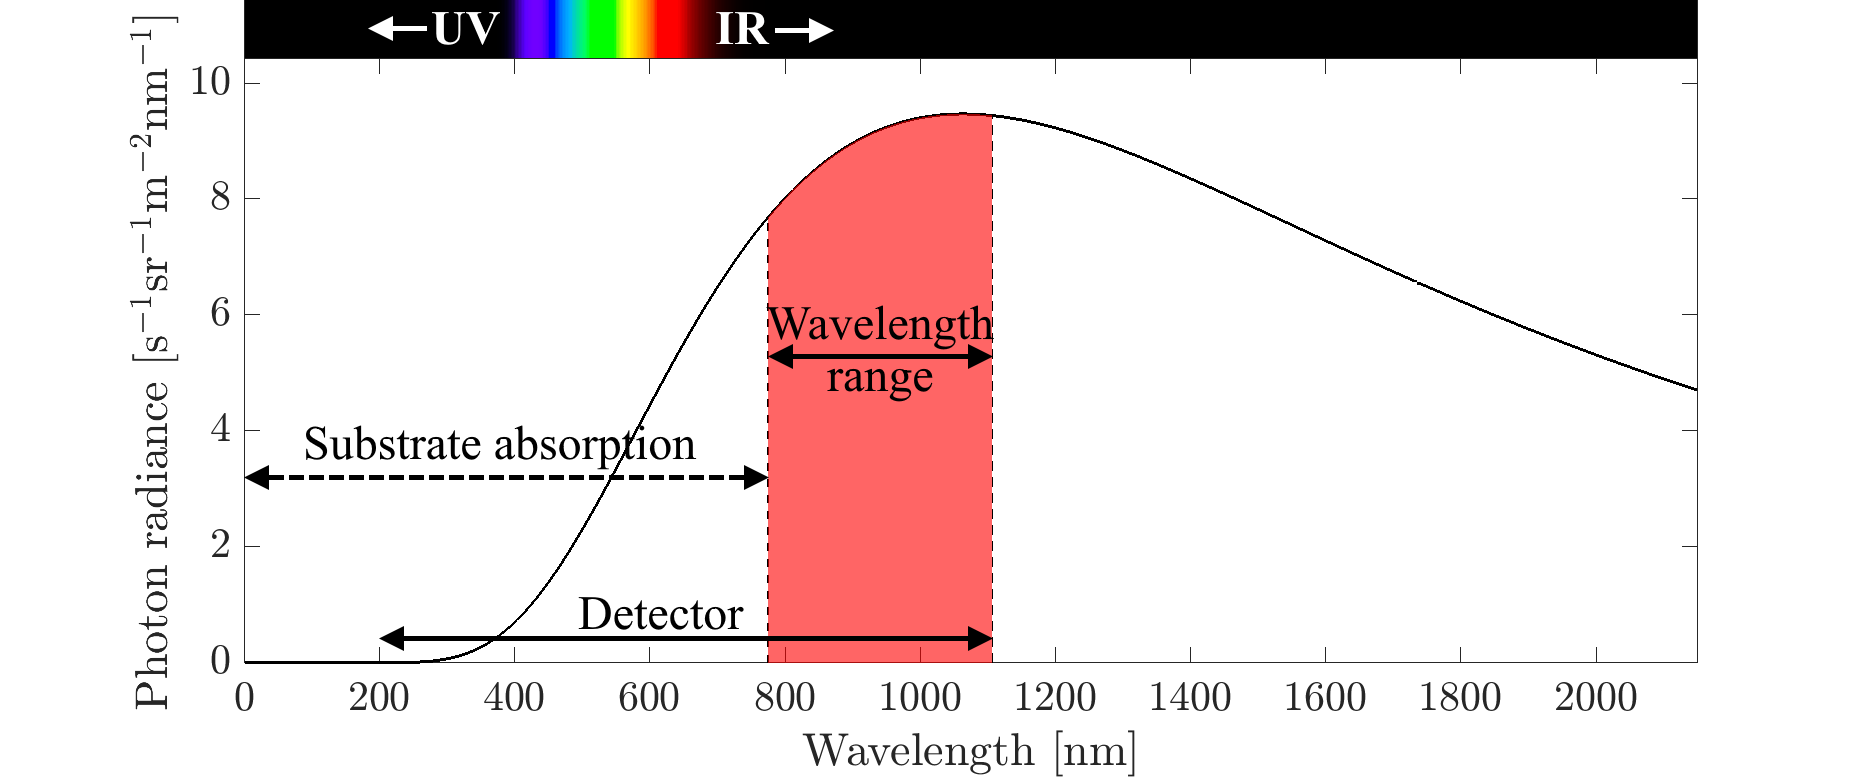
\includegraphics[width=1.0\linewidth,,trim={1.6cm 0cm 1.6cm 0cm},clip]{blackbody_photon_radiance.png}
    \caption[Graph showing the wavelength range of the near-\ac{ir} transmission microscopy setup.]{The wavelength range of the near-\ac{ir} transmission microscopy setup used in this study. The black curve is the number of photons emitted per unit wavelength per second per steradian from one square meter of a perfect black-body at a temperature of \SI{3450}{\kelvin} given by Planck's law of black-body radiation, see Eq.~\eqref{eq:planck-law}. The red area represents the photons that are transmitted through the sample and detected by the \ac{ir} camera, i.e. have an energy smaller than the bandgap of \ac{czt} (\SI{>775}{\nano\metre}),  and has an energy within the detector range of the \ac{ir}-camera (\SIrange{200}{1125}{\nano\metre}). The coloured bar above the graph illustrates at which wavelengths ultraviolet (UV), visible, and infrared (IR) radiation are found.}
    \label{fig:ir-range}
\end{figure}

%Bruker XFlash 5010 semiconductor silicon drift detector for energy dispersive spectrometers
%A Hitachi Model SU6600 Variable pressure Schottky field emission gun scanning electron microscope with a Bruker XFlash 5010 detector for the energy-dispersive X-ray spectrometer was used to find and identify defects, damage, and particles on the substrate surfaces. The \ac{sem} is capable of much higher magnifications and has a greater resolving power than the optical microscope. Hence, it can see much smaller objects in finer detail. A quantitative determination of the chemical composition of different areas and features were obtained using the Bruker Quantax Microanalysis System software.
A Hitachi Model SU6600 Variable pressure Schottky field emission gun scanning electron microscope was used to find defects, damage, and particles on the substrate surfaces. The \ac{sem} is capable of much higher magnifications and has a greater resolving power than the optical microscope. Hence, it can see much smaller features in finer detail. The \ac{sem} is equipped with a Bruker XFlash 5010 detector for the energy-dispersive X-ray spectrometer. \Ac{eds} was used to identify composition of defects, damage, and particles on the substrate surfaces. A quantitative determination of the chemical composition of different areas and features was obtained using the Bruker Quantax Microanalysis System software.

\Ac{xps} measurements were carried out with a SPECS system equipped with an \ce{Al}/\ce{Mg} twin anode XR50 X-ray source and a Riber MAC2 analyser. The \ce{Mg} anode was operated at \SI{300}{\watt} and the X-ray beam was incident at \SI{45}{\degree} with the sample normal, while emitted photoelectrons were collected in the analyser at \SI{30}{\degree}. The data was retrieved from the Riber MAC2 control unit by Cameca's Kernel 3 software, and surface composition was determined with standard methods described by \citet{moulder2000handbook} using intensity peak areas, obtained using Systat Software's PeakFit program, and elemental sensitivity factors measured experimentally on the \ac{xps} equipment at \ac{ffi} by \citet{hirsch1999x-ray}.% Or Cameca with Riber EA 150

%The \ac{xps} equipment is situated in a vacuum chamber that is attached to the \ac{mbe} machine. Samples are mounted on molybdenum blocks before they go into this machine. However, as the \ac{xps} X-ray beam diameter is as large as \SI{1}{\centi\metre}, and spectra both in the middle and along the sides of the substrates were going to be acquired, the material for the holder surrounding the substrate had to be chosen so that it did not have peaks overlapping with the elements of interest in this study. After careful considerations it was decided to make the holder from titanium, whose binding energies do not overlap with those of either \ce{Cd}, \ce{Te}, \ce{Zn}, \ce{Hg}, \ce{Al}, \ce{Si}, \ce{Cl}, \ce{S}, \ce{P}, \ce{Fe}, \ce{Br}, \ce{Cu}, \ce{O}, or \ce{C}, which are either observed in our acquired \ac{eds} spectra or found by \citet{benson2015as-received}.
%The substrate was placed in a titanium stand and secured by two titanium plates in the corners before being mounted onto a molybdenum block, and then inserted into the introduction chamber of the vacuum system before being transferred to the surface analysis chamber. The \ac{xps} data were acquired with \ce{Mg} K$\alpha$ x-ray radiation from a non-monochromatic source having an energy of \SI{1253.6}{\electronvolt}.

%With the large beam size we could only hope to see traces of impurity elements over a large area, but not locate them to specific particles or areas. Also, photoelectrons are only emitted if emitted from an atom within approximately \SI{80}{\angstrom} from the surface, so the technique can only tell us about the outermost layer of the sample. Unfortunately, something was broken on the old analyser, resulting in low signal intensity and no detection of impurities or small concentrations of elements. The ever-present oxide and carbon overlayers further decreased any small signals. Therefore, the \ac{xps} only gave information about the following elements: \ce{Te}, \ce{Cd}, \ce{O} and \ce{C}.
%Due to low count rates it was not possible to get enough statistics to detect surface impurities. Due to the low quality of the results, only substrate A was characterised using this technique.

Topographic mapping of the surfaces was performed with a Park Systems XE-100 atomic force microscope. The \ac{afm} images were recorded in non-contact mode using a Nanosensors PPP-NCHR probe with aluminium coating on the detector side. The images were obtained using a scan rate of \SI{0.2}{\hertz} and a scan size of \SI{5}{\micro\metre}. The \ac{afm} is capable of much higher depth and height resolution than the other techniques, and hence, it can be used to obtain greater detail of surface irregularities like scratches and voids.

A Perkin Elmer spectrum GX \ac{ftir} system was used to obtain transmission spectra of the substrates. The spectra present the \ac{ir} transmittance of the substrates in the wavenumber range of \SIrange{370}{5000}{\centi\metre^{-1}}. They were used to get information about the density and size of tellurium precipitates, the free carrier concentration, and the resistivity of the substrates. % to see how much light that is transmitted through the material at the different \ac{ir} wavelengths

%%=========================================
%%%=========================================
\chapter{Results and Discussion}\label{ch:results-and-discussion}
In this chapter, experimental results are presented, analysed, and discussed. In total, one (111)B substrate from vendor A (substrate A), two (111)B substrates from vendor B (substrate B and substrate B2), and one (211)B substrate from vendor A (substrate C) were investigated using bright and dark field microscopy, \ac{sem}, \ac{eds}, \ac{afm}, near-\ac{ir} transmission microscopy, and \ac{ftir}. The substrates were investigated both as-received and after surface pre-growth preparation, except substrate B2, which was not investigated as-received. As the final step, \iac{mct} film was grown on each substrate, except the shattered substrate B, and the same characterisation as for the substrates was conducted to correlate the number of defects and the type of defects in the grown \ac{mct} layer with the preparation of the substrate. \todo{The results will be summarized in tables at the end of the chapter?}
%%=========================================
\section{Surface Analysis of As-Received Substrate A}\label{sec:subAa}
% Substrate A
In previous work \citep{lauten2017characterisation}, the state-of-the-art as-received (111)B-oriented substrate A was characterised for polishing damage, defects, and residual particles using optical microscopy, \ac{sem} with \ac{eds}, and \ac{xps}. The results are reiterated in this section to better present the full scope of the study. In addition to the previously used methods, \ac{afm}, near-\ac{ir} transmission microscopy, and \ac{ftir} were used to study the as-received substrate.

\todo{Begynne med et BF bilde for å gi en ide om hvordan det ser ut?}

\begin{figure}[htbp]
    \centering
    \mySubfigure{\linewidth}{LM_DF_BZ1503ID71A_M005_centre.jpg}[fig:subAa_om_df_centre]
    \par\bigskip
    \mySubfigure{0.4525\textwidth}{LM_DF_BZ1503ID71A_M005_edge.jpg}[fig:subAa_om_df_edge]
    \hfill
    \mySubfigure{0.5225\textwidth}{LM_DF_BZ1503ID71A_M005_corner_with_skraa.jpg}[fig:subAa_om_df_corner]
    \caption[Dark field images of substrate A.]{Dark field images of substrate A captured through the optical microscope Leica DM RXA2 at three different locations on the substrate surface: \subref{fig:subAa_om_df_centre} Centre; \subref{fig:subAa_om_df_edge} edge; and \subref{fig:subAa_om_df_corner} corner.}
    \label{fig:subAa_om_df}
\end{figure}

Dark field images from the surface of substrate A at the corner, edge, and centre of the substrate, see Fig.~\ref{fig:subAa_om_df}, show that the highly polished (111)B surface was smooth and with only a few particles or morphological defects. The particle and morphological defect density was estimated to be \SI{4e2}{\centi\metre^{-2}} at the centre and \SI{1e3}{\centi\metre^{-2}} at the edges and corners of the surface of substrate A. Here the particle and morphological defect density refers to the sum of all light-scattering objects with sizes \SI{>0.5}{\micro\metre} since any features \SI{<0.5}{\micro\metre} were invisible in the dark field images. Therefore, the true morphological defect density was higher than the one estimated from these images.
% --- Measured with tolerance of 7 using ImageJ.
%       Centre: 17 partikler på 2048x1536
%       Corner: 30 partikler på 1732x1327

The substrates from vendor A were considered to be state-of-the-art \ac{czt} substrates. They were fine-polished by the vendor, and consequently, they had few surface features. This made it challenging to focus the \ac{sem} and find particles on the surface. At a magnification of $100\times$, no particles or defects could be seen, see Fig.~\ref{fig:EDX_BZ1503A_a_m001}. As a result of a higher occurrence of particles towards the edges of the substrate, it was easier to find focus near the edges. An area from the left edge of the substrate with 12 bright spots and three dark vertical lines were observed in Fig.~\ref{fig:substrateA_a2_m005}. The dark, vertical lines were carbon contamination from the \ac{sem} and was not studied further. The bright spots corresponded to an irregularity or particle on the surface. These features will be described in the following by, among other methods, high-resolution \ac{sem} images and \ac{eds} spectra.

\begin{figure}[htbp]
    \centering
    \mySubfigure{0.49\linewidth}{EDX_BZ1503A_a_m001.jpg}[fig:EDX_BZ1503A_a_m001]
    \hfill
    \mySubfigure{0.49\linewidth}{substrateA_a2_m005.jpg}[fig:substrateA_a2_m005]
    \caption[\Ac{sem} images of substrate A.]{\Ac{sem} images of the surface of substrate A taken near the left edge at \subref{fig:EDX_BZ1503A_a_m001} low ($100\times$) and \subref{fig:substrateA_a2_m005} high magnification ($3500\times$).}
    \label{fig:subA_overview}
\end{figure}
% A particle and morphological defect density of features \SI{>0.5}{\micro\metre} of \SI{4e2}{\centi\metre^{-2}} at the centre and \SI{1e3}{\centi\metre^{-2}} at the edges of the substrate was observed. Substrate A had polishing scratches that were between 10 and \SI{20}{\nano\metre} wide. In addition, pieces of residual polishing grit was found on the surface. An \ac{eds} spectrum of an agglomeration of multiple particles revealed that they were composed of alumina (\ce{Al2O3}) and silica (\ce{SiO2}) polishing grit. In addition, larger particles with size of \SI{\sim 10}{\micro\metre} on the substrate surface were observed. \Ac{eds} revealed that these particles mainly consisted of titanium.

%%=========================================
\subsection{Particles}
There were so few particles on substrate A that it was difficult to determine a density of particles on this substrate. The surface was so uniform that it was difficult to keep in focus even at high magnification. However, four different types of particles were found and identified close to the edges of substrate A, as seen in Fig.~\ref{fig:subAa_sem_w_eds}.

\begin{figure}[htbp]
    \centering
    \begin{subfigure}[t]{\textwidth}
        \caption{}\label{fig:subAa_polishing-grit}
          \begin{minipage}[c]{0.43\linewidth}
            \centering
            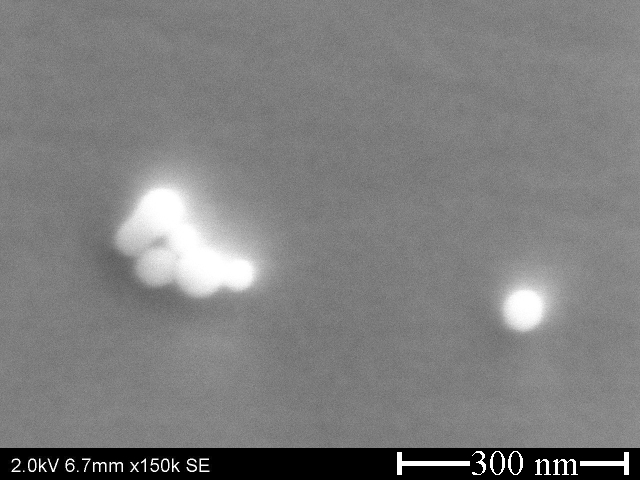
\includegraphics[width=\linewidth]{substrateA_a2_m006.jpg}
          \end{minipage}
          \hfill
          \begin{minipage}[c]{0.43\linewidth}
            \centering
            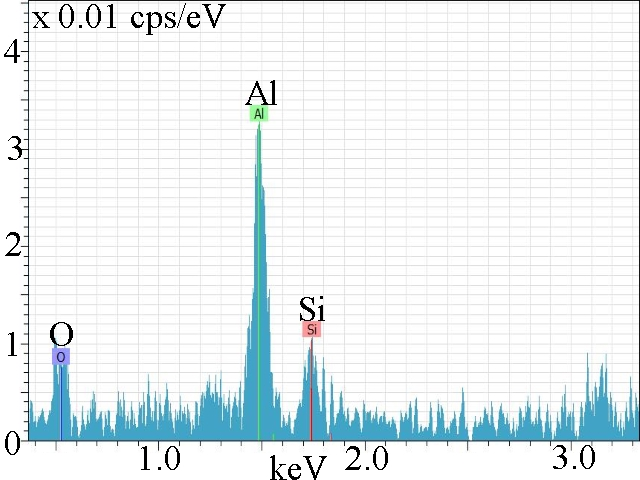
\includegraphics[width=\linewidth]{subA_eds_alumina02.jpg}
          \end{minipage}
          \begin{minipage}[c]{0.11\linewidth}
            \centering
            \atomicTable[\ce{O} &\SI{30.17}{}][\ce{Al} &\SI{21.58}{}][\ce{Ni}&\SI{14.50}{}][\ce{Cu}&\SI{10.93}{}][\ce{Fe}&\SI{9.00}{}][\ce{Si}&\SI{6.67}{}][\ce{C}&\SI{3.02}{}][\ce{Cd}&\SI{2.75}{}][\ce{Te}&\SI{1.86}{}]
          \end{minipage}
    \end{subfigure}
    \par\bigskip
    \begin{subfigure}[t]{\textwidth}
        \caption{}\label{fig:subAa_czt-particle}
          \begin{minipage}[c]{0.43\linewidth}
            \centering
            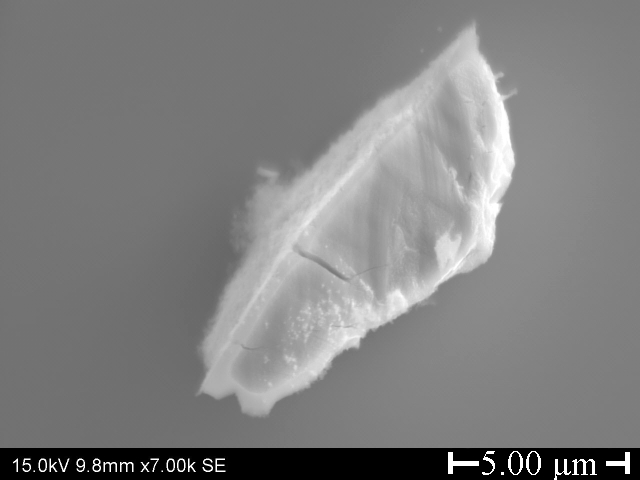
\includegraphics[width=\linewidth]{substrateA_a2_m011.jpg}
          \end{minipage}
          \hfill
          \begin{minipage}[c]{0.43\linewidth}
            \centering
            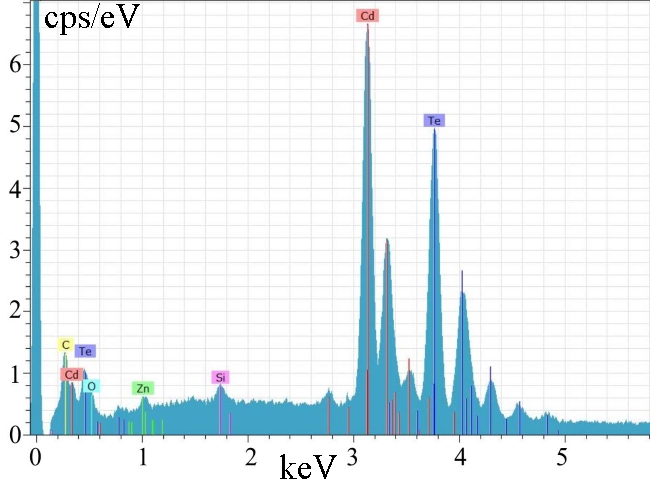
\includegraphics[width=\linewidth]{eds_subA_CZT.jpg}
          \end{minipage}
          \begin{minipage}[c]{0.11\linewidth}
            \centering
            \atomicTable[\ce{Te}&\SI{38.15}{}][\ce{Cd}&\SI{35.51}{}][\ce{C}&\SI{14.26}{}][\ce{O}&\SI{8.35}{}][\ce{Zn}&\SI{1.92}{}][\ce{Si}&\SI{1.80}{}]
          \end{minipage}
    \end{subfigure}
    \par\bigskip
    \begin{subfigure}[t]{\textwidth}
        \caption{}\label{fig:subAa_titanium-particle}
          \begin{minipage}[c]{0.43\linewidth}
            \centering
            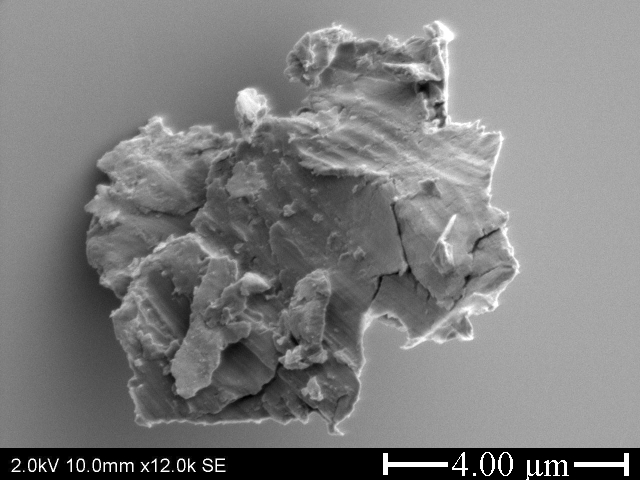
\includegraphics[width=\linewidth]{titan_sem.jpg}
          \end{minipage}
          \hfill
          \begin{minipage}[c]{0.43\linewidth}
            \centering
            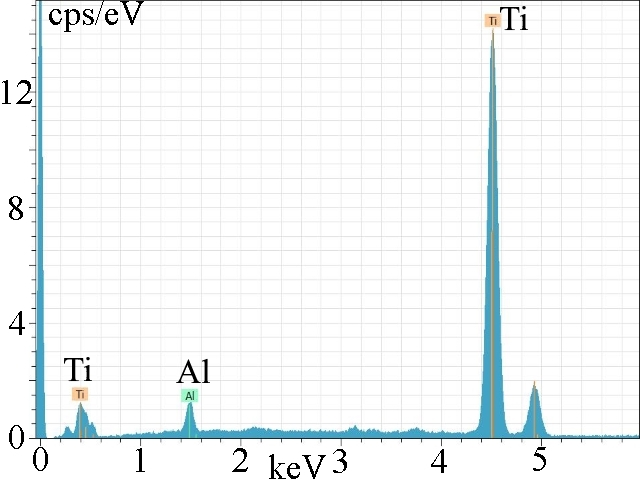
\includegraphics[width=\linewidth]{titan_eds.jpg}
          \end{minipage}
          \begin{minipage}[c]{0.11\linewidth}
            \centering
            \atomicTable[\ce{Ti}&\SI{51.69}{}][\ce{O}&\SI{16.05}{}][\ce{C}&\SI{14.91}{}][\ce{Ni} & \SI{10.96}{}][\ce{Te}&\SI{2.18}{}][\ce{Cd}&\SI{2.10}{}][\ce{Fe}&\SI{1.08}{}][\ce{Al}&\SI{0.79}{}][\ce{Si}&\SI{0.23}{}]
          \end{minipage}
    \end{subfigure}
    \caption[\Ac{sem} images, \ac{eds} spectra, and \ac{eds} atomic compositions of three different types of particles found on as-received substrate A.]{High resolution \ac{sem} images of three different types of particles found on the as-received substrate A and the corresponding \ac{eds} spectra and atomic compositions: \subref{fig:subAa_polishing-grit} Alumina (\ce{Al2O3}) polishing grit; \subref{fig:subAa_czt-particle} \aca{czt} (\ce{Cd_{0.96}Zn_{0.04}Te}) particle; and \subref{fig:subAa_titanium-particle} titanium (\ce{T}) particle.}\label{fig:subAa_sem_w_eds}
\end{figure} 


%%=====
\subsubsection{Alumina (\ce{Al2O3}) } %and Silica (\ce{SiO2}) Polishing Grit
Small, round particles of size \SI{50}{\nano\metre} were observed near the edges of substrate A, see Fig.~\ref{fig:subAa_polishing-grit}. The \ac{sem} image shows an agglomeration of particles and one single particle with a diameter of \SI{50}{\nano\metre}. The large piece was an agglomeration of the smaller ones. The corresponding \ac{eds} spectrum of the large piece revealed that the particles consisted of \ce{Al2O3}. The particles were most likely residual alumina polishing grit which are commonly used in polishing slurries \citep{benson2015as-received}.

The slurry polishes and flattens the substrate through mechanical action. The alumina particles in the slurry are suspended throughout the bulk of the medium because of the negative charges that are incorporated on the alumina particle surface and make the particles repel each other. The polishing grit appeared to be electrostatically bound to the top surface layer of the substrate.

It was easier to find polishing grit particles in close proximity to the edges of the substrate rather than in the middle. The density of the particles was therefore higher towards the edges than in the centre. Even though it was difficult to focus in the centre, the small particles would have been possible to focus on if any had been there.

The upper limit on the polishing grit density close to the edges of the substrate was estimated to be \SI{2e5}{\centi\metre^{2}}. It was not possible to get any sharp \ac{sem} images to count the density of polishing grit further in on the substrate, but it could be assumed that the density further in was at least a factor 10 less than close to the edge, as was the case for the other substrates, and hence, less than \SI{2e4}{\centi\metre^{2}}.

%%=====
\begin{comment}

    \begin{subfigure}[t]{\textwidth}
        \caption{}\label{fig:subAa_large-grit}
          \begin{minipage}[c]{0.43\linewidth}
            \centering
            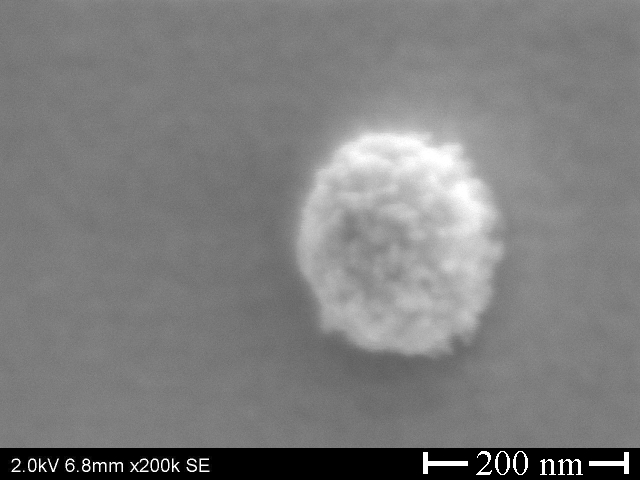
\includegraphics[width=\linewidth]{substrateA_a1_m016.jpg}
          \end{minipage}
          \hfill
          \begin{minipage}[c]{0.43\linewidth}
            \centering
            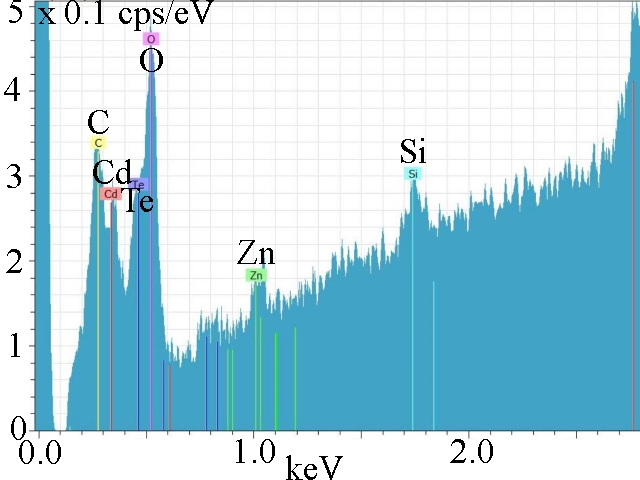
\includegraphics[width=\linewidth]{eds_subA_SiO2.jpg}
          \end{minipage}
          \begin{minipage}[c]{0.11\linewidth}
            \centering
            \atomicTable[&][&][&]
          \end{minipage}
    \end{subfigure}
    \par\bigskip
% \subref{fig:subAa_large-grit} silicon carbide (\ce{SiC}) and silica (\ce{SiO2});
\subsubsection{Silicon Carbide (\ce{SiC}) and Silica (SiO2)}
A particle with a diameter of \SI{200}{\nano\metre} is shown in Fig.~\ref{fig:subAa_large-grit} with the corresponding \ac{eds} spectrum. This particle was considerably larger and had a rougher surface than the more frequently observed \SI{50}{\nano\metre} particles that were found to be residual polishing grit. The \ac{eds} spectrum of the particle revealed that the particle consisted of \ce{Si}, \ce{C}, and \ce{O}, which indicated that this particle could be residual \ce{SIO2} polishing grit, \ce{SiC} polishing grit, or an agglomeration of both. \todo{Finn atomprosent for å avgjøre. SiC eller SiO2? Hvor kommer C fra hvis bare SiO2?}
\end{comment}

%%=====
\subsubsection{CZT}
Particles with size \SI{>5}{\micro\metre} were observed primarily near the edges of substrate A. Fig.~\ref{fig:subAa_czt-particle} shows a particle that was \SI{13}{\micro\metre} long and \SI{5}{\micro\metre} wide. A comparison between the corresponding \ac{eds} spectrum of the particle and the substrate surface spectrum revealed that the particle consisted of the same material as the underlying substrate. It could be debris from the cutting and polishing of the substrate and the making of bevelled edges by the vendor.


%%=====
\subsubsection{Titanium}
Particles with sharp edges and sizes of \SI{>5}{\micro\metre} were observed in the upper left corner of the substrate. The particles appeared darker than the \ac{czt} particles in \ac{sem} and with more edges. Fig.~\ref{fig:subAa_titanium-particle} shows a particle that was \SI{8}{\micro\metre} long and \SI{4}{\micro\metre} wide. The corresponding \ac{eds} spectrum of the particle revealed that the particle mainly consisted of titanium. The sharp edges indicate that the particle had not not been used as polishing grit because the edges had been rounded in that case. Unfortunately, these particles probably had settled on the substrate during the study. A new substrate holder was made for \ac{xps} measurements out of titanium in the machine shop. When mounting the substrate in the holder with a screw, some titanium particles were made. However, they were confined to a small area in the upper left corner of the substrate. \Ac{sem} and \ac{eds} measurements of particles from the \ac{xps} holder, collected with an adhesive carbon tab, confirms that the same type of titanium particles was found on the \ac{xps} holder. %This fact, shows how important it is to clean the equipment carefully before use. %see Fig.~\ref{fig:subAa_titanium}


%%=========================================

\subsection{Surface Scratches and Roughness}
The as-received surface of substrate A was carefully polished by the vendor, as seen in Fig.~\ref{fig:subAa_scratches}. The surface scratches most likely had shallow depth since they could not be observed in the dark field images of substrate A, see Fig.~\ref{fig:subAa_om_df}.

\begin{figure}[htbp]
    \centering
    %\subfigure[High resolution SEM at SEM image at a magnification of 80000$\times$.]{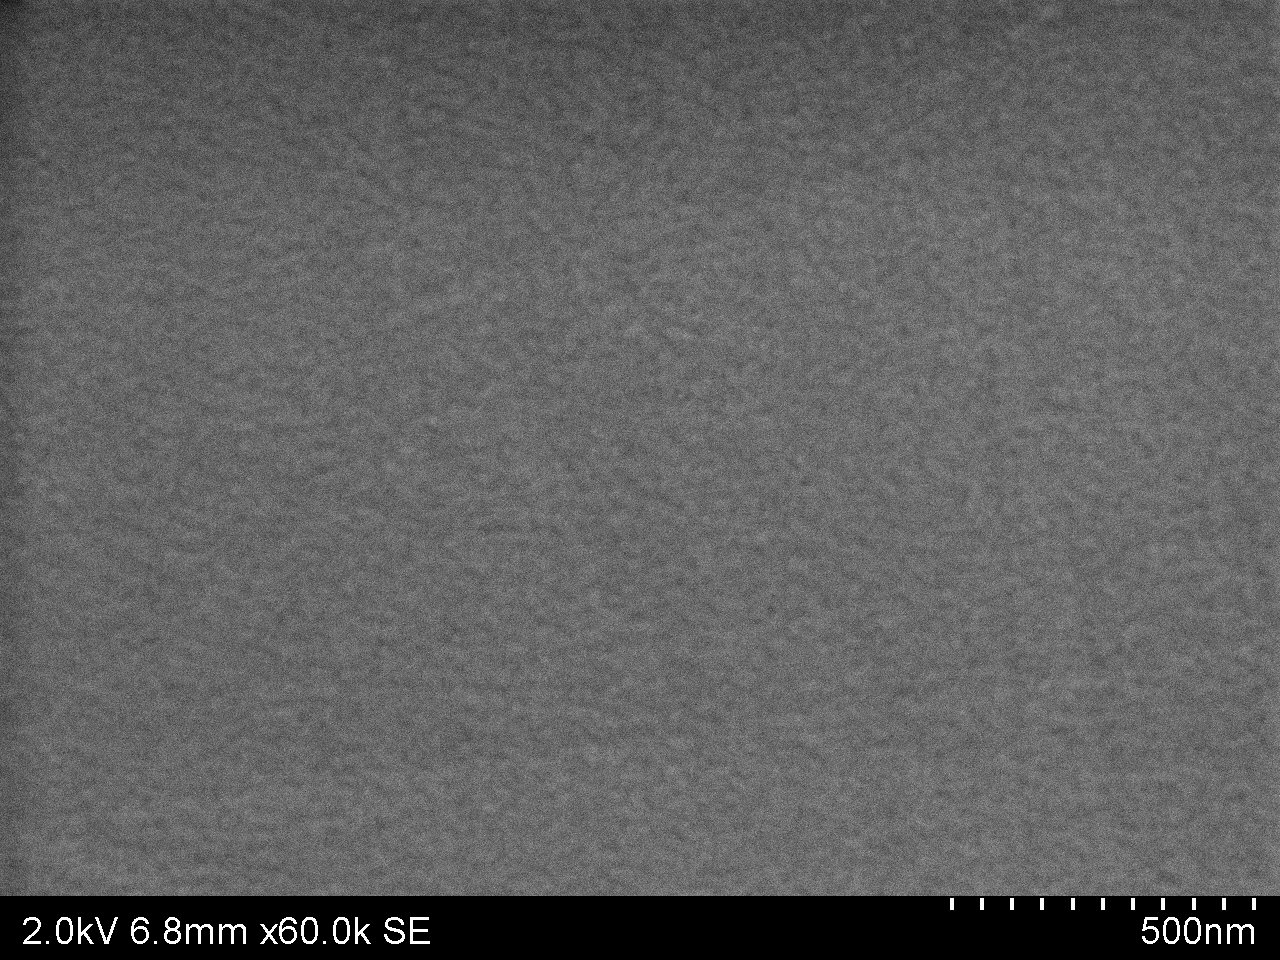
\includegraphics[width=0.48\linewidth]{substrateA_a2_m003.jpg}\label{fig:substrateA_a2_m003}}
    %\quad
    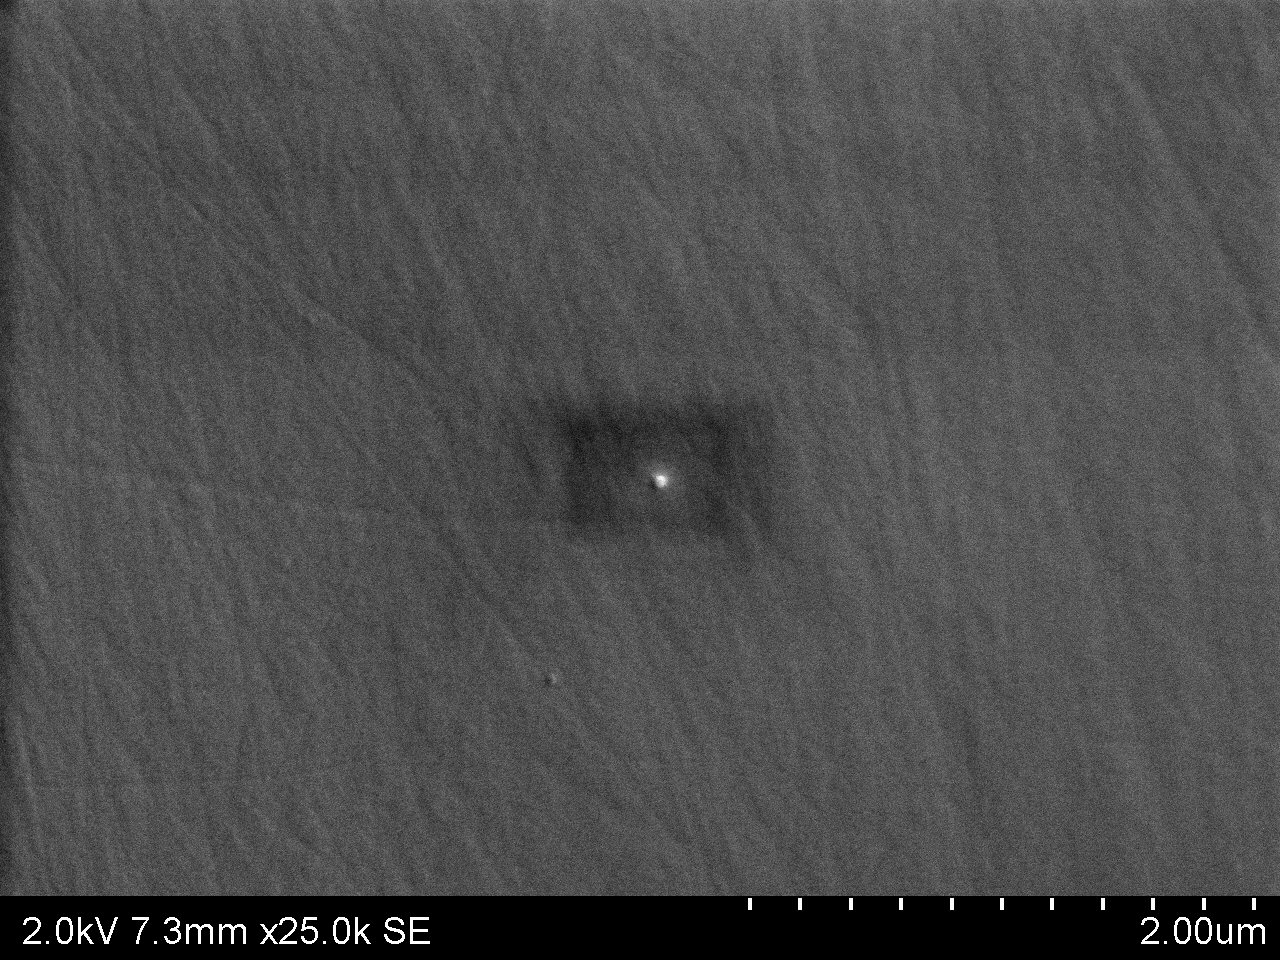
\includegraphics[width=0.6\linewidth]{substrateA_a1_m011.jpg}
    \caption[\Ac{sem} image of surface scratches on substrate A.]{High resolution \ac{sem} image of the surface of substrate A. The dark square was carbon deposited on the surface while focusing the beam at a higher magnification.}\label{fig:subAa_scratches}
    \label{fig:SEM_A_surface}
\end{figure}

The as-received substrate A was characterised for surface topography by \ac{afm}. Images of $\SI{5}{\micro\metre}\times\SI{5}{\micro\metre}$ areas were taken at three different locations on the substrate surface: near the centre, near the upper edge, and near the upper left corner, as seen in Fig.~\ref{fig:subAa_afm}. The \ac{rms} roughness of substrate A was \SI{\sim0.3}{\nano\metre} at both the centre and around the edges, while it was \SI{\sim0.4}{\nano\metre} at the corner. This indicates the absence of large scratches. The typical surface scratches were between \SIrange{10}{20}{\nano\metre} wide and \SI{1}{\nano\metre} deep. While the largest polishing scratches were \SI{0.2}{\micro\metre} wide and \SI{5}{\nano\metre} deep.

\begin{figure}[htbp]
    \centering
    \begin{subfigure}[c]{0.032\linewidth}
        \label{fig:subAa_afm_scale}\captionsetup{list=no}
        
\includegraphics[width=\linewidth]{subAa_afm_scale.png}
    \end{subfigure}
    \hfill
    \mySubfigure{0.3\linewidth}{subAa_afm_centre.png}[fig:subAa_afm_centre]
    \hfill
    \mySubfigure{0.3\linewidth}{subAa_afm_upperedge.png}[fig:subAa_afm_edge]%0,26
    \hfill
    \mySubfigure{0.3\linewidth}{subAa_afm_upperleftcorner.png}[fig:subAa_afm_corner]%0,26
    \caption[\Ac{afm} of as-received substrate A.]{\Ac{afm} measurements of the as-received substrate A. Images of $\SI{5}{\micro\metre}\times\SI{5}{\micro\metre}$ areas are taken at three different locations on the substrate surface: \subref{fig:subAa_afm_centre} near the centre, \ac{rms} roughness \SI{0.31}{\nano\metre}; \subref{fig:subAa_afm_edge} near the upper edge, \ac{rms} roughness \SI{0.30}{\nano\metre}; and \subref{fig:subAa_afm_corner} near the upper left corner, \ac{rms} roughness \SI{0.41}{\nano\metre}.}\label{fig:subAa_afm}
\end{figure} % AFM, substrate A, as-received.

%%=========================================
%\section{Near-IR of As-Received Substrate A}

%%=========================================
\subsection{Impurity Analysis -- XPS}

\Ac{xps} analysis was performed on the as-received substrate A to determine the composition of the outermost layers of the substrate (\SI{\sim 80}{\angstrom}). The centre of the $\SI{30}{\milli\metre}\times\SI{30}{\milli\metre}$ \ac{czt} wafer was analysed using \ac{xps}. With the large beam size of \SI{1}{\centi\metre}, it should be possible to see traces of impurity elements over a large area, but not locate them to specific particles or small areas. Unfortunately, something was broken on the old analyser, resulting in low signal intensity and no detection of impurities or small concentrations of elements. The ever-present oxide and carbon overlayers further decreased any small signals. Therefore, the XPS only provided information about the following elements: \ce{Te}, \ce{Cd}, \ce{O}, and \ce{C}, see Fig.~\ref{fig:xps_spectra}. The reason for not performing \ac{xps} analysis on substrate B was that it would not be possible to detect the presence of impurities or small concentrations of elements with the \ac{xps} equipment at hand.

\begin{figure}[htbp]
    \centering
    \mySubfigure{0.49\linewidth}{xps_Te3d.png}[fig:xps_Te3d]
    \hfill
    \mySubfigure{0.49\linewidth}{xps_Cd3d.png}[fig:xps_Cd3d]
    \par\bigskip
    \mySubfigure{0.49\linewidth}{xps_O1s.png}[fig:xps_O1s]
    \hfill
    \mySubfigure{0.49\linewidth}{xps_C1s.png}[fig:xps_C1s]
    \caption[\Ac{xps} spectra from substrate A.]{\Ac{xps} spectra from substrate A that displays the number of detected electrons (counts) as a function of their corresponding binding energy, $E_\mathrm{B}$ (\SI{}{\electronvolt}). The spectra were acquired using the \ce{Mg} anode. The peaks in the spectrum were: \subref{fig:xps_Te3d} \ce{Te} 3d with extra peaks due to tellurium oxide; \subref{fig:xps_Cd3d} \ce{Cd} 3d; \subref{fig:xps_O1s} \ce{O} 1s; and \subref{fig:xps_C1s} \ce{C} 1s.}
    \label{fig:xps_spectra}
\end{figure}
 
The atomic concentrations were calculated using Eq.~\eqref{eq:xps_concentration} with intensity peak areas and the following experimentally measured atomic sensitivity factors, determined earlier at \ac{ffi} \citep{hirsch1999x-ray}: \ce{Cd} 3d\textsubscript{5/2} (0.56), \ce{Te} 3d\textsubscript{5/2} (1.00), \ce{O} 1s (0.13), and \ce{C} 1s (0.05). Table~\ref{tab:xps_results} displays the results of the \ac{xps} analysis of substrate A. \ce{Cd_{0.96}Zn_{0.04}Te} should consist of \SI{48}{\atomic\percent} cadmium, \SI{2}{\atomic\percent} zinc and \SI{50}{\atomic\percent} tellurium, but zinc was not detected and the atomic concentration of \ce{Cd} was only \SI{75}{\percent} of that of \ce{Te}, it should be \SI{96}{\percent}. The higher than expected \ce{Te} concentration can be explained by the formation of a \ce{Te} oxide layer on the surface. By inserting the ratio between \ce{Te} in \ce{Cd_{1-y}Zn_yTe} signal and \ce{Te} in \ce{TeO} signal of \SI{1.3}{} into Eq.~\eqref{eq:signal_ratio}, the \ce{Te} oxide layer thickness was calculated to be \SI{0.96}{\nano\metre}. An atomic concentration of $23.5$ at.\% carbon was found, which can be explained by an overlayer of carbon. %\todo{How thick?}

\begin{table}[htbp]
    \centering
    \caption[XPS analysis of the as-received substrate A.]{Results from the \ac{xps} analysis at the centre of the $30\times30$ \SI{}{\milli\metre} as-received (111)B \ce{CdZnTe} substrate A (atomic concentration \%).}\label{tab:xps_results}
    \begin{tabu} to 1.0\textwidth { X[1,c] X[1,c] X[1,c] X[1,c] X[1,c] }
    \hline
        %\textbf{$X$} (\SI{}{\milli\metre}) &  \textbf{$Y$} (\SI{}{\milli\metre}) & \textbf{\ce{Cd} (\SI{}{\atom\centi\metre^{-2}})} & \textbf{\ce{Te} (\SI{}{\atom\centi\metre^{-2}})} & \textbf{\ce{O} (\SI{}{\atom\centi\metre^{-2}})} & \textbf{\ce{C} (\SI{}{\atom\centi\metre^{-2}})} & \textbf{\ce{Te} oxide thickness (\SI{}{\nano\metre})}\\
        \textbf{\ce{Cd}}\newline(at.\%) & \textbf{\ce{Te}}\newline(at.\%) & \textbf{\ce{O} }\newline(at.\%) & \textbf{\ce{C}}\newline(at.\%) & \textbf{\ce{Te} oxide thickness}\newline(\SI{}{\nano\metre})\\
        \hline
         \SI{18.8}{} & \SI{25.1}{} & \SI{32.6}{} & \SI{23.5}{} & \SI{0.96}{} \\
         \hline
    \end{tabu}
\end{table}
%\mycomment{Add PeakFit-figures. Describe satellite peaks.}

%%=========================================
\subsection{Impurity Analysis -- EDS}
Since the \ac{xps} equipment did not detect small concentrations of elements, \ac{eds} was used to get a quantitative analysis of the chemical composition of the substrate. The spectra were taken using an accelerating voltage of \SI{10.0}{\kilo\volt} to ensure an electron energy larger than the peaks of interest, but still limited in order to not fet too deep into the sample, a large probe current to maximise the throughput, and a live acquisition time of \SI{1200}{\second} to get reliable statistics and less noise. The resulting \ac{eds} spectrum from the centre of the substrate can be seen in Fig.~\ref{fig:subAa_eds_centre}. %an extraction voltage of \SI{2.00}{\kilo\volt} to get 

\begin{figure}[htbp]
    \centering
    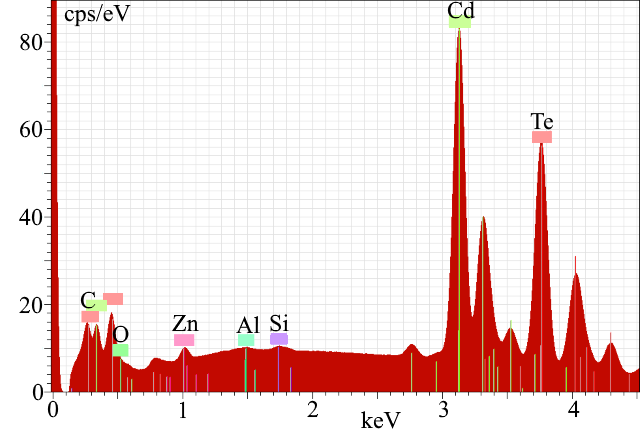
\includegraphics[width=0.7\linewidth]{subAa_eds_centre.png}
    \caption[\Ac{eds} spectrum from the centre of the as-received substrate A.]{\Ac{eds} spectrum from a $\SI{1270}{\micro\metre}\times\SI{890}{\micro\metre}$ area in the centre of the as-received substrate A.}
    \label{fig:subAa_eds_centre}
\end{figure}

The spectra were collected from surface areas of $\SI{1270}{\micro\metre}\times\SI{890}{\micro\metre}$. The electron interaction depth was calculated by the Quantax software to be \SI{0.4}{\micro\metre}. That means that characteristic X-rays from elements as far in as \SI{0.4}{\micro\metre} below the surface were detected. In comparison, the \ac{xps} detected the electrons that escaped from the outermost \SI{\sim10}{\nano\metre}. Hence, \ac{eds} was not as surface sensitive and more than just the top surface layer was probed. This is part of the reason for the difference in the atomic concentrations between the \ac{xps} and \ac{eds} results for substrate A. The observed silica and alumina particles had a diameter of about \SI{50}{\nano\metre}. Hence, one monolayer of these would cover \SI{\sim12.5}{\percent} of the interaction volume, although a little more of the signal.

The \ac{eds} surface analysis identified the following elements: \ce{Cd}, \ce{Te}, \ce{Zn}, \ce{Al}, \ce{Si}, \ce{C}, and \ce{O}, as seen in Table~\ref{tab:subAa_eds_analysis}. The relative concentrations of \ce{Cd}, \ce{Zn}, and \ce{Te} had an error of less than one percentage point from the expected value of \SI{48}{\atomic\percent} cadmium, \SI{2}{\atomic\percent} zinc, and \SI{50}{\atomic\percent} tellurium. The \ac{eds} spectrum shown in Fig.~\ref{fig:subAa_polishing-grit} demonstrates that some of the aluminium contamination came from the residual \ce{Al2O3} polishing grit. The silicon contamination could come from residual \ce{SiO2} polishing grit, but future \ac{eds} measurements are required to confirm this hypothesis. Silicon and alumina were detected in close proximity to the centre as well as near the edges and corners. This indicates that the polishing grit was not exclusively near the edges an corners. %\todo{Kan du si noe om density ut fra dette?}%Substrate A had a smaller atomic concentration of \ce{O} than substrate B, which indicates that the tellurium oxide layer on substrate A was thinner than that on substrate B. The \ce{Al} and \ce{Si} contamination found in the \ac{eds} analysis for both substrate A and substrate B was coming from residual \ce{Al2O3} and \ce{SiO2} polishing grit respectively.

\begin{table}[htbp]
    \centering
    \caption[\Ac{eds} impurity analysis of the as-received substrate A.]{Results of the \ac{eds} impurity analysis at three different locations on the $\SI{30}{\milli\metre}\times\SI{30}{\milli\metre}$ as-received (111)B \ac{czt} substrate A (atomic concentration \%). The X-ray signal was acquired from a $\SI{1270}{\micro\metre}\times\SI{890}{\micro\metre}$ area near the centre, upper edge, and upper left corner.}\label{tab:subAa_eds_analysis}
    \begin{tabu} to 1.0\textwidth { X[1.85,r] X[1.125,c] X[1.125,c] X[1.125,c] X[1.125,c] X[1.125,c] X[1.125,c] X[1.125,c] }
    \hline
         & \textbf{\ce{Te}} (at.\%) & \textbf{\ce{Cd}} (at.\%) & \textbf{\ce{Zn}} (at.\%) & \textbf{\ce{Al} } (at.\%) & \textbf{\ce{Si}} (at.\%) & \textbf{\ce{C}} (at.\%) & \textbf{\ce{O}} (at.\%) \\ % \textbf{$X$} (\SI{}{\milli\metre}) &  \textbf{$Y$} (\SI{}{\milli\metre})
        \hline
        Near centre & \SI{46.14}{} & \SI{45.60}{} & \SI{1.90}{} & \SI{0.21}{} & \SI{0.51}{} & \SI{4.97}{} & \SI{0.68}{} \\ 
        Near edge  & \SI{45.94}{} & \SI{45.32}{} & \SI{1.98}{} & \SI{0.19}{} & \SI{0.45}{} & \SI{5.34}{} & \SI{0.78}{} \\
        Near corner & \SI{46.05}{} & \SI{45.46}{} & \SI{1.89}{} & \SI{0.40}{} & \SI{0.51}{} & \SI{4.95}{} & \SI{0.73}{} \\
         \hline
    \end{tabu}
\end{table}
%%========================================
% FTIR transmission spectra.
\subsection{IR Characterisation}

\Ac{ftir} transmission spectra were recorded from an $11\times11$ grid on the as-received substrate A. The grid points were placed \SI{2.0}{\milli\metre} from the edge and had \SI{2.6}{\milli\metre} between nearest neighbours. All but four measurements had an \ac{ir} transmittance between \SI{62}{\percent} and \SI{67}{\percent} in the wavenumber range between \SI{1000}{\centi\metre^{-1}} and \SI{5000}{\centi\metre^{-1}}, see Fig.~\ref{fig:subAa_ftir_spectra}. The spikes near $k=\SI{4500}{\centi\metre^{-1}}$ and $k=\SI{5000}{\centi\metre^{-1}}$ were an artefact of the \ac{ftir} instrument and should not be considered. A map of the transmission at $k=\SI{500}{\centi\metre^{-1}}$ can be seen in Fig.~\ref{fig:subAa_ftir_map_500cm-1}.

\begin{figure}[htbp]
    \centering
    \mySubfigure{0.60175438596\linewidth}{subAa_121_ftir_spectra.png}[fig:subAa_ftir_spectra]
    \hfill
    \mySubfigure{0.37824561403\linewidth}{subAa_121_ftir_transmission_at_k500cm-1.png}[fig:subAa_ftir_map_500cm-1]
    \caption[\Ac{ftir} measurements of the as-received substrate A.]{\Ac{ftir} measurements recorded from a $11\times11$ grid on the as-received $\SI{30}{\milli\metre}\times\SI{30}{\milli\metre}$ (111)B-oriented substrate A: \subref{fig:subAa_ftir_spectra} Transmission spectra; \subref{fig:subAa_ftir_map_500cm-1} transmission map at wavenumber $k=\SI{500}{\centi\metre^{-1}}$ showing the transmittance $T$ in percentage of incoming light at each grid point. The spikes near $k=\SI{4500}{\centi\metre^{-1}}$ and $k=\SI{5000}{\centi\metre^{-1}}$ were artefacts of the \ac{ftir} instrument.}
\end{figure}

The two factors that are primarily responsible for the reduction in \ac{ir} transmittance of \ac{czt} are free carrier absorption and scattering from precipitates \citep{yadava1994precipitation}. \citet{yujie2004infrared} used the transmittance at the wavenumbers $\SI{1000}{\centi\metre^{-1}}$ ($T_{1000}$) and $\SI{5000}{\centi\metre^{-1}}$ ($T_{5000}$), and the ratio of $T_{1000}$ to $T_{5000}$ to determine which of the two mechanisms that were most significant. Their analysis provided a qualitative determination of the density and size of \ce{Te} precipitates, the free carrier concentration, and the resistivity for \ac{czt} substrates. %\todo{Espen: Dislokasjoner og ruhet vil også senke transmisjon.}

Almost all the spectra from substrate A had values of $T_{5000}$ between \SIrange{63}{67}{\percent}, $T_{1000}$ between \SIrange{62}{64}{\percent}, and $T_{1000}/T_{5000}$ approached one from below. Following the analysis of \citeauthor{yujie2004infrared}, a \ac{czt} substrate with these parameters is free from precipitates and has a low free carrier concentration. Combined with the extremely low particle density, it does indeed seem that the quality of this substrate, as-received, is very good. %and had resistivity that exceeded \SI{e6}{\ohm\centi\metre}.%\todo{Why?}

\begin{figure}[htbp]
    \centering
    \mySubfigure{0.49\linewidth}{unknown.png}[fig:subAa_nirt_surface]
    \hfill
    \mySubfigure{0.49\linewidth}{unknown.png}[fig:subAa_nirt_inside]
    \caption[Near-\ac{ir} microscopy images pf \ce{Te} precipitates in substrate A.]{Near-\ac{ir} microscopy images pf \ce{Te} precipitate density and distribution near the centre of the $\SI{30}{\milli\metre}\times\SI{30}{\milli\metre}$ (111)B-oriented substrate A. Image area is $\SI{}{\micro\metre}\times\SI{}{\micro\metre}$. \subref{fig:subAa_nirt_surface} The (111)B surface; \subref{fig:subAa_nirt_inside} \SI{\sim}{\micro\metre} below the (111)B surface.}\label{fig:subAa_nirt}
\end{figure}

%\ce{Te} precipitate/inclusion density \SI{>10}{\micro\metre} = \SI{2.8e3}{\centi\metre^{-3}}. Typical \ce{Te} precipitate/inclusion density in state-of-the-art \ac{czt} is \SI{\sim2e6}{\centi\metre^{-3}}.

%\todo{Hossain 2008 fine Ir bilder ligner på våre}

\begin{comment}\todo{}
Mange artikler i denne katalogen: G:\Brukere\ESg\papers\CMT\CdZnTe

se spesielt på 
-	figurer i »CZT inclusions Belas 2008»
-	CZT substrates Japan Energy (de som lager våre subs)
-	Fig 1 i Defects in CZT. Hossain-2015

\end{comment}

%%========================================

\clearpage
%%=========================================
\section{Surface Analysis of As-Received Substrate B}\label{sec:subBa}
% Substrate B
Substrate B was from an alternative source (vendor B) and had only been roughly polished after being sliced from a bulk crystal. In previous work \citep{lauten2017characterisation}, the as-received (111)B-oriented substrate B was characterised for polishing damage, defects, and residual particles using optical microscopy and \ac{sem} with \ac{eds}. The results are reiterated in this section to better present the full scope of the study. In addition to the previously used methods, \ac{afm}, near-\ac{ir} transmission microscopy, and \ac{ftir} were used to study the as-received substrate.

\todo{BF image?}

The surface of the as-received substrate B looked completely different from that of the as-received substrate A. Fig.~\ref{fig:subBa_om_df} shows typical dark field images from the surface of substrate B at the corner, edge, and centre of the substrate. There were polishing scratches in all directions and with varying width covering the surface of substrate B. Particles and morphological defects with both small (\SIrange{0.5}{5}{\micro\metre}) and large (\SIrange{5}{50}{\micro\metre}) diameter were present on the surface. By counting the number of bright spots in the dark field image, the density of particle and morphological defects with features \SI{>0.5}{\micro\metre} was estimated to be \SI{1e5}{\centi\metre^{-2}}, both at the centre and edges of the surface of substrate B.
% --- Measured with tolerance of 10 using ImageJ. One pixel are 2250/2048 um.
%       Centre: 5739 partikler på 2048x1536 --> 151151 particles per cm^2
%       Edges: 3927 partikler på 1877x1522 --> 113888 particles per cm^2
%       Corner: 5327 partikler på 1848x1486 --> 158000 particles per cm^2

\begin{figure}[htbp]
    \centering
    \mySubfigure{\linewidth}{LM_DF_C389523A_M005_centre.jpg}[fig:subBa_om_df_centre]
    \par\bigskip
    \mySubfigure{0.49\linewidth}{LM_DF_C389523A_M005_centreEdge.jpg}[fig:subBa_om_df_edge]
    \hfill
    \mySubfigure{0.49\linewidth}{LM_DF_C389523A_M005_corner.jpg}[fig:subBa_om_df_corner]
    \caption[Dark field images of substrate B.]{Dark field images of substrate B captured through the optical microscope Leica DM RXA2 at the \subref{fig:subBa_om_df_centre} centre; \subref{fig:subBa_om_df_edge} edge; and \subref{fig:subBa_om_df_corner} corner of the substrate.}
    \label{fig:subBa_om_df}
\end{figure}

The difference between substrate A and substrate B was significant. Substrate B had a density of particles and morphological defects that was 100-1000 times larger than on substrate A. A large part of this can presumably be explained by the more thorough surface preparation that substrate A had been subjected to. Substrate A had a final polishing and an etch before it was delivered, while substrate B was roughly polished and particles on the surface had not been removed.

A comparison between the dark field image and a \ac{sem} image of the same area of substrate B, as seen in Fig.~\ref{fig:LM_SEM_C3895}, reveals that the brightest spots in the dark field image are from cavities in the substrate surface and that particles as small as \SI{0.5}{\micro\metre} can be seen in the dark field image. The dark stains, on the other hand, were not visible in the dark field image. This indicates that the dark stains do not have sharp edges or other pointy features.

\begin{figure}[htbp]
    \centering
    %\mySubfigure[Dark field optical microscope image.]{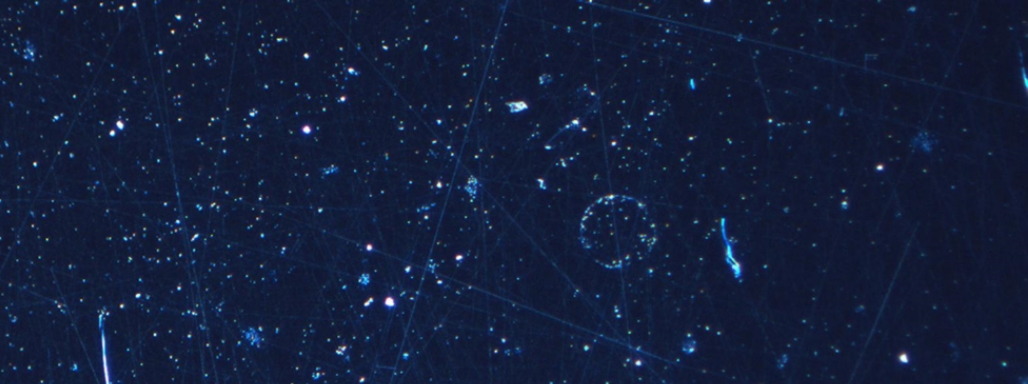
\includegraphics[width=1\linewidth]{C-3895-23A_centre_LM.jpg}\label{fig:C-3895-23A_centre_LM}}
    %\mySubfigure[SEM image at a magnification of 60$\times$.]{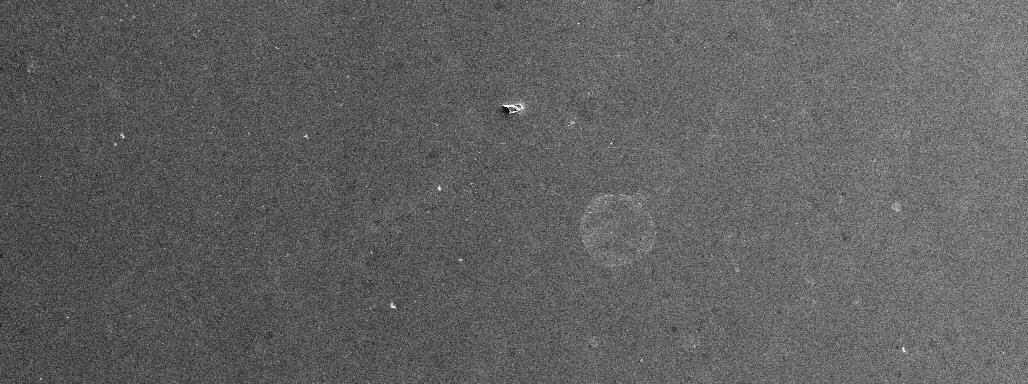
\includegraphics[width=1\linewidth]{C-3895-23A_centre_SEM.jpg}\label{fig:C-3895-23A_centre_SEM}}
    \mySubfigure{0.36\linewidth}{C-3895-23A_edge_LM_500_overview.jpg}[fig:C-3895-23A_edge_LM_500_overview]
    \hfill
    \mySubfigure{0.60\linewidth}{C-3895-23A_edge_SEM_500_overview.png}[fig:C-3895-23A_edge_SEM_500_overview]
    \caption[Comparison of dark field microscopy and \ac{sem} images.]{Comparison of \subref{fig:C-3895-23A_edge_LM_500_overview} a dark field microscopy image captured through the optical microscope Leica DM RXA2 and \subref{fig:C-3895-23A_edge_SEM_500_overview} \iacf{sem} image taken at the same location on the as-received substrate B as the dark field image.}
    \label{fig:LM_SEM_C3895}
\end{figure}

%A \ac{sem} image mapping of substrate B was performed at points in a grid of $11\times11$ grid points. The distance between neighbouring points was \SI{2.60}{\milli\metre} and the distance from the edge to the outer points was \SI{2.00}{\milli\metre}. A low magnification \ac{sem} image (60$\times$) and a higher magnification image (500$\times$) were acquired at every grid point. %This mapping will be used in future studies of substrate B when correlation between defect density and preparation methods is going to be measured.

%A particle and morphological defect density of features \SI{>0.5}{\micro\metre} of \SI{1e5}{\centi\metre^{-2}} at both the centre and at the edges of the substrate was observed. Substrate B had polishing scratches that were between 10 and \SI{100}{\nano\metre} wide. A large amount of voids with sizes ranging from \SI{5}{} to \SI{100}{\micro\metre} were observed on the surface of substrate B. 

%Most of the particles \SI{>1}{\micro\metre} on the surface of substrate B were \ce{CdZnTe} particles with lengths of between \SI{50}{} and \SI{100}{\micro\metre} that could be debris from the cutting of the substrate, but some carbon based particles was also observed with lengths of \SI{25}{\micro\metre}. Most of the particles \SI{<1}{\micro\metre} on the surface of substrate B were residual \ce{Al2O3} and \ce{SiO2} polishing grit with diameter of between \SI{50}{} and \SI{100}{\nano\metre}.  In addition, iron particles, which could be possible remainders of polishing slurry, and particles containing \ce{Na} and \ce{Cl}, which could be possible remainders of polishing slurry cleaner, were observed on the surface of substrate B.

%%=========================================
%\section{Particles and Defects on Substrate B}

Fig.~\ref{fig:C-3895-23A_F08_x060} shows a \ac{sem} image from the centre of substrate B, taken at low magnification (60$\times$). There were some bright stains at the top of the image, a dark spot down in the right corner, and several bright spots distributed over the surface. A \ac{sem} image at the same position at magnification 500$\times$, shown in Fig.~\ref{fig:C-3895-23A_F08_x500}, revealed the existence of surface scratches, dark stains of different sizes, and some even smaller bright spots on the surface. These features will be described in the following by, among other methods, \ac{sem} images at even higher magnification.

\begin{figure}[htbp]
    \centering
    \mySubfigure{0.49\linewidth}{C-3895-23A_F08_x060.png}[fig:C-3895-23A_F08_x060]
    \hfill
    \mySubfigure{0.49\linewidth}{C-3895-23A_F08_x500.png}[fig:C-3895-23A_F08_x500]
    \caption[\Ac{sem} images of a typical area in the middle of substrate B.]{\Ac{sem} images of a typical area in the middle of substrate B at \subref{fig:C-3895-23A_F08_x060} $60\times$ magnification; and \subref{fig:C-3895-23A_F08_x500} $500\times$ magnification.}
    \label{fig:SEM_C389523_overview}
\end{figure}

\subsection{Particles and Surface Features}

Seven different types of particles and surface features were observed on the surface of substrate B. These seven can be seen in Fig.~\ref{fig:subBa_sem_w_eds}.
%\mySubfigure[SEM.]{0.44\linewidth}{C-3895-23_09_m001.jpg}
    %\mySubfigure[SEM.]{0.44\linewidth}{C-3895-23A_edx7_m002.jpg}
    %\mySubfigure[SEM.]{0.44\linewidth}{C-3895-23A_edx7_m003.jpg}
\begin{figure}[htbp]
    \centering
    \begin{subfigure}[t]{\textwidth}
        \caption{}\label{fig:subBa_polishing-grit_alumina}
          \begin{minipage}[c]{0.43\linewidth}
            \centering
            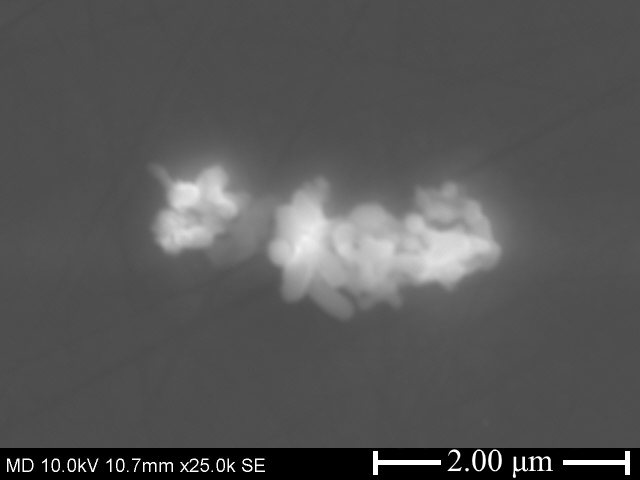
\includegraphics[width=\linewidth]{alumina02_sem.png}
          \end{minipage}
          \hfill
          \begin{minipage}[c]{0.43\linewidth}
            \centering
            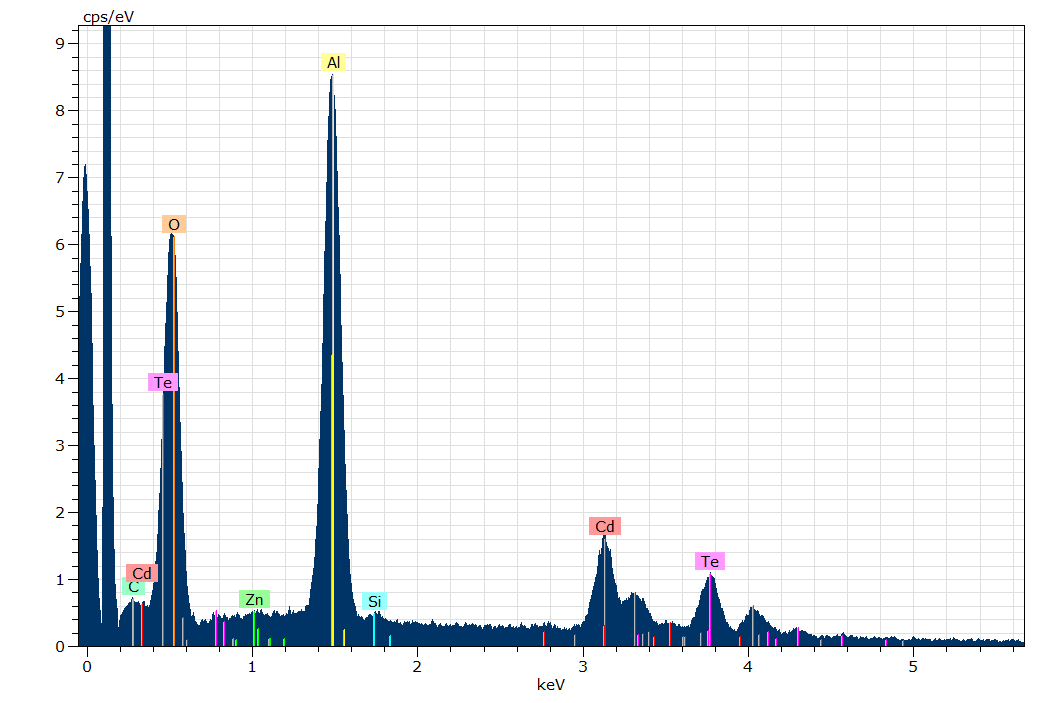
\includegraphics[width=\linewidth]{alumina02_eds.png}
          \end{minipage}
          \begin{minipage}[c]{0.11\linewidth}
            \centering
            \atomicTable[\ce{O}&\SI{46.76}{}][\ce{Al}&\SI{29.78}{}][\ce{C}&\SI{12.14}{}][\ce{Cd}&\SI{5.59}{}][\ce{Te}&\SI{5.05}{}][\ce{Si}&\SI{0.62}{}][\ce{Zn}&\SI{0.04}{}]
          \end{minipage}
    \end{subfigure}%
    \par\bigskip
    \begin{subfigure}[t]{\textwidth}
        \caption{}\label{fig:subBa_polishing-grit_silica}
          \begin{minipage}[c]{0.43\linewidth}
            \centering
            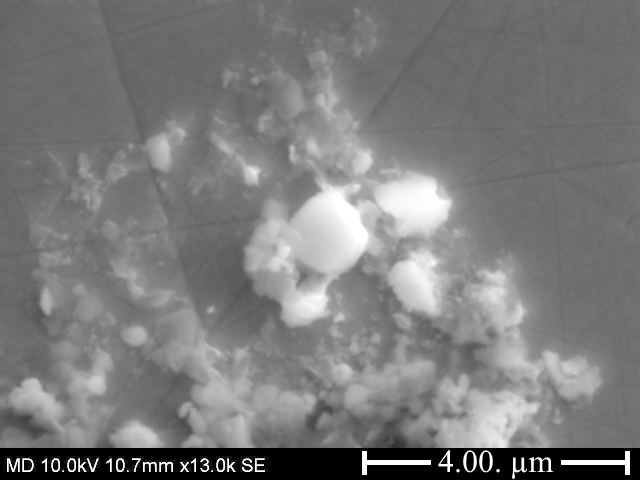
\includegraphics[width=\linewidth]{subB_silica_sem.png}
          \end{minipage}
          \hfill
          \begin{minipage}[c]{0.43\linewidth}
            \centering
            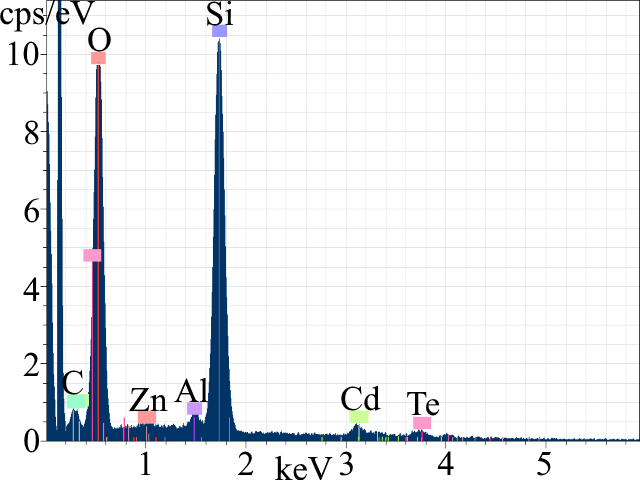
\includegraphics[width=\linewidth]{subB_silica_eds.png}
          \end{minipage}
          \begin{minipage}[c]{0.11\linewidth}
            \centering
            \atomicTable[\ce{O}&\SI{60.33}{}][\ce{Si}&\SI{22.62}{}][\ce{C}&\SI{15.45}{}][\ce{Al}&\SI{0.60}{}][\ce{Te}&\SI{0.47}{}][\ce{Cd}&\SI{0.33}{}][\ce{Zn}&\SI{0.21}{}]
          \end{minipage}
    \end{subfigure}%
    \par\bigskip
    \begin{subfigure}[t]{\textwidth}
        \caption{}\label{fig:SEM_B_particulates_eds}
          \begin{minipage}[c]{0.43\linewidth}
            \centering
            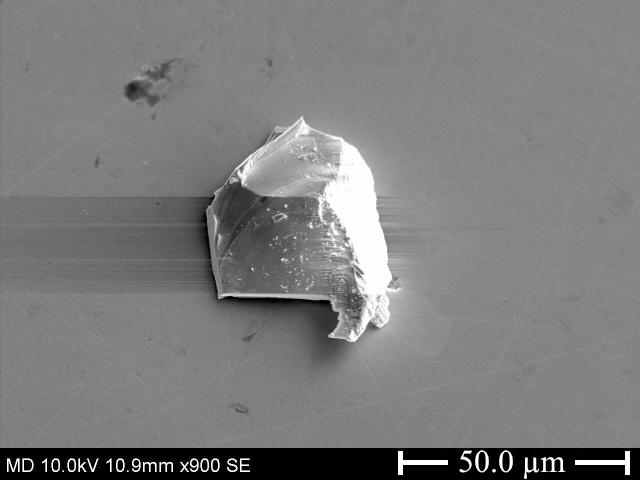
\includegraphics[width=\linewidth]{C-3895-23A_edx1_m006.png}
          \end{minipage}
          \hfill
          \begin{minipage}[c]{0.43\linewidth}
            \centering
            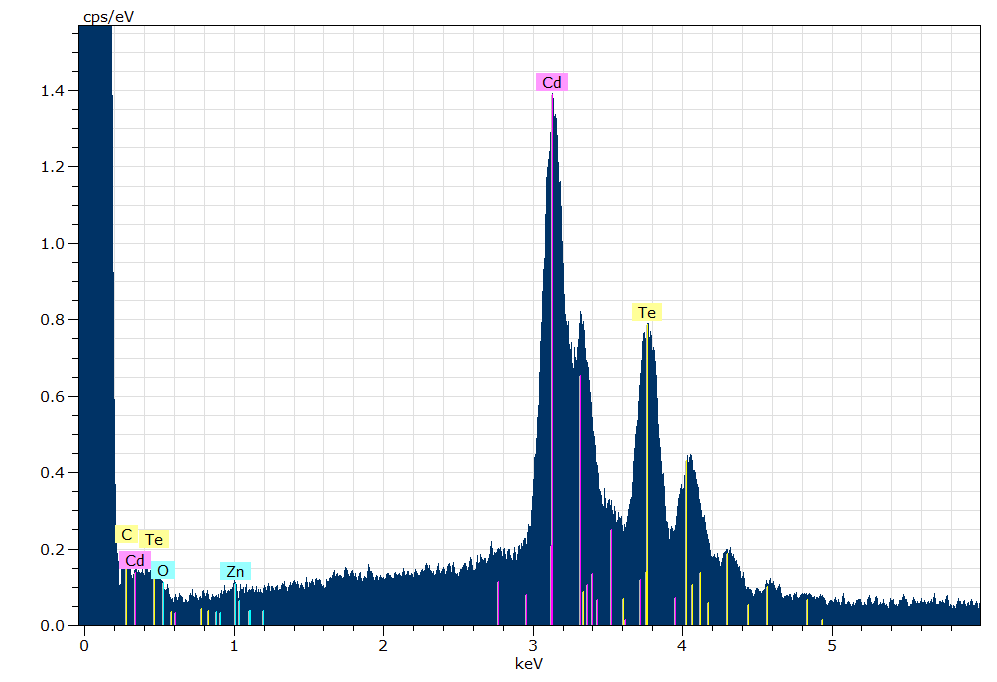
\includegraphics[width=\linewidth]{C-3895-23A_edx1_m006_eds.png}
          \end{minipage}
          \begin{minipage}[c]{0.11\linewidth}
            \centering
            \atomicTable[\ce{Cd}&\SI{46.85}{}][\ce{Te}&\SI{42.07}{}][\ce{C}&\SI{7.90}{}][\ce{Zn}&\SI{1.99}{}][\ce{O}&\SI{1.20}{}]
          \end{minipage}
          %\begin{minipage}[c]{0.49\linewidth}
          %  \centering
          %  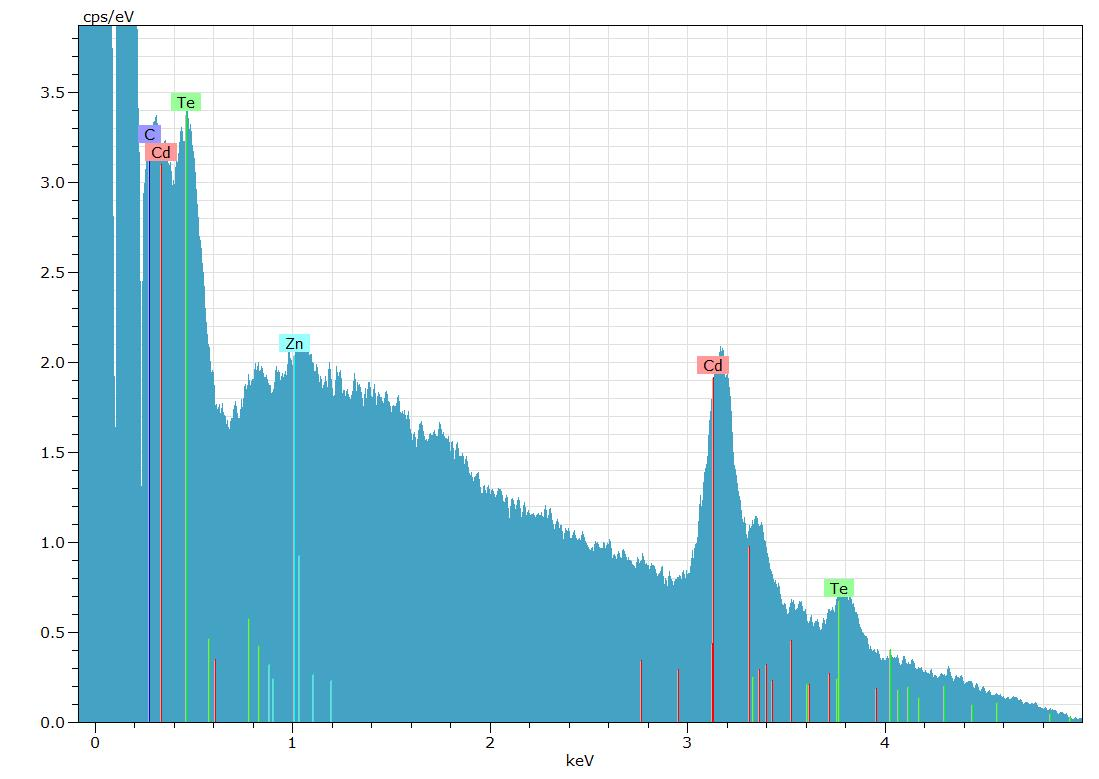
\includegraphics[width=\linewidth]{CdZnTe_eds_substrate.jpg}
          %\end{minipage}
    \end{subfigure}%
    \caption[\Ac{sem} images, \ac{eds} spectra, and \ac{eds} atomic compositions of one void and six different types of particles found on as-received substrate B.]{High resolution \ac{sem} images of one void and six different types of particles found on the as-received substrate B and the corresponding \ac{eds} spectra and atomic compositions: \subref{fig:subBa_polishing-grit_alumina} alumina (\ce{Al2O3}) polishing grit; \subref{fig:subBa_polishing-grit_silica} silica (\ce{SiO2}) polishing grit; \subref{fig:SEM_B_particulates_eds} \ac{czt} paticle; \subref{fig:subBa_particle_carbon} carbon-based particle; \subref{fig:EDS_NaClO} \ce{NaClO}; \subref{fig:subBa_partice_Fe} iron (\ce{Fe}); and \subref{fig:SEM_C389523_void_eds} void.}\label{fig:subBa_sem_w_eds}
\end{figure}
%
\begin{figure}[htbp]
\ContinuedFloat
    \centering
    \begin{subfigure}[t]{\textwidth}
        \caption{}\label{fig:subBa_particle_carbon}
          \begin{minipage}[c]{0.43\linewidth}
            \centering
            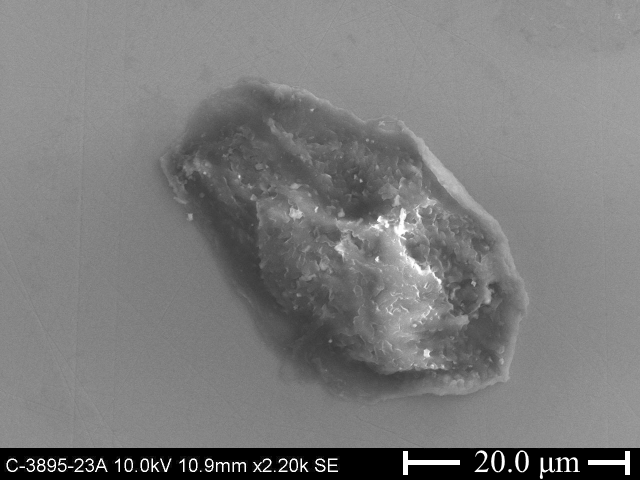
\includegraphics[width=\linewidth]{C-3895-23A_tuning_05.png}%{carbon_eds_sem.jpg} %{C-3895-23_02_m002.jpg}%{C-3895-23A_tuning_05.jpg}
          \end{minipage}
          \hfill
          \begin{minipage}[c]{0.43\linewidth}
            \centering
            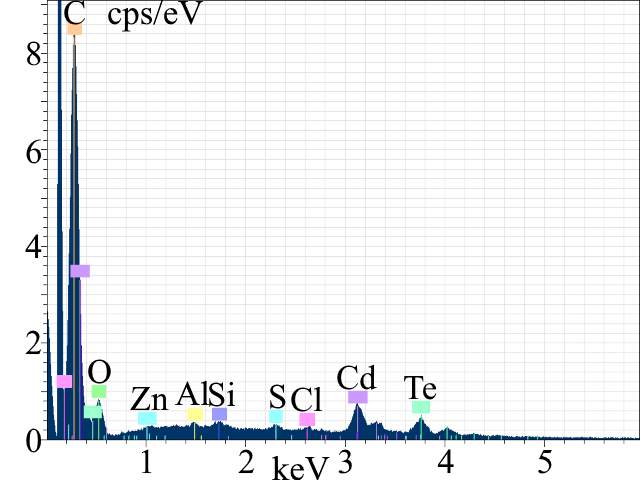
\includegraphics[width=\linewidth]{C-3895-23A_tuning_05_eds.png}
          \end{minipage}
          \begin{minipage}[c]{0.11\linewidth}
            \centering
            \atomicTable[\ce{C}&\SI{86.43}{}][\ce{O}&\SI{7.35}{}][\ce{Cd}&\SI{2.58}{}][\ce{Te}&\SI{2.06}{}][\ce{Si}&\SI{0.55}{}][\ce{S}&\SI{0.36}{}][\ce{Cl}&\SI{0.31}{}][\ce{Zn}&\SI{0.21}{}][\ce{Al}&\SI{0.15}{}]
          \end{minipage}
    \end{subfigure}%
    \par\bigskip
    \begin{subfigure}[t]{\textwidth}
    \caption{}\label{fig:EDS_NaClO}
          \begin{minipage}[c]{0.43\linewidth}
            \centering
            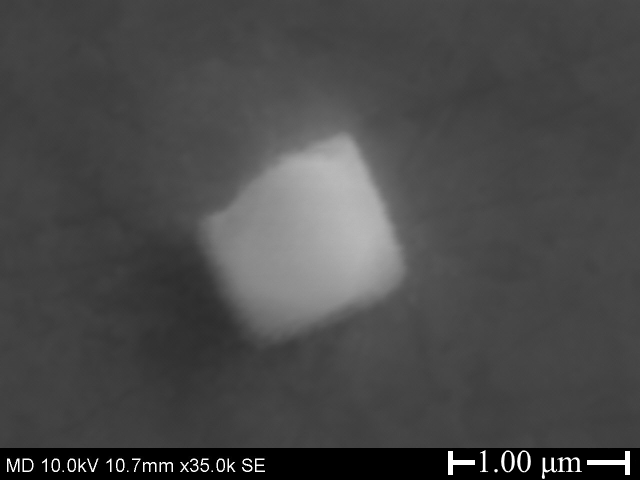
\includegraphics[width=\linewidth]{eds_NaOCl2_C-3895-23A_edx8_m007.png}
          \end{minipage}
          \hfill
          \begin{minipage}[c]{0.43\linewidth}
            \centering
            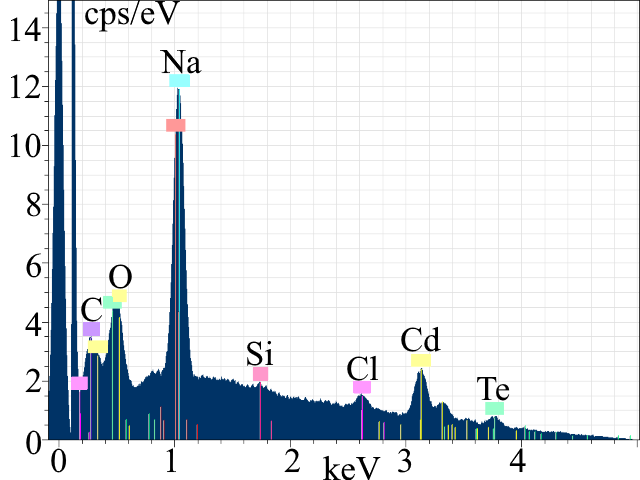
\includegraphics[width=\linewidth]{eds_NaClO2.png}
          \end{minipage}
          \begin{minipage}[c]{0.11\linewidth}
            \centering
            \atomicTable[\ce{Na}&\SI{27.17}{}][\ce{C}&\SI{22.94}{}][\ce{Te}&\SI{20.44}{}][\ce{Cd}&\SI{15.65}{}][\ce{O}&\SI{9.97}{}][\ce{Cl}&\SI{2.45}{}][\ce{Si}&\SI{0.92}{}][\ce{Zn}&\SI{0.47}{}]
          \end{minipage}
    \end{subfigure}%
    \par\bigskip
    \begin{subfigure}[t]{\textwidth}
    \caption{}\label{fig:subBa_partice_Fe}
          \begin{minipage}[c]{0.43\linewidth}
            \centering
            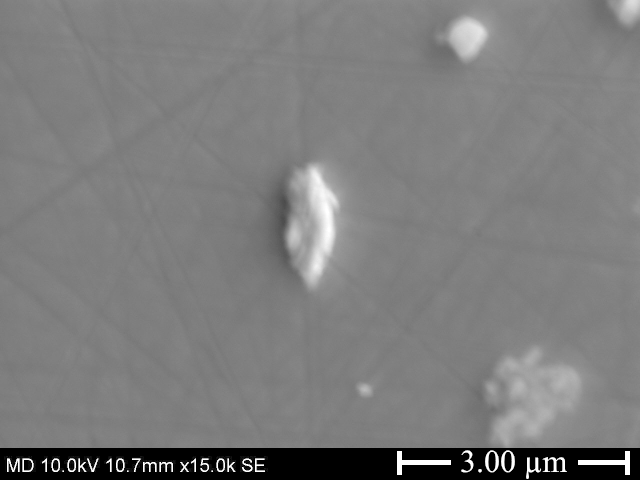
\includegraphics[width=\linewidth]{eds_Fe_C-3895-23A_edx5_m004.png}
          \end{minipage}
          \hfill
          \begin{minipage}[c]{0.43\linewidth}
            \centering
            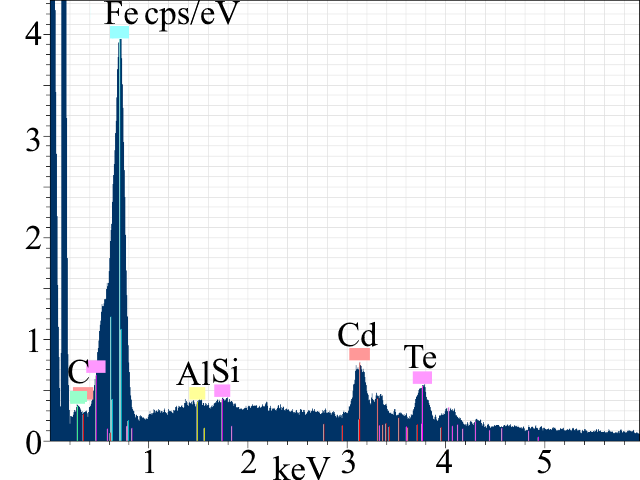
\includegraphics[width=\linewidth]{eds_Fe_C-3895-23A_edx5_m004_eds.png}
          \end{minipage}
          \begin{minipage}[c]{0.11\linewidth}
            \centering
            \atomicTable[\ce{Fe}&\SI{81.79}{}][\ce{C}&\SI{11.21}{}][\ce{Cd}&\SI{3.59}{}][\ce{Te}&\SI{3.04}{}][\ce{Si}&\SI{0.26}{}][\ce{Al}&\SI{0.11}{}]
          \end{minipage}
    \end{subfigure}%
    \captionsetup{list=no}
    \caption{\emph{(continued)}}
\end{figure}
%
\begin{figure}[htbp]
\ContinuedFloat
    \centering
    \begin{subfigure}[t]{\textwidth}
        \caption{}\label{fig:SEM_C389523_void_eds}
          \begin{minipage}[c]{0.43\linewidth}

            \centering
            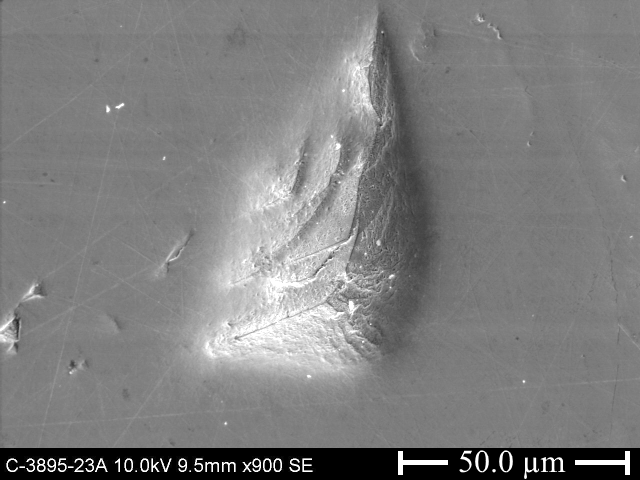
\includegraphics[width=\linewidth]{C-3895-23_09_m001.png}%C-3895-23A_edx3_m001.jpg}
          \end{minipage}
          \hfill
          \begin{minipage}[c]{0.43\linewidth}
            \centering
            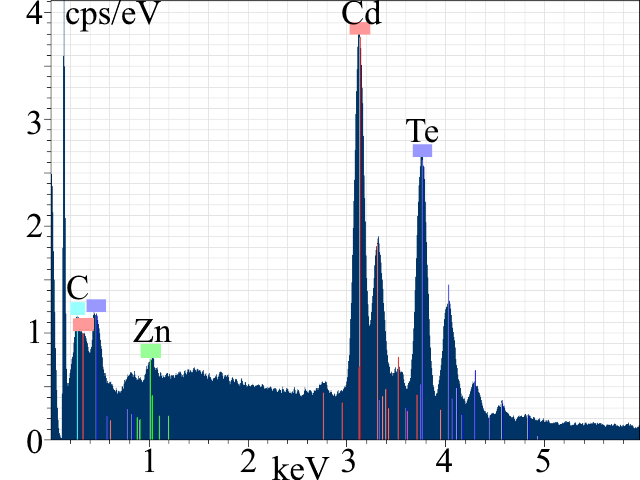
\includegraphics[width=\linewidth]{C-3895-23A_edx3_m001_eds.png}
          \end{minipage}
          \begin{minipage}[c]{0.11\linewidth}
            \centering
            \atomicTable[\ce{Te}&\SI{39.30}{}][\ce{Cd}&\SI{38.80}{}][\ce{C}&\SI{19.94}{}][\ce{Zn}&\SI{1.96}{}]
          \end{minipage}
    \end{subfigure}%
    \captionsetup{list=no}
    \caption{\emph{(continued)}}
\end{figure}

%%=====
\subsubsection{Residual Polishing Grit (alumina and silica)}
Bright particles with varying sizes were observed on the substrate surface, see Fig.~\ref{fig:subBa_polishing-grit_area1}. When looking at one of the accumulations at greater magnification, see Fig.~\ref{fig:subBa_polishing-grit_area2}, it became evident that the large particles were agglomerations of smaller particles. The smaller particles were spherical and had a diameter between \SI{50}{\nano\metre} and \SI{100}{\nano\metre}. The typical width of the particle agglomerations was \SI{0.5}{}-\SI{3}{\micro\metre}. The attraction between the small particles can be explained by electrostatic attractive forces between the particles due to different surface charge \citep{allen2001review}.

\begin{figure}[htbp]
    \centering
        \mySubfigure{0.49\linewidth}{SEM_C-3895-23A_a_m001.png}[fig:subBa_polishing-grit_area1]
        \hfill
        \mySubfigure{0.49\linewidth}{C-3895-23Ab_m003.png}[fig:subBa_polishing-grit_area2]
    \caption[\Ac{sem} images of an accumulaton of polishing grit on substrate B.]{\Ac{sem} images of an accumulation of polishing grit on the as-received substrate B at a magnification of \subref{fig:subBa_polishing-grit_area1} $200\times$ and \subref{fig:subBa_polishing-grit_area2} $15000\times$.}\label{fig:subBa_polishing-grit_area}
\end{figure}

An \ac{eds} spectrum of the particle revealed that the piece was composed of alumina oxide, \ce{Al2O3}, also known as alumina, see Fig.~\ref{fig:subBa_polishing-grit_alumina}. The corresponding \ac{sem} image of residual polishing grit is shown next to the spectrum. The presence of alumina can be explained by the frequent use of alumina as an abrasive in polishing slurries for semiconducting material.

Some of the accumulations were composed of larger particles with a diameter of \SI{600}{\nano\metre} as well as the smaller ones, as seen in Fig.~\ref{fig:subBa_polishing-grit_silica}. An \ac{eds} spectrum of the largest particle revealed that the piece was composed of silicon oxide, \ce{SiO2}, also known as silica. As mentioned earlier, silica is also a frequently used abrasive in polishing slurry.

%%=====
\subsubsection{\Ac{czt}}
%Page 5-6 in eds report 1-10
Bright particles about 10 times as large as the typical polishing grit agglomerations were observed on the substrate surface, see Fig.~\ref{fig:SEM_B_particulates}. The size of the pieces was typically between \SI{50}{\micro\metre} and \SI{100}{\micro\metre}. By comparing the \ac{eds} spectrum of the particle with the spectrum of the substrate surface, see Fig.~\ref{fig:SEM_B_particulates_eds}, it became apparent that the particles had the same composition as the surrounding substrate. This indicates that the pieces could be debris from the polishing or cutting of the substrate.

\begin{figure}[htbp]
    \centering
          \begin{minipage}[c]{0.49\linewidth}
            \centering
            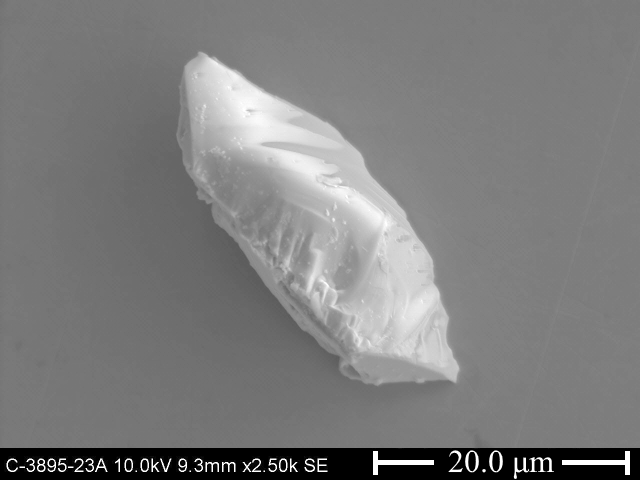
\includegraphics[width=\linewidth]{C-3895-23_03.png}
          \end{minipage}
          \hfill
          \begin{minipage}[c]{0.49\linewidth}
            \centering
            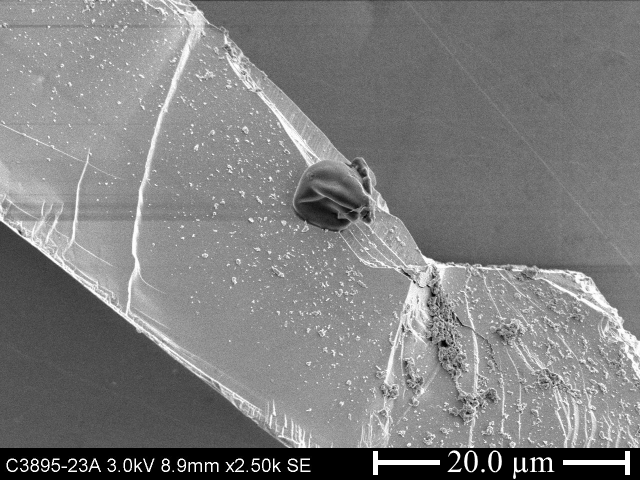
\includegraphics[width=\linewidth]{C-3895-23Af2_m002.png}
          \end{minipage}
        \caption[\Ac{sem} images of \ac{czt} particles on as-revceived substrate B.]{\Ac{sem} images of \ac{czt} particles on the as-revceived substrate B.}\label{fig:SEM_B_particulates}  
\end{figure}


%%=====
\subsubsection{Carbon-based particle}
Dark particles, which typically had a size between \SIrange{20}{30}{\micro\metre}, were observed on the substrate surface, as seen in Fig.~\ref{fig:subBa_particle_carbon}. The \ac{eds} spectrum of this particle showed a high intensity from the carbon signal. The particles could be residue from mounting wax, which was used to hold the substrate while it was being cut and polished. Some small peaks of silicon and aluminium were observed as well, but they probably stemmed from the residual polishing grit that can be seen in on the surface of the carbon-based particle.
%Page 8+12 in eds report 1-10

%%=====
\subsubsection{\ce{NaClO}}
An area with lots of circular particles with a diameter between \SI{100}{\nano\metre}--\SI{1}{\micro\metre} was observed near one of the edges of substrate B, see Fig.~\ref{fig:eds_NaOCl_overview}. The area was separated from the rest of the substrate by a dark borderline. An \ac{eds} spectrum of one particle with a diameter of \SI{1}{\micro\metre}, see Fig.~\ref{fig:EDS_NaClO}, reveals that the particle consists of \ce{Na}, \ce{Cl}, and \ce{O}. The particles could be \ce{NaClO} which typically is used after polishing as a standard cleaner to remove polishing slurry particles \citep{benson2015as-received}. The dark borderline was not possible to get quantified with \ac{eds}, but it could be a residue of the cleaning solution.

\begin{figure}[htbp]
    \centering
    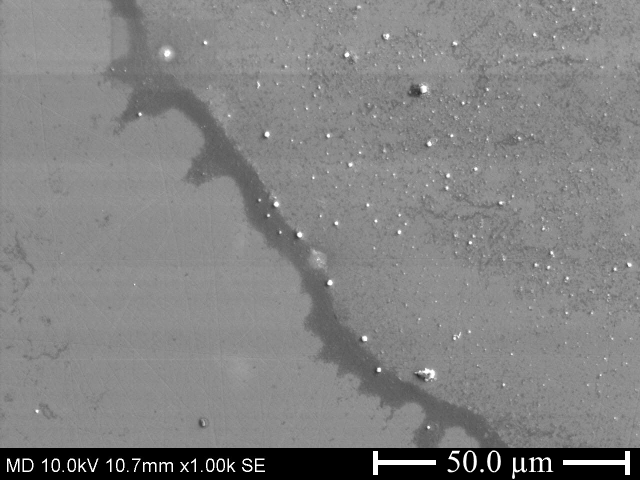
\includegraphics[width=0.48\linewidth]{eds_NaOCl_overview_C-3895-23A_edx8_m008.png}
    \caption[\Ac{sem} image of \ce{NaClO} particles on substrate B.]{\Ac{sem} image of \ce{NaClO} particles on substrate B.}
    \label{fig:eds_NaOCl_overview}
\end{figure}

%%=====
\subsection{Iron Particle}
A small particle that was \SI{1.5}{\micro\metre} long and \SI{0.6}{\micro\metre} wide can be seen in Fig.~\ref{fig:subBa_partice_Fe} with its corresponding \ac{eds} spectrum. The \ac{eds} spectrum of the particle revealed that the particle consisted mainly of \ce{Fe}. Iron is a potential contaminate in polishing grit slurry, but it could also originate in cross-contamination from the polishing of other semiconductors, i.e. \ce{InP} \citep{benson2015as-received}.

%%=====
\subsubsection{Voids}
%Page b1 in eds report 1-10
Irregular shaped voids were observed all over the surface of substrate B, see Fig.~\ref{fig:SEM_C389523_voids}. The width of the voids tended to be between \SIrange{5}{100}{\micro\metre} and \ac{afm} measurements gave that the voids were between \SIrange{1.3}{2.5}{\micro\metre} deep, see Fig.~\ref{fig:subBa_afm_voids}. \Ac{eds} detected \ce{Cd_{0.96}Zn_{0.04}Te} both on the inside edges of the voids and around the voids, see Fig.~\ref{fig:SEM_C389523_void_eds}. This revealed that the voids had the same composition as the substrate surface.

\begin{figure}[htbp]
    \centering
    \begin{subfigure}[t]{\textwidth}
    \caption{}\label{fig:subBa_voids}
          \begin{minipage}[c]{0.49\linewidth}
            \centering
            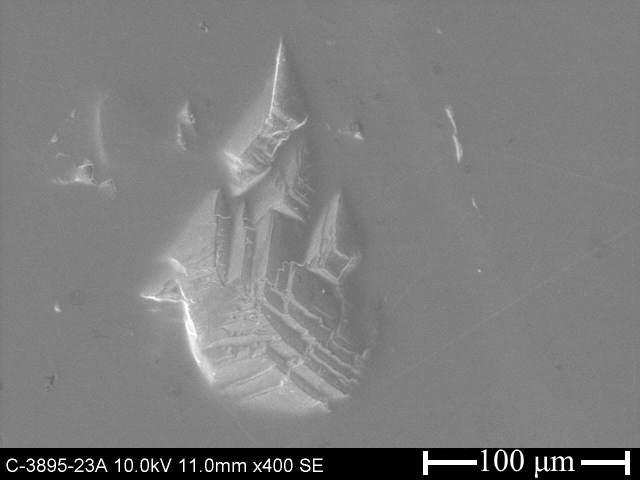
\includegraphics[width=\linewidth]{C-3895-23A_tuning_04.png}
          \end{minipage}
          \hfill
          \begin{minipage}[c]{0.49\linewidth}
            \centering
            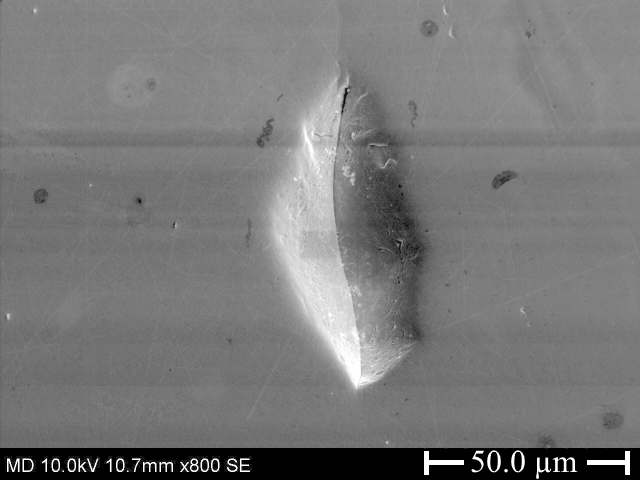
\includegraphics[width=\linewidth]{C-3895-23A_edx3_m002.png}
          \end{minipage}
    \end{subfigure}%
    \par\bigskip
    %\mySubfigure[SEM.]{0.44\linewidth}{C-3895-23A_edx7_m002.jpg}
    %\mySubfigure[SEM.]{0.44\linewidth}{C-3895-23A_edx7_m003.jpg}
    \begin{subfigure}[t]{\textwidth}
    \caption{}\label{fig:subBa_microvoids}
          \begin{minipage}[c]{0.49\linewidth}
            \centering
            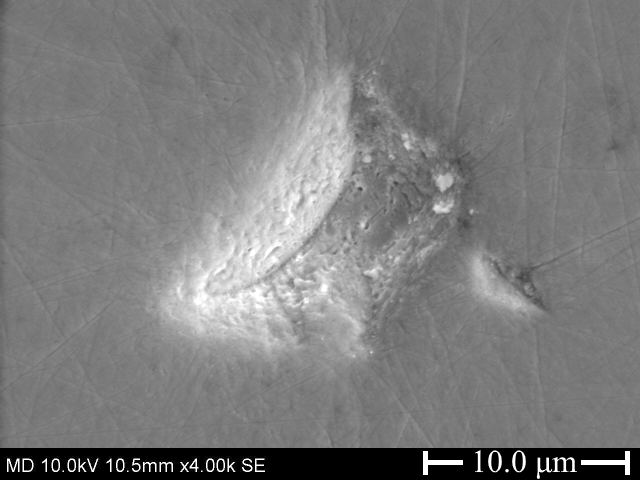
\includegraphics[width=\linewidth]{C-3895-23A_edx7_m004.png}
          \end{minipage}
          \hfill
          \begin{minipage}[c]{0.49\linewidth}
            \centering
            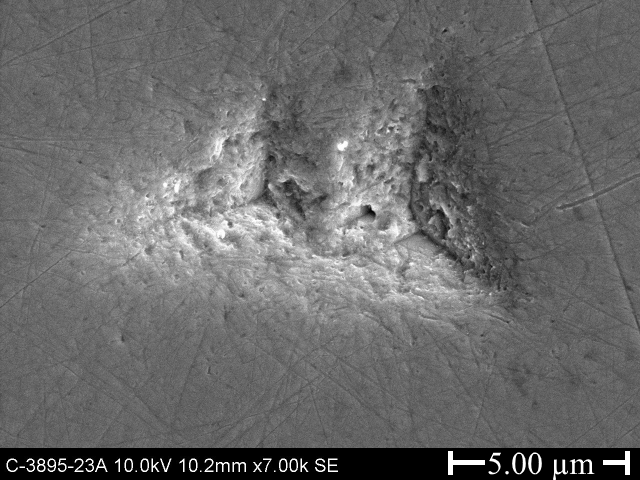
\includegraphics[width=\linewidth]{C-3895-23A_K01_detail.png}
          \end{minipage}
    \end{subfigure}%
    \caption[\Ac{sem} images of voids on substrate B.]{\Ac{sem} images of \subref{fig:subBa_voids} large voids \SI{>10}{\micro\metre} and \subref{fig:subBa_microvoids} small voids \SI{<10}{\micro\metre} on the as-received substrate B.}
    \label{fig:SEM_C389523_voids}
\end{figure}

\begin{figure}
    \centering
    \begin{subfigure}[c]{0.032\linewidth}
        \label{fig:subBa_afm_voids_scale}\captionsetup{list=no}
        
\includegraphics[width=\linewidth]{subBa_afm_voids_scale.png}
    \end{subfigure}
    \hfill
    \mySubfigure{0.46\linewidth}{subBa_afm_void_170201Topography013.png}[fig:subBa_afm_void]
    \hfill
    \mySubfigure{0.46\linewidth}{subBa_afm_microvoid_170201Topography005.png}[fig:subBa_afm_microvoid]
    \caption[\Ac{afm} measurements of voids on as-received substrate B.]{\Ac{afm} measurements of \subref{fig:subBa_afm_void} a \SI{40}{\micro\metre} wide void and \subref{fig:subBa_afm_microvoid} a \SI{7}{\micro\metre} wide void on the as-received substrate B displayed as images of $\SI{50}{\micro\metre}\times\SI{50}{\micro\metre}$ and $\SI{10}{\micro\metre}\times\SI{10}{\micro\metre}$ areas respectively.}
    \label{fig:subBa_afm_voids}
\end{figure}

Some of the smaller voids have a threefold symmetry, as seen in Fig.~\ref{fig:subBa_microvoids}. The larger voids \SI{>10}{\micro\metre} tended to have multiple angular features, as seen in Fig.~\ref{fig:subBa_voids}. \citet{reddy2013cross} speculate that these voids originally was occupied by a tellurium precipitate that was knocked loose during surface preparation, i.e. substrate polishing in this case, leaving a void on the surface. This theory is supported by the fact that tellurium precipitates often are crystalline and could be the source of the angular features of the voids \citep{wang2008observation}.

\begin{figure}[htbp]
    \centering
        \mySubfigure{0.403\linewidth}{subBa_densityData_voids.png}[fig:subBa_densityData_void_map]
        \hfill
        \mySubfigure{0.577\linewidth}{C-3895-23A_A01_x060.png}[fig:subBa_densityData_void_sem]
    \caption[Map of the void density on the as-received substrate B.]{\subref{fig:subBa_densityData_void_map} A map of the void density at 36 different locations on the as-received $\SI{30}{\milli\metre}\times\SI{30}{\milli\metre}$ substrate B. The density measurements were obtained by counting the number of voids in \ac{sem} images covering $\SI{254}{\micro\metre}\times\SI{178}{\micro\metre}$ areas. In total, \SI{0.2}{\percent} of the substrate surface was measured. The void density was observed to vary between \SIrange{2e+03}{2e+4}{\centi\metre^{-2}}. \subref{fig:subBa_densityData_void_sem} An image from the upper right corner of the grid where the void density is highest.}
    \label{fig:subBa_densityData_voids}
\end{figure}

The void density was found to be between \SIrange{2e+03}{2e+4}{\centi\metre^{-2}}. The mean void density was \SI{7e+03}{\centi\metre^{-2}} with a standard deviation of \SI{5e+03}{\centi\metre^{-2}}. A graphical representation of the void density at different locations on substrate B can be seen in Fig.~\ref{fig:subBa_densityData_voids}.

\begin{comment}
The void density was found to be between \SI{1e+02}{\centi\metre^{-2}} and \SI{2e+3}{\centi\metre^{-2}}. The mean void density was \SI{4e+02}{\centi\metre^{-2}} with a standard deviation of \SI{3e+02}{\centi\metre^{-2}}. A graphical representation of the void density at different locations on substrate B can be seen in Fig.~\ref{fig:subBa_densityData_largevoid}.

\begin{figure}[htbp]
    \centering
        \mySubfigure{0.403\linewidth}{subBa_densityData_largevoids.png}[fig:subBa_densityData_largevoid_map]
        \hfill
        \mySubfigure{0.577\linewidth}{C-3895-23A_A01_x060.png}[fig:subBa_densityData_largevoid_sem]
    \caption[Map of the large void density on the as-received substrate B.]{\subref{fig:subBa_densityData_void_map} A map of the large void density at 36 different locations on the as-received $\SI{30}{\milli\metre}\times\SI{30}{\milli\metre}$ substrate B. The large void density was observed to vary between \SI{1e+02}{\centi\metre^{-2}} and \SI{2e+3}{\centi\metre^{-2}}. \subref{fig:subBa_densityData_void_sem} An image from the upper right corner of the grid where the large void density is highest.}
    \label{fig:subBa_densityData_void}
\end{figure}

The microvoid density was found to be between \SI{2e+03}{\centi\metre^{-2}} and \SI{2e+4}{\centi\metre^{-2}}. The mean microvoid density was \SI{6e+03}{\centi\metre^{-2}} with a standard deviation of \SI{5e+03}{\centi\metre^{-2}}. A graphical representation of the microvoid density at different locations on substrate B can be seen in Fig.~\ref{fig:subBa_densityData_microvoid}.
%Voids: Minimum = 1.28e+02. Maximum = 1.91e+03. Mean = 4.20e+02. Standard deviation = 3.26e+02.
%Microvoids: Minimum = 2.21e+03. Maximum = 2.21e+04. Mean = 6.09e+03. Standard deviation = 5.06e+03

\begin{figure}[htbp]
    \centering
        \mySubfigure{0.403\linewidth}{subBa_densityData_microvoids.png}[fig:subBa_densityData_microvoid_map]
        \hfill
        \mySubfigure{0.577\linewidth}{C-3895-23A_A11_x500.png}[fig:subBa_densityData_microvoid_sem]
    \caption[Map of the microvoid density on the as-received substrate B.]{\subref{fig:subBa_densityData_microvoid_map} A map of the microvoid density at 36 different locations on the as-received $\SI{30}{\milli\metre}\times\SI{30}{\milli\metre}$ substrate B. The microvoid density was observed to vary between \SI{2e+03}{\centi\metre^{-2}} and \SI{2e+4}{\centi\metre^{-2}}. \subref{fig:subBa_densityData_microvoid_sem} An image from the upper right corner of the grid where the microvoid density is highest.}
    \label{fig:subBa_densityData_microvoid}
\end{figure}
\end{comment}

%%=====
\subsection{Circular stains}
Four typical stains that were observed on the substrate surface with \ac{sem} is shown in Fig.~\ref{fig:subB_stains}. One type of stain had a bright background with a darker centre in one part of the stain, as seen in Fig.~\ref{fig:EDX_C-3895-23Ad_m001}--\oldsubref{fig:EDX_C-3895-23A_edx1_m005}. The size of the bright stains varies from \SI{30}{\micro\metre} to \SI{150}{\micro\metre}. The density of this type of stain was estimated from the \ac{sem} grid map to be \SI{2e2}{\centi\metre^{-2}}. These stains could be residue from the evaporation of a droplet on the surface, with the centre consisting of the impurities that were carried by the surface tension of the droplet. %The bright background could be a thin layer of ...

\begin{figure}[htbp]
    \centering
    \mySubfigure{0.48\linewidth}{C-3895-23A_edx1_m001.png}[fig:EDX_C-3895-23Ad_m001]
    \mySubfigure{0.48\linewidth}{C-3895-23A_edx1_m005.png}[fig:EDX_C-3895-23A_edx1_m005]
    \par\bigskip
    \mySubfigure{0.48\linewidth}{C-3895-23A_edx1_m003.png}[fig:EDX_C-3895-23A_edx1_m003]
    \mySubfigure{0.48\linewidth}{C-3895-23A_edx1_m016.png}[fig:EDX_C-3895-23A_edx1_m016]
    \caption[\Ac{sem} images of stains on substrate B.]{\Ac{sem} images of \subref{fig:EDX_C-3895-23Ad_m001}--\subref{fig:EDX_C-3895-23A_edx1_m005} bright and \subref{fig:EDX_C-3895-23A_edx1_m003}--\subref{fig:EDX_C-3895-23A_edx1_m016} dark stains on substrate B.}
    \label{fig:subB_stains}
\end{figure}

A second type of stain, as seen Fig.~\ref{fig:EDX_C-3895-23A_edx1_m003}, appeared dark in the \ac{sem} images and had sizes ranging between \SIrange{8}{15}{\micro\metre}. The density of these stains was estimated from the \ac{sem} grid map to be \SI{1e3}{\centi\metre^{-2}}. The third type of stain appeared as a dark shadow on the substrate surface when observed in \ac{sem}, see Fig.~\ref{fig:EDX_C-3895-23A_edx1_m016}. The typical size of these stains were \SIrange{10}{50}{\micro\metre} and the density of these stains was estimated to be \SI{1e4}{\centi\metre^{-2}}. The observed stains do not contribute any additional signal to the \ac{eds} spectrum due to their thin layer on the surface. Hence, it has not been possible to identify what the composition of the stains were. 
%Page 11 in eds report 1-10

%%=========================================
%\section{AFM Study of As-Received Substrate B}
\subsection{Surface Scratches and Roughness}
The surface of substrate B had been subjected to a coarse polish, and scratches stemming from the polishing could be seen on the surface. The scratches were typically between \SIrange{10}{100}{\nano\metre} wide, as seen in Fig.~\ref{fig:C-3895-23Ad_m002}. Some large scratches were located close to the edges and were as wide as \SI{1}{\micro\metre}, as seen in Fig.~\ref{fig:C-3895-23A_J08_detail}. The latter were not as evenly distributed as the polishing scratches, and they are typical of handling tools, i.e. the teflon tweezers. \todo{Ta vekk disse (fra bilde også) siden det er laget av oss.} surface scratches on substrate B are most likely deeper than those on substrate A since they are visible on the dark field images of substrate B. Substrate B needs a fine polishing before growth to get rid of the scratches.
\begin{figure}[htbp]
    \centering
    \mySubfigure{0.48\linewidth}{C-3895-23Ad_m002.png}[fig:C-3895-23Ad_m002]
    \mySubfigure{0.48\linewidth}{C-3895-23A_J08_detail.png}[fig:C-3895-23A_J08_detail]
    \caption[\Ac{sem} images of scratches on substrate B.]{\Ac{sem} images of \subref{fig:C-3895-23Ad_m002} polishing scratches and \subref{fig:C-3895-23A_J08_detail} deep scratches on substrate B.}
    \label{fig:SEM_C389523_scratches}
\end{figure}

Complementary \ac{afm} images are shown in Fig.~\ref{fig:subBa_afm} where $\SI{5}{\micro\metre}\times\SI{5}{\micro\metre}$ areas were measured at three different locations on the substrate surface: near the centre, upper edge, and upper left corner. The \ac{rms} roughness of substrate B was \SI{\sim 3.7}{\nano\metre} at the centre and \SI{\sim 4.8}{\nano\metre} around the edges and corners, which is a factor \SIrange{12}{16}{} larger than the \ac{rms} roughness measured on substrate A. This indicates that the substrate has large scratches and is inferior to substrate A. With too large \ac{rms} roughness, the surface starts looking 3-dimensional instead of 2-dimensional, resulting in poorer film growth (R. Haakenaasen, personal communication, May 29, 2017). The \ac{czt} substrate surfaces are easily damaged by surface scratches caused by mechanical lapping \citep{egan2009scanning}. The final polishing step performed by the vendor had left scratches on the surface, as can be observed in all the \ac{afm} images. The largest polishing scratches on substrate B were \SI{0.3}{\micro\metre} wide and \SI{15}{\nano\metre} deep.

\begin{figure}[htbp]
    \centering
    \begin{subfigure}[c]{0.032\linewidth}
        \label{fig:subBa_afm_scale}\captionsetup{list=no}
        
\includegraphics[width=\linewidth]{subBa_afm_scale.png}
    \end{subfigure}
    \hfill
    \mySubfigure{0.3\linewidth}{subBa_afm_centre.png}[fig:subBa_afm_centre]
    \hfill
    \mySubfigure{0.3\linewidth}{subBa_afm_leftedge.png}[fig:subBa_afm_edge]
    \hfill
    \mySubfigure{0.3\linewidth}{subBa_afm_upperleftcorner.png}[fig:subBa_afm_corner]
    \caption[\Ac{afm} of as-received substrate B.]{\Ac{afm} measurements of the as-received substrate B. Images of $\SI{5}{\micro\metre}\times\SI{5}{\micro\metre}$ areas are taken at three different locations on the substrate surface: \subref{fig:subBa_afm_centre} near the centre, \ac{rms} roughness \SI{3,7}{\nano\metre}; \subref{fig:subBa_afm_edge} near the left edge, \ac{rms} roughness \SI{4,8}{\nano\metre}; and \subref{fig:subBa_afm_corner} near the upper left corner, \ac{rms} roughness \SI{4,8}{\nano\metre}. The bright line near the top of the image is due to the tip losing track of the surface.}\label{fig:subBa_afm}
\end{figure} % AFM, substrate B, as-received.

%%=========================================
%\section{Near-IR of As-Received Substrate B}

%%=========================================
\subsection{Impurity Analysis -- EDS}

\Ac{eds} impurity analysis was performed on the as-received substrate B. Three locations on the surface -- the centre, the edge, and the corner -- were analysed. The results of this analysis can be seen in Table~\ref{tab:subBa_eds_analysis}. The only elements found above the \ac{eds} detection limit, in addition to \ce{Cd}, \ce{Zn}, and \ce{Te}, were \ce{Al}, \ce{Si}, \ce{C}, and \ce{O}. The relative concentrations of \ce{Cd}, \ce{Zn}, and \ce{Te} had an error of less than one percentage point from the expected value of \SI{48}{\atomic\percent} cadmium, \SI{2}{\atomic\percent} zinc, and \SI{50}{\atomic\percent} tellurium. The atomic concentration of aluminium and silicon near the centre of the substrate is slightly lower compared to the concentrations near the edge and corner\todo{}. \todo{Mer Si enn på A?}

\begin{table}[htbp]
    \centering
    \caption[\Ac{eds} impurity analysis of the as-received substrate B.]{Results of the \ac{eds} impurity analysis at three different locations on the $\SI{30}{\milli\metre}\times\SI{30}{\milli\metre}$ as-received (111)B \ac{czt} substrate B (atomic concentration \%). The X-ray signal was acquired from $\SI{1270}{\micro\metre}\times\SI{890}{\micro\metre}$ areas near the centre, upper edge, and upper left corner.}\label{tab:subBa_eds_analysis}
    \begin{tabu} to 1.0\textwidth { X[1.85,r] X[1.125,c] X[1.125,c] X[1.125,c] X[1.125,c] X[1.125,c] X[1.125,c] X[1.125,c] }
    \hline
         & \textbf{\ce{Te}} (at.\%) & \textbf{\ce{Cd}} (at.\%) & \textbf{\ce{Zn}} (at.\%) & \textbf{\ce{Al} } (at.\%) & \textbf{\ce{Si}} (at.\%) & \textbf{\ce{C}} (at.\%) & \textbf{\ce{O}} (at.\%) \\ % \textbf{$X$} (\SI{}{\milli\metre}) &  \textbf{$Y$} (\SI{}{\milli\metre})
        \hline
        Near centre & \SI{45.88}{} & \SI{45.35}{} & \SI{2.13}{} & \SI{0.18}{} & \SI{0.47}{} & \SI{4.59}{} & \SI{1.40}{}  \\ %\SI{15.1}{} & \SI{15.1}{}
        Near edge & \SI{45.84}{} & \SI{45.39}{} & \SI{2.28}{} & \SI{0.21}{} & \SI{0.51}{} & \SI{4.59}{} & \SI{1.18}{}   \\ % \SI{15.1}{} & \SI{29.0}{}
        Near corner & \SI{45.86}{} & \SI{45.45}{} & \SI{2.28}{} & \SI{0.36}{} & \SI{0.49}{} & \SI{4.23}{} & \SI{1.33}{}  \\ %\SI{1.0}{}  & \SI{29.0}{}
         \hline
    \end{tabu}
\end{table}
%%========================================
% FTIR transmission spectra.
\subsection{IR Characterisation}

\Ac{ftir} transmission spectra were recorded from an $11\times11$ grid on the as-received substrate B2. The grid points were placed \SI{2.0}{\milli\metre} from the edge and had \SI{2.6}{\milli\metre} between nearest neighbours. The spectra measured in the upper half of substrate B2 had the same characteristics as substrate A, and hence, had the same properties regarding precipitates and carrier concentration as substrate A \citep{yujie2004infrared}. Some of the spectra measured in the lower half of the substrate deviated by having a downward slope for lower wavenumbers, see Fig.~\ref{fig:subB2a_ftir_spectra}. These spectra had a value of $T_{5000}$ \SI{<60}{\percent} and $T_{1000}$ \SI{\ll 60}{\percent}. According to \citet{yujie2004infrared}, \ac{czt} substrates with these parameters have a higher free carrier concentration, on the order of  \SI{e17}{\centi\metre^{-2}}, and a lower resistivity than the other spectra. The area of low-transmission form a semicircle in the lower part of substrate B2, as seen in Fig.~\ref{fig:subB2a_ftir_map_500cm-1}. %\todo{Why resisitivity?} % and resistivity of the order \SI{e2}{\ohm\centi\metre} Aa: e6 ohm centi metre

\begin{figure}[htbp]
    \centering
    \mySubfigure{0.60175438596\linewidth}{subB2a_121_ftir_spectra.png}[fig:subB2a_ftir_spectra]
    \hfill
    \mySubfigure{0.37824561403\linewidth}{subB2a_121_ftir_transmission_at_k500cm-1.png}[fig:subB2a_ftir_map_500cm-1]
    \caption[\Ac{ftir} measurements of the as-received substrate B2.]{\Ac{ftir} measurements recorded from a $11\times11$ grid on the as-received $\SI{30}{\milli\metre}\times\SI{30}{\milli\metre}$ (111)B-oriented substrate B2: \subref{fig:subB2a_ftir_spectra} Transmission spectra; \subref{fig:subB2a_ftir_map_500cm-1} transmission map at wavenumber $k=\SI{500}{\centi\metre^{-1}}$ showing the transmittance $T$ in percentage of incoming light at each grid point. The spikes near $k=\SI{4500}{\centi\metre^{-1}}$ and $k=\SI{5000}{\centi\metre^{-1}}$ were artefacts of the \ac{ftir} instrument.}
\end{figure}

Surprisingly, the low-transmission semicircle was visible as a brighter area in the \ac{sem} images, see Fig.~\ref{fig:subB2b_sem_low_transmission}. The semicircle started \SI{4.11}{\milli\metre} from the left edge, went around up to \SI{13.11}{\milli\metre} before it went down, and ended \SI{1.89}{\milli\metre} from the right edge. The major influence on \ac{se} generation is the topography of the surface, and generally, edges and other pointy parts that are facing the detector produce more \acp{se}, and hence, these parts look brighter than the rest of the image \citep{goldstein2012scanning}. This was not the case for the brighter area because \ac{afm} measurements affirmed that the surface was as uniform and smooth as the surrounding substrate. Also, the average atomic number influences the contrast, but \ac{eds} spectra confirmed that the low-transmission area and the surrounding substrate had the same composition.

\begin{figure}[htbp]
    \centering
    \mySubfigure{0.49\linewidth}{subB2b_sem_04_m007.png}[fig:subB2b_sem_low_transmission_left]
    \hfill
    \mySubfigure{0.49\linewidth}{subB2b_sem_04_m005.png}[fig:subB2b_sem_low_transmission_right]
    %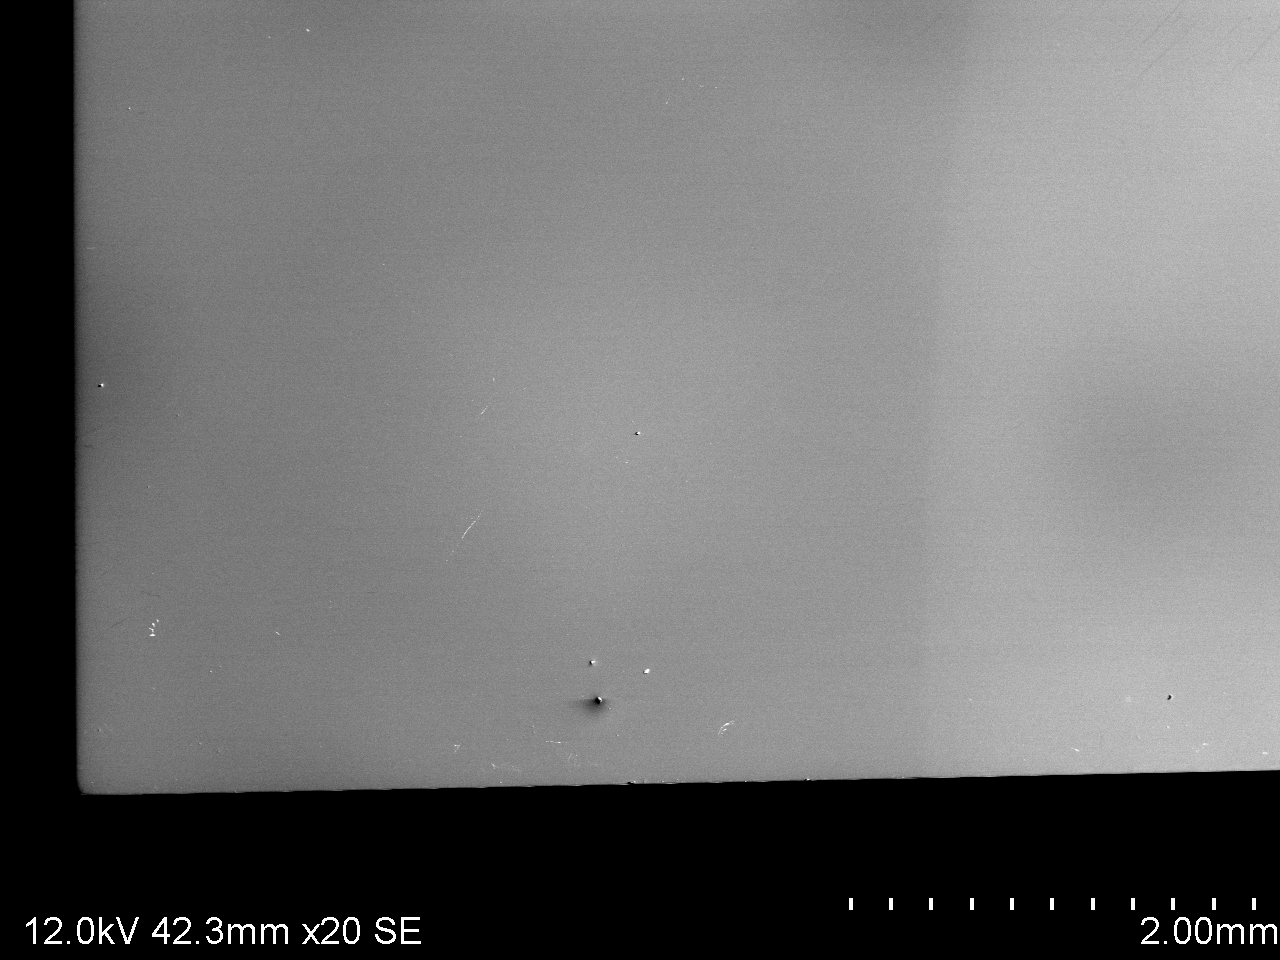
\includegraphics[width=1.0\linewidth]{subB2b_sem_05_m002.png}\caption{Left edge}
    %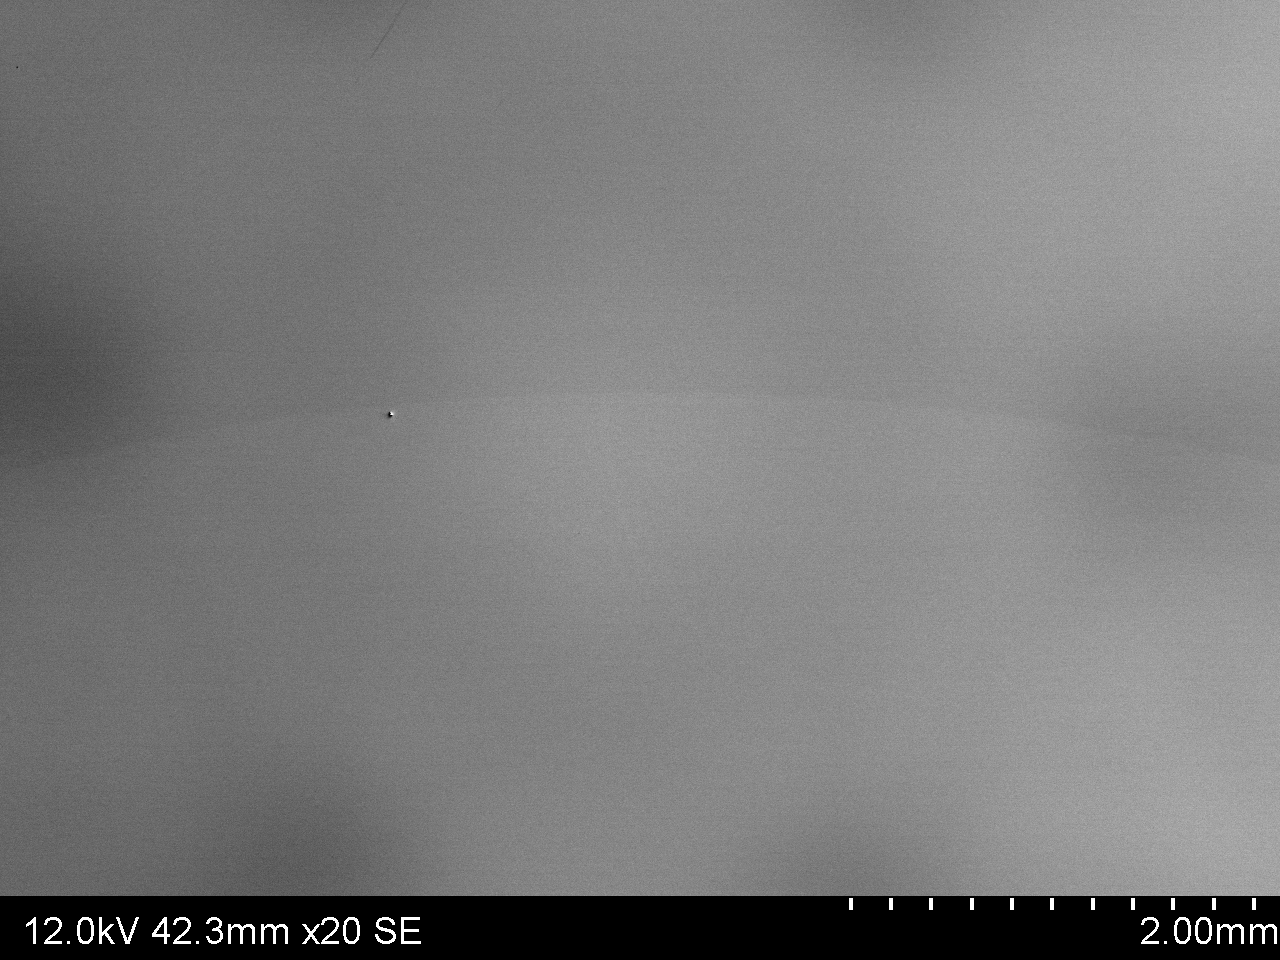
\includegraphics[width=1.0\linewidth]{subB2b_sem_05_m005.png}\caption{Upper edge}
    %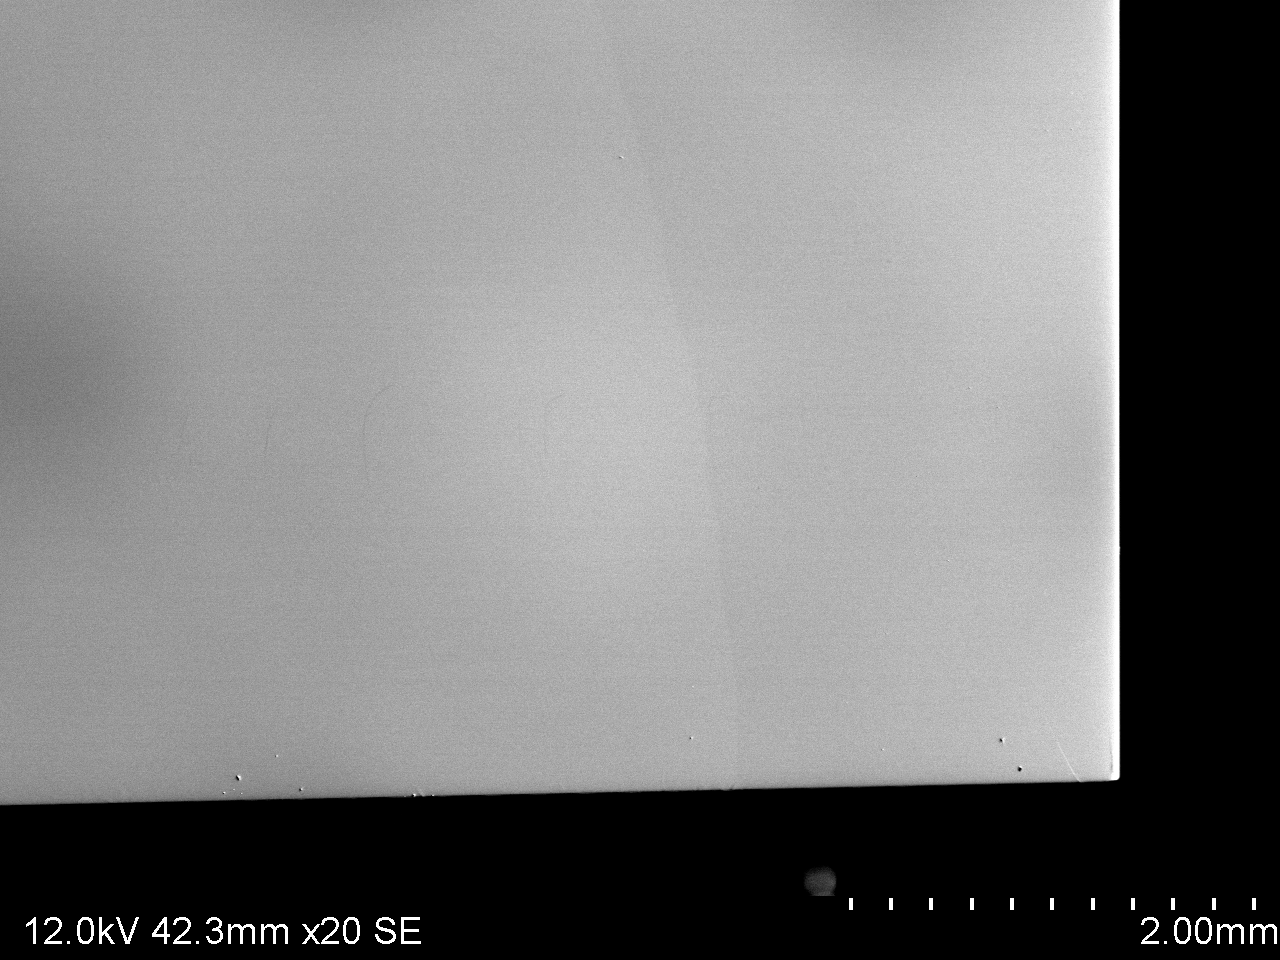
\includegraphics[width=1.0\linewidth]{subB2b_sem_05_m003.png}\caption{Right edge}
    \caption[\Ac{sem} image of the semicircle with low \ac{ir} transmission on substrate B2.]{\Ac{sem} image of the \subref{fig:subB2b_sem_low_transmission_left} left and \subref{fig:subB2b_sem_low_transmission_right} right edge of the semicircle with low \ac{ir} transmission in the lower part of substrate B2. The semicircle appears brighter than the rest of the substrate surface.}\label{fig:subB2b_sem_low_transmission}
\end{figure}

It could be different crystal orientation that caused the contrast in the \ac{sem} images in Fig.~\ref{fig:subB2b_sem_low_transmission}. \Ac{lpe} growth is particularly sensitive for the crystal orientation of the substrate (E. Selvig, personal communication, May 24, 2017). However, the films which were grown on this kind of low-transmission areas were not affected, and hence, it had likely not a different crystal orientation. 

\citet{sealy2000mechanism} showed that p-type semiconductors in general appeared brighter and that n-type in general appeared darker than undoped material in \ac{sem}. The best contrast was achieved when using low voltage because then the number of electrons that escaped the sample had a stronger dependency on the doping in the sample. Doping contrast agreed with the expected concentration of free carriers for the sloping spectra, which was observed at the low-transmission semicircle.


\todo{Randi: Could it be an absorbing layer of some sort? Further work: turn down EDX voltage, maybe tilt sample to get more surface sensitivity. Or do xps on it to see if there is an extra layer on top.}
%%========================================

%\clearpage
%%=========================================
\section{Surface Analysis of As-Received Substrate C}\label{sec:subCa}
% Substrate C
Substrate C was made by vendor A, but unlike substrate A, it was cut at an angle of \SI{19}{\degree} with the (111)B-oriented plane to give a (211)B-oriented surface. Interestingly, this substrate looked quite different from as-received substrate A regarding polishing grit particles on the surface.

\subsection{Particles}
Bright and dark field images of the as-received substrate C showed that there were some large particles of size \SI{\sim300}{\micro\metre} and that there were smaller particles of size \SIrange{1}{15}{\micro\metre} distributed sparsely over the substrate surface with a density of \SI{\sim 3e1}{\centi\metre^{-2}} close to the edges, see Fig.~\ref{fig:subCa_om}. %A comparison of the same location on the sample in bright field and dark field microscopy showed that it was easier to observe particles in dark field, but that the particles appeared larger, than in  bright field, .%\todo{Numbers?}

\begin{figure}[htbp]
    \centering
    \mySubfigure{0.49\linewidth}{om_bf_subC_09_5x.png}[fig:subCa_om_bf]
    \hfill
    \mySubfigure{0.49\linewidth}{om_df_subC_07_5x.png}[fig:subCa_om_df]
    \caption[Bright and dark field optical microscopy images of as-received substrate C.]{Optical microscopy images of as-received substrate C taken at the same location in the upper left corner of the substrate surface: \subref{fig:subCa_om_bf} Bright field; and \subref{fig:subCa_om_df} dark field. The same particle configuration can be observed in both images.}
    \label{fig:subCa_om}
\end{figure}

\Ac{sem} images revealed that there are smaller particles with lengths of \SIrange{30}{100}{\nano\metre} on the substrate surface in addition to those observed in optical microscopy. The small particles were distributed over all of the surface. There were some larger agglomerations with size \SI{>10}{\micro\metre} towards the edges and corners of the substrate, which was observed in the optical microscopy images as well. A typical area at the centre of substrate C can be seen in Fig.~\ref{fig:subCa_sem_area}.

\begin{figure}[htbp]
    \centering
    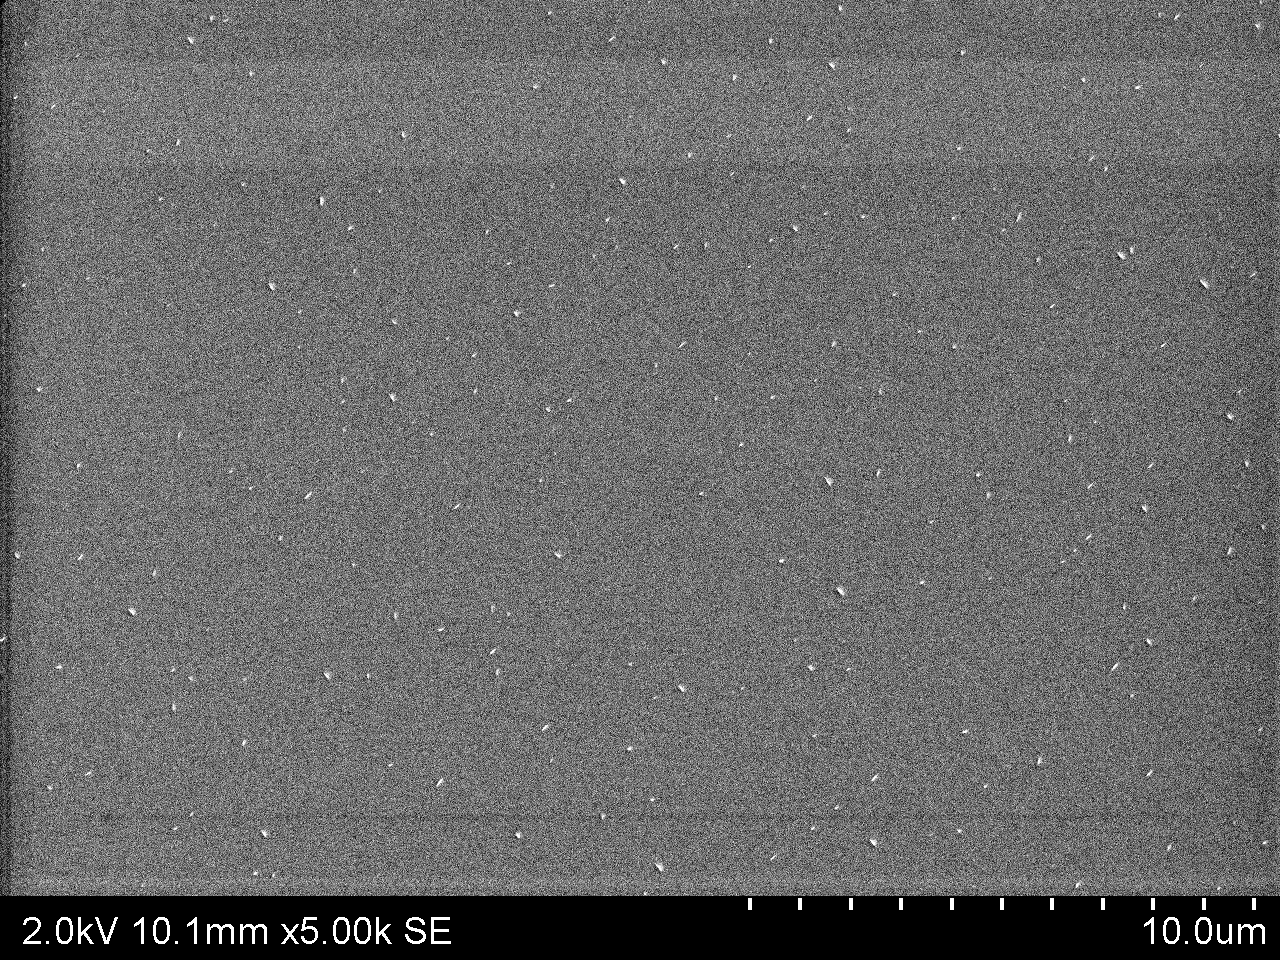
\includegraphics[width=1.0\linewidth]{sem_subCa_03_m005.png}
    \caption[\Ac{sem} image taken near the centre of the as-received substrate C.]{\Ac{sem} image taken near the centre of the as-received substrate C.}
    \label{fig:subCa_sem_area}
\end{figure}

An \ac{eds} spectrum of an agglomeration of particles with a diameter of \SI{50}{\nano\metre} revealed that the piece was composed of silica oxide, \ce{SiO2}, also known as silica, see Fig.~\ref{fig:subCa_polishing-grit}. As mentioned earlier, the presence of silica can be explained by the frequent use of silica as an abrasive in polishing slurries for semiconducting material. The \ce{Al} contamination that could be detected in the \ac{eds} spectrum obtained from a large area of the substrate can come from residual \ce{Al2O3} polishing grit, also known as alumina. Due to the small extent of the individual residual particles, it was not possible to get \ac{eds} spectra from them unless multiple particles formed a larger pile, which was rarely observed.

\begin{figure}[htbp]
    \centering
    \begin{subfigure}[t]{\textwidth}
        \caption{}\label{fig:subCa_polishing-grit}
          \begin{minipage}[c]{0.43\linewidth}
            \centering
            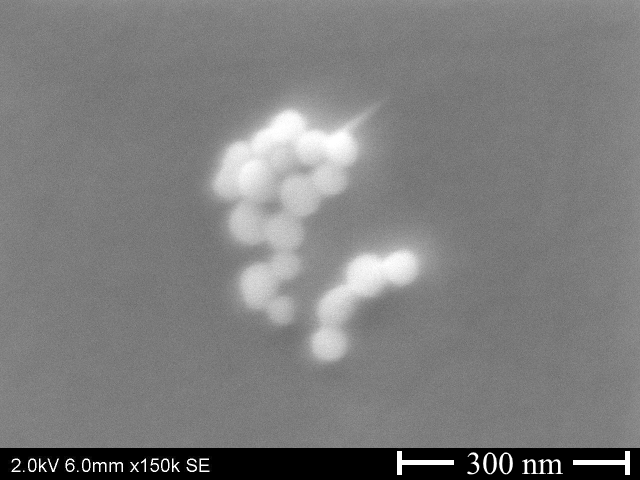
\includegraphics[width=\linewidth]{subCa_sem_09_m010.png}
          \end{minipage}
          \hfill
          \begin{minipage}[c]{0.43\linewidth}
            \centering
            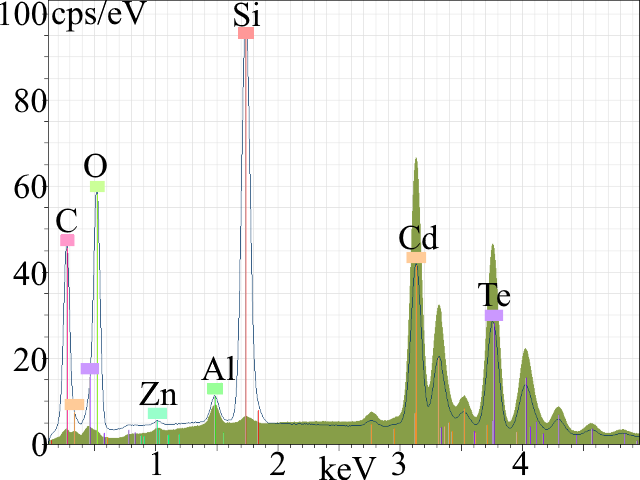
\includegraphics[width=\linewidth]{subCa_sem_09_m010_eds.png}
          \end{minipage}
          \begin{minipage}[c]{0.11\linewidth}
            \centering
            \atomicTable[\ce{O}&\SI{30.85}{}][\ce{C}&\SI{28.83}{}][\ce{Si}&\SI{22.20}{}][\ce{Cd}&\SI{8.61}{}][\ce{Te}&\SI{8.03}{}][\ce{Al}&\SI{1.28}{}][\ce{Zn}&\SI{0.20}{}]
          \end{minipage}
    \end{subfigure}%
    \par\bigskip
    \begin{subfigure}[t]{\textwidth}
        \caption{}\label{fig:subCa_carbon-based}
          \begin{minipage}[c]{0.43\linewidth}
            \centering
            \includegraphics[width=\linewidth]{sem_subCa_05_m011.jpg}
          \end{minipage}
          \hfill
          \begin{minipage}[c]{0.43\linewidth}
            \centering
            \includegraphics[width=\linewidth]{sem_subCa_05_m011_eds.png}
          \end{minipage}
          \begin{minipage}[c]{0.11\linewidth}
            \centering
            \atomicTable[\ce{C}&\SI{91.02}{}][\ce{O}&\SI{5.67}{}][\ce{N}&\SI{3.19}{}][\ce{Si}&\SI{0.11}{}]
          \end{minipage}
    \end{subfigure}%
    \caption[\Ac{sem} images, \ac{eds} spectra, and \ac{eds} atomic compositions of two different types of particles found on as-received substrate C.]{High resolution \ac{sem} images of two different types of particles found on the as-received substrate C and the corresponding \ac{eds} spectra and atomic compositions: \subref{fig:subCa_polishing-grit} silica (\ce{SiO2}), the blue spectrum represents the measurements from the particles, while the green spectrum represents the substrate surface next to the particles; and \subref{fig:subCa_carbon-based} carbon-based particle.}\label{fig:subCa_sem_w_eds}
\end{figure}

The polishing grit density was found to be between \SI{2e+06}{\centi\metre^{-2}} and \SI{1e+08}{\centi\metre^{-2}}. The average particle density was \SI{4e+07}{\centi\metre^{-2}} with a standard deviation of \SI{2e+07}{\centi\metre^{-2}}. A graphical representation of the particle density at different locations on substrate C can be seen in Fig.~\ref{fig:subCa_densityData}. This is in agreement with the results of \citet{benson2015as-received} who found that the silica polishing grit density varied from wafer-to-wafer from \SIrange{\sim5e6}{2e8}{\centi\metre^{-2}}.

\begin{figure}[htbp]
    \centering
    \includegraphics[width=0.7\linewidth]{subCa_densityData.png}
    \caption[Map of the polishing grit density on the as-received substrate C.]{A map of the polishing grit density at 24 different locations on the as-received $\SI{15}{\milli\metre}\times\SI{15}{\milli\metre}$ substrate C. The density measurements were obtained by counting the number of polishing grits in \ac{sem} images covering $\SI{25.4}{\micro\metre}\times\SI{17.8}{\micro\metre}$ areas. In total, \SI{0.005}{\percent} of the substrate surface was measured. The polishing grit density was observed to vary between \SI{2e+06}{\centi\metre^{-2}} and \SI{1e+08}{\centi\metre^{-2}}.}
    \label{fig:subCa_densityData}
\end{figure}

The large particles observed in the dark field images were infrequent with respect to the polishing grit. Only six were observed in the upper half of the substrate, which gives a density of \SI{\sim 3}{\centi\metre^{-2}}. The particles were typically between \SIrange{100}{500}{\micro\metre} long and \SIrange{20}{50}{\micro\metre} wide. The particles appeared darker than the surrounding substrate in the \ac{sem} images and the \ac{eds} spectra revealed that they were carbon-based, as seen in Fig.~\ref{fig:subCa_carbon-based}. As for the carbon-based particles on substrate B, these particles could be residue from mounting wax used during the polishing done by the vendor.

%%=========================================
%\section{AFM Study of As-Received Substrate C}
\subsection{Surface Roughness}
The as-received substrate C was characterised for surface topography by \ac{afm}. \Ac{afm} images of the substrate surface are shown in Fig.~\ref{fig:subCa_afm}. Polishing grit particles can be observed all over the surface of the substrate. The typical polishing grit density on the (211)B-oriented substrate is \SI{\sim 6e7 }{\centi\metre^{-2}}, which is in agreement with the density found from the \ac{sem} images. The typical polishing grit length was observed to be between \SIrange{50}{200}{\nano\metre} and the typical height was measured to be about \SI{\sim 10}{\nano\metre} above the (211)B surface. The small height above the surface compared to the diameter of the particles indicates that the polishing grit particles have penetrated the surface and are partly included in the surface.

\begin{figure}[htbp]
    \centering
    \begin{subfigure}[c]{0.032\linewidth}
        \label{fig:subCa_afm_scale}\captionsetup{list=no}
        \includegraphics[width=\linewidth]{subCa_afm_scale.png}
    \end{subfigure}
    \hfill
    \mySubfigure{0.3\linewidth}{subCa_afm_centre.png}[fig:subCa_afm_centre]%0,33\SI{0,28}{\nano\metre}
    \hfill
    \mySubfigure{0.3\linewidth}{subCa_afm_leftedge.png}[fig:subCa_afm_edge]%0,46 \SI{0,36}{\nano\metre}
    \hfill
    \mySubfigure{0.3\linewidth}{subCa_afm_upperleftcorner.png}[fig:subCa_afm_corner]% 0.54\SI{0,40}{\nano\metre}
    \caption[\Ac{afm} of as-received substrate C.]{\Ac{afm} measurements of the as-received substrate C. Images of $\SI{5}{\micro\metre}\times\SI{5}{\micro\metre}$ areas are taken at three different locations on the substrate surface: \subref{fig:subCa_afm_centre} near the centre, \ac{rms} roughness \SI{0.95}{\nano\metre}; \subref{fig:subCa_afm_edge} near the left edge, \ac{rms} roughness \SI{1.4}{\nano\metre}; and \subref{fig:subCa_afm_corner} near the upper left corner, \ac{rms} roughness \SI{1.4}{\nano\metre}.}
    \label{fig:subCa_afm}
\end{figure} % AFM, substrate C, as-received.

The \ac{rms} roughness was calculated to be \SI{0.95}{\nano\metre} near the centre, \SI{1.4}{\nano\metre} near the edge, and \SI{1.4}{\nano\metre} near the corner, using Eq.~\ref{eq:rmsroughness}. The polishing grit particles contributed to a higher roughness. To obtain \iac{rms} roughness of the substrate surface which was independent of the polishing grit density, measurements were performed on areas where there was no polishing grit. Several such measurements were performed within the same image. The average of the measurements resulted in \iac{rms} roughness of \SI{\sim 0,3}{\nano\metre} at the centre and \SI{\sim 0.5}{\nano\metre} around the edges. \citet{benson2015as-received} measured a similar \ac{rms} roughness of \SI{\sim 0.4}{\nano\metre} on all the as-received (211)B-oriented \ac{czt} substrates they studied. The low \ac{rms} roughness indicates an absence of deep scratches. The deepest observed polishing scratches on substrate C were \SI{0,2}{\micro\metre} wide and only \SI{1}{\nano\metre} deep. 

%\andreas{BOKMERKE}
Fig.~\ref{fig:sem-afm-comparison} show a comparison of an \ac{afm} image with a \ac{sem} image taken at the same location on the as-received substrate C. The same particle configuration can be seen in both images, but the shape and size of the polishing grit particles observed in \ac{afm} were different compared to what were observed in the \ac{sem} images. This image artifact in the \ac{afm} image can be explained by the convolution effect between the tip and the polishing grit particles, as described in Section~\ref{sec:afm}. In other words, due to a too-course tip, an image artifact occured in the \ac{afm} image that made the particles look wider and longer than they really were. 

\begin{figure}[htbp]
    \centering
    \mySubfigure{0.5\linewidth}{subCa_sem_afm_compare_m010.png}[fig:sem-afm-comparison_sem]
    \hfill\hfill
    \begin{subfigure}[c]{0.04\linewidth}
        \label{fig:subCa_afm_vs_sem_scale}\captionsetup{list=no}
        \includegraphics[width=\linewidth]{subCa_afm_vs_sem_scale.png}
    \end{subfigure}
    \hfill
    \mySubfigure{0.375\linewidth}{subCa_afm_vs_sem.png}[fig:sem-afm-comparison_afm]
    \caption[Comparison of an \ac{afm} image with a \ac{sem} image taken at the same location on substrate C.]{Comparison of \subref{fig:sem-afm-comparison_sem} a \ac{sem} image with \subref{fig:sem-afm-comparison_afm} an \ac{afm} image taken at the same location on the as-received substrate C. The height of the features in the \ac{afm} image is displayed as colour gradations. The same location with the same particles can be seen in both the \ac{afm} image and the \ac{sem} image, but due to a too-course tip, an image artifact occur in the \ac{afm} image that makes the particles look wider and longer than they are. The advantage of the \ac{afm} image is that it gives height information.}
    \label{fig:sem-afm-comparison}
\end{figure}

%\todo{Hvorfor er størrelsen og formen på partiklene sett med AFM helt ulik det sett i SEM? Er det to ulike typer partikler? Og i så fall, hvorfor ser jeg ikke poleringspartiklene i AFM? Og hvorfor ser jeg ikke hulrom med partikkel i midten i SEM? Er gropene for grunne (10 nm) til at de kan sees i SEM? Eller er det avbildingsfeil i AFM?}
%\begin{itemize}
%    \item \todo{Teori 1: To typer. AFM dytter vekk poleringspartiklene, SEM kan ikke se så grunne hulrom.}
%    \item \todo{Teori 2: Én type. AFM dytter vekk poleringspartiklene, det vi ser er slik det ser ut under poleringspartiklene. Denne teorien støttes av at alle gropene peker i samme retning.}
%    \item \todo{Teori 3: Én type. Det er samme type partikler vi ser i både SEM og AFM, men pga. avbildningsfeil i AFM, oppfattes de annerledes.}
%\end{itemize}

%%=========================================
\subsection{Impurity Analysis -- EDS}

\Ac{eds} impurity analysis was performed on the as-received substrate C. Three locations on the surface -- the centre, the edge, and the corner -- were analysed. The results of this analysis can be seen in Table~\ref{tab:subCa_eds_analysis}. The elements found above the \ac{eds} detection limit, in addition to \ce{Cd}, \ce{Zn}, and \ce{Te}, were \ce{Al}, \ce{Si}, \ce{C}, and \ce{O}. \ce{Si} and \ce{O} can be accounted for by silica polishing grit. Even though none of the polishing grit agglomerations contained alumina, it could be that some of the single grit that could not be measured using \ac{eds}, contained alumina and can account for the detection of \ce{Al}.

\begin{table}[htbp]
    \centering
    \caption[\Ac{eds} impurity analysis of the as-received substrate C.]{Results of the \ac{eds} impurity analysis at three different locations on the $\SI{15}{\milli\metre}\times\SI{15}{\milli\metre}$ as-received (211)B \ac{czt} substrate C (atomic concentration \%). The X-ray signal was acquired from $\SI{1270}{\micro\metre}\times\SI{890}{\micro\metre}$ areas near the centre, upper edge, and upper left corner.}\label{tab:subCa_eds_analysis}
    \begin{tabu} to 1.0\textwidth { X[1.85,r] X[1.125,c] X[1.125,c] X[1.125,c] X[1.125,c] X[1.125,c] X[1.125,c] X[1.125,c] }
    \hline
         & \textbf{\ce{Te}} (at.\%) & \textbf{\ce{Cd}} (at.\%) & \textbf{\ce{Zn}} (at.\%) & \textbf{\ce{Al}} (at.\%) & \textbf{\ce{Si}} (at.\%) & \textbf{\ce{C} } (at.\%) & \textbf{\ce{O}} (at.\%) \\
        \hline
        Near centre  & \SI{44.85}{}& \SI{44.90}{} & \SI{1.44}{} & \SI{1.98}{}& \SI{0.51}{} & \SI{4.93}{} & \SI{1.40}{}  \\ % \SI{7.5}{} & \SI{7.5}{}
        Near edge  & \SI{45.09}{}& \SI{45.09}{} & \SI{1.49}{} & \SI{1.70}{}& \SI{0.46}{} & \SI{4.93}{} & \SI{1.23}{}  \\ %\SI{7.5}{} & \SI{14.0}{}
         Near corner & \SI{45.05}{}& \SI{45.09}{} & \SI{1.44}{} & \SI{2.00}{}& \SI{0.46}{} & \SI{4.83}{} & \SI{1.13}{} \\ %\SI{1.0}{} & \SI{14.0}{}
         \hline
    \end{tabu}
\end{table}

%%=========================================
%\section{Near-IR of As-Received Substrate C}

%Near-\ac{ir} transmission microscopy images of as-received substrate C show a structure that has not appeared on either optical microscopy, \ac{sem}, or \ac{afm}. The structures are closed loops -- both circular loops and buckled loops with more curvature -- that appear brighter than the surrounding substrate, see Fig.~\ref{fig:subCa_irt}. The fact that the loops are brighter indicates that more of the photons are transmitted through. \todo{Også på (111)B fra samme leverandør? Kan vaskes vekk med acetone and methanole (?). Finnes det bedre bilde?}

%\begin{figure}[htbp]
%    \centering
%    \includegraphics[width=1.0\linewidth]{ir_20170210_038.jpg}
%    \caption[Near-\ac{ir} transmission microscopy of as-received substrate C.]{Near-\ac{ir} transmission microscopy images of as-received substrate C taken near the lower left corner.}
%    \label{fig:subCa_irt}
%\end{figure}

%%=========================================
% FTIR transmission spectra
\subsection{IR Characterisation}

\Ac{ftir} transmission spectra were recorded from a $5\times5$ grid on the as-received substrate C. The grid points were placed \SI{2.3}{\milli\metre} from the edge and had \SI{2.6}{\milli\metre} between nearest neighbours. All but five spectra had the same characteristics as substrate A, see Fig.~\ref{fig:subCa_ftir_spectra}, and hence, have the same properties regarding precipitates, carrier concentration, and resistivity as substrate A \citep{yujie2004infrared}.

\begin{figure}[htbp]
    \centering
    \mySubfigure{0.60175438596\linewidth}{subCa_25_ftir_spectra.png}[fig:subCa_ftir_spectra]
    \hfill
    \mySubfigure{0.37824561403\linewidth}{subCa_25_ftir_transmission_at_k500cm-1.png}[fig:subCa_ftir_map_500cm-1]
    \caption[\Ac{ftir} measurements of the as-received substrate C.]{\Ac{ftir} measurements recorded from a $5\times5$ grid on the as-received $\SI{15}{\milli\metre}\times\SI{15}{\milli\metre}$ (211)B-oriented substrate C: \subref{fig:subCa_ftir_spectra} Transmission spectra; and \subref{fig:subCa_ftir_map_500cm-1} transmission map at wavenumber $k=\SI{500}{\centi\metre^{-1}}$ showing the transmittance $T$ in percentage of incoming light at each grid point. The spikes near $k=\SI{4500}{\centi\metre^{-1}}$ and $k=\SI{5000}{\centi\metre^{-1}}$ were artefacts of the \ac{ftir} instrument.}
\end{figure}

The five measurements obtained from the upper edge of substrate C had transmittance between \SI{55}{\percent} and \SI{61}{\percent} in the wavenumber region of interest, which are lower than for the rest of the substrate, see Fig.~\ref{fig:subCa_ftir_map_500cm-1}. Apart from having lower transmission they have the same shape and similar $T_{1000}/T_{5000}$ indicator as the other spectra. For this reason, and the fact that the lower transmission occur only at the upper edge, it is believed that the frame that holds the substrate obscure the light at the upper edge, and results in an overall lower transmission (E. Selvig, personal communication, May 24, 2017). Taking this into account, the spectra from the upper edge have the same characteristics as the rest.
%and the indicator $T_{1000}/T_{5000}$ tends to be a little bit larger than one for these points. According to \citet{yujie2004infrared}, the \ac{czt} substrates with these characteristics have a high density of tiny and dense \ce{Te} precipitates, high free carrier concentrations, and a resistivity less than \SI{500}{\ohm\centi\metre}.



%%=========================================
%\clearpage
%%=========================================
% Den litt rare section-formuleringen er for å en kortere header-tittel siden den er for lang ellers.
% \sectionmark{} inne i {section title as seen in paper ...} er for å få riktig header der en section begynner på en oddetallsside.
%
%   \section[section title as seen in TOC]{section title as seen in paper%
%       \sectionmark{section title as seen in header}}\sectionmark{section title as seen in header}
%
\section[Surface Analysis of Substrate A with Surface Pre-Growth Preparation]{Surface Analysis of Substrate A with Surface Pre-Growth Preparation%
    \sectionmark{Surface Analysis of Pre-Growth Substrate A}}\sectionmark{Surface Analysis of Pre-Growth Substrate A}\label{sec:subAb}


%%=========================================
\subsection{Particles}

\begin{figure}
    \centering
    \begin{subfigure}[t]{\textwidth}
          \begin{minipage}[t]{0.49\linewidth}
            \centering
            \includegraphics[width=\linewidth]{unknown.png}
          \end{minipage}
          \hspace{0.02\linewidth}
          \begin{minipage}[t]{0.49\linewidth}
            \centering
            \includegraphics[width=\linewidth]{unknown.png}
          \end{minipage}
        \caption{\todo{Add caption}}\label{fig:add_label}
    \end{subfigure}
    \par\bigskip
    \begin{subfigure}[t]{\textwidth}
          \begin{minipage}[t]{0.49\linewidth}
            \centering
            \includegraphics[width=\linewidth]{unknown.png}
          \end{minipage}
          \hspace{0.02\linewidth}
          \begin{minipage}[t]{0.49\linewidth}
            \centering
            \includegraphics[width=\linewidth]{unknown.png}
          \end{minipage}
        \caption{\todo{Add caption}}\label{fig:add_label}
    \end{subfigure}
    \par\bigskip
    \begin{subfigure}[t]{\textwidth}
          \begin{minipage}[t]{0.49\linewidth}
            \centering
            \includegraphics[width=\linewidth]{unknown.png}
          \end{minipage}
          \hspace{0.02\linewidth}
          \begin{minipage}[t]{0.49\linewidth}
            \centering
            \includegraphics[width=\linewidth]{unknown.png}
          \end{minipage}
        \caption{\todo{Add caption}}\label{fig:add_label}
    \end{subfigure}
    \caption[\Ac{sem} images and \ac{eds} spectra of particles found on substrate A after surface pre-growth preparation.]{High resolution \acf{sem} images of particles found on substrate A after surface pre-growth preparation and the corresponding \acf{eds} spectra of the particles.}\label{fig:subAb_sem_w_eds}
\end{figure}

\begin{figure}[htbp]
\ContinuedFloat
    \centering
    \begin{subfigure}[t]{\textwidth}
          \begin{minipage}[t]{0.49\linewidth}
            \centering
            \includegraphics[width=\linewidth]{unknown.png}
          \end{minipage}
          \hspace{0.02\linewidth}
          \begin{minipage}[t]{0.49\linewidth}
            \centering
            \includegraphics[width=\linewidth]{unknown.png}
          \end{minipage}
        \caption{\todo{Add caption}}\label{fig:add_label}
    \end{subfigure}
    \captionsetup{list=no}
    \caption{\emph{(continued)}}
\end{figure}


%%=========================================
%\section{AFM Study of Etched Substrate A}
\subsection{Surface Roughness}

\begin{figure}[htbp]
    \centering
    \begin{subfigure}[t]{\linewidth}
        \centering
        \includegraphics[width=0.5\linewidth,trim={0cm 12cm 21cm 0cm},clip]{170502Topography014_centre.png}
        \caption{Near centre, \ac{rms} roughness \SI{0.5}{\nano\metre}.} %\SI{0.85}{\nano\metre}
    \end{subfigure}%
    \par\bigskip
    \begin{subfigure}[t]{\linewidth}
        \centering
        \includegraphics[width=0.5\linewidth,trim={0cm 12cm 21cm 0cm},clip]{170502Topography010_upperedge.png}
        \caption{Near upper edge, \ac{rms} roughness \SI{1.3}{\nano\metre}.} %\SI{0.77}{\nano\metre}}
    \end{subfigure}%
    \par\bigskip
    \begin{subfigure}[t]{\linewidth}
        \centering
        \includegraphics[width=0.5\linewidth,trim={0cm 12cm 21cm 0cm},clip]{170502Topography006_upperleftcorner.png}
        \caption{Near upper left corner, \ac{rms} roughness \SI{1.9}{\nano\metre}.}\SI{1,04}{\nano\metre}
    \end{subfigure}%
    \caption[\Ac{afm} of substrate A with surface pre-growth preparation.]{\Acf{afm} measurements of substrate A with surface pre-growth preparation. Images of a $\SI{5}{\micro\metre}\times\SI{5}{\micro\metre}$ area are taken at the centre, edge, and corner of the substrate.}\label{fig:afm_subAb}
\end{figure} % AFM, substrate A, with surface pre-growth preparation.

%%=========================================
\subsection{Impurity Analysis}

\begin{table}[htbp]
    \centering
    \caption[\Ac{eds} impurity analysis of substrate A with surface pre-growth preparation.]{Results of the \acf{eds} impurity analysis at three different locations on the $30\times30$ \SI{}{\milli\metre^2} (111)B \ac{czt} substrate A with surface pre-growth preparation (atomic concentration \%). The X-ray signal is acquired from a $\SI{1270}{}\times\SI{890}{\micro\metre^2}$ area centred around the given $X$ and $Y$ values at a magnification of 100$\times$.}\label{tab:subAb_eds_analysis}
   \begin{tabu} to 1.0\textwidth { X[1,c] X[1,c] X[1.125,c] X[1.125,c] X[1.125,c] X[1.125,c] X[1.125,c] X[1.125,c] X[1.125,c] }
    \hline
        \textbf{$X$} (\SI{}{\milli\metre}) &  \textbf{$Y$} (\SI{}{\milli\metre}) & \textbf{\ce{Te}} (at.\%) & \textbf{\ce{Cd}} (at.\%) & \textbf{\ce{Zn}} (at.\%) & \textbf{\ce{Al} } (at.\%) & \textbf{\ce{Si}} (at.\%) & \textbf{\ce{C}} (at.\%) & \textbf{\ce{O}} (at.\%) \\
        \hline
         \SI{1.0}{}  & \SI{29.0}{} & \SI{}{} & \SI{}{} & \SI{}{} & \SI{}{} & \SI{}{} & \SI{}{} & \SI{}{} \\
         \SI{15.0}{} & \SI{29.0}{} & \SI{}{} & \SI{}{} & \SI{}{} & \SI{}{} & \SI{}{} & \SI{}{} & \SI{}{} \\
         \SI{15.0}{} & \SI{15.0}{} & \SI{}{} & \SI{}{} & \SI{}{} & \SI{}{} & \SI{}{} & \SI{}{} & \SI{}{} \\
         \hline
    \end{tabu}
\end{table}
%%=========================================


%\clearpage
%%=========================================
\section[Surface Analysis of Substrate B with Surface Pre-Growth Preparation]{Surface Analysis of Substrate B with Surface Pre-Growth Preparation%
   \sectionmark{Surface Analysis of Pre-Growth Substrate B}}\sectionmark{Surface Analysis of Pre-Growth Substrate B}\label{sec:subBb}
   
The dark field images taken of the surface of substrate B after polishing and an etch show that the surface pre-growth preparation has improved the surface considerably, see Fig.~\ref{fig:subBa_om_df} and Fig.~\ref{fig:subBb_om_df}. The previously observed deep surface scratches are removed and there are far less particles on the substrate surface.

\begin{figure}[htbp]
    \centering
    \includegraphics[width=0.8\linewidth]{subBb_om_n030.jpg}
    \caption[Dark field optical microscopy image of substrate B with surface pre-growth preparation.]{Dark field optical microscopy image of substrate B with surface pre-growth preparation taken in the upper left corner of the substrate at a magnification of $20\times$. The same particle configuration can be observed in both images.}
    \label{fig:subBb_om_df}
\end{figure}
   
   
%%=========================================
   
\begin{figure}[htbp]
    \centering
    \includegraphics[width=0.8\linewidth]{unknown.png}
    \caption[\Ac{sem} of the centre of substrate B with surface pre-growth preparation.]{\Acf{sem} image taken at the centre of substrate C after surface pre-growth preparation at a  magnification of $5000\times$.}
    \label{fig:subBb_sem_area}
\end{figure}

The surface of substrate B after preparation polish and etch \todo{}. However, there are many tiny particles with lengths of \SIrange{20}{50}{\nano\metre} on the substrate surface. A typical area in the centre of substrate B can be seen in Fig.~\ref{fig:subBb_sem_area}.

The small particles observed in \ac{sem} are distributed evenly over the surface with a tendency of higher density towards the upper right, lower right, and lower left corners. The particle density was found to be between \SI{5e+06}{\particle\centi\metre^{-2}} and \SI{5e+07}{\particle\centi\metre^{-2}}. The mean particle density was \SI{2e+07}{\particle\centi\metre^{-2}} with a standard deviation of \SI{9e+06}{\particle\centi\metre^{-2}}. A graphical representation of the particle density at different locations on substrate C can be seen in Fig.~\ref{fig:subBb_densityData}.

\begin{figure}[htbp]
    \centering
    \includegraphics[width=0.8\linewidth]{subBb_densityData.png}
    \caption[Map of the polishing grit density on substrate B after surface pre-growth preparation.]{A map of the polishing grit density at 121 different locations on the $\SI{30}{\milli\metre}\times\SI{30}{\milli\metre}$ substrate B after surface pre-growth preparation. The polishing grit density was observed to vary between \SI{5e+06}{\particle\centi\metre^{-2}} and \SI{5e+07}{\particle\centi\metre^{-2}}.}
    \label{fig:subBb_densityData}
\end{figure}

%%=========================================
\subsection{Particles}
\begin{figure}
    \centering
    \begin{subfigure}[t]{\textwidth}
          \begin{minipage}[t]{0.49\linewidth}
            \centering
            \includegraphics[width=\linewidth]{unknown.png}
          \end{minipage}
          \hspace{0.02\linewidth}
          \begin{minipage}[t]{0.49\linewidth}
            \centering
            \includegraphics[width=\linewidth]{unknown.png}
          \end{minipage}
        \caption{\todo{Add caption}}\label{fig:add_label}
    \end{subfigure}
    \par\bigskip
    \begin{subfigure}[t]{\textwidth}
          \begin{minipage}[t]{0.49\linewidth}
            \centering
            \includegraphics[width=\linewidth]{unknown.png}
          \end{minipage}
          \hspace{0.02\linewidth}
          \begin{minipage}[t]{0.49\linewidth}
            \centering
            \includegraphics[width=\linewidth]{unknown.png}
          \end{minipage}
        \caption{\todo{Add caption}}\label{fig:add_label}
    \end{subfigure}
    \par\bigskip
    \begin{subfigure}[t]{\textwidth}
          \begin{minipage}[t]{0.49\linewidth}
            \centering
            \includegraphics[width=\linewidth]{unknown.png}
          \end{minipage}
          \hspace{0.02\linewidth}
          \begin{minipage}[t]{0.49\linewidth}
            \centering
            \includegraphics[width=\linewidth]{unknown.png}
          \end{minipage}
        \caption{\todo{Add caption}}\label{fig:add_label}
    \end{subfigure}
    \caption[\Ac{sem} images and \ac{eds} spectra of particles found on substrate B after surface pre-growth preparation.]{High resolution \acf{sem} images of particles found on substrate B after surface pre-growth preparation and the corresponding \acf{eds} spectra of the particles.}\label{fig:subBb_sem_w_eds}
\end{figure}

\begin{figure}[htbp]
\ContinuedFloat
    \centering
    \begin{subfigure}[t]{\textwidth}
          \begin{minipage}[t]{0.49\linewidth}
            \centering
            \includegraphics[width=\linewidth]{unknown.png}
          \end{minipage}
          \hspace{0.02\linewidth}
          \begin{minipage}[t]{0.49\linewidth}
            \centering
            \includegraphics[width=\linewidth]{unknown.png}
          \end{minipage}
        \caption{\todo{Add caption}}\label{fig:add_label}
    \end{subfigure}
    \captionsetup{list=no}
    \caption{\emph{(continued)}}
\end{figure}


%%=========================================

%%=========================================
%\section{AFM Study of Polished and Etched Substrate B}
\subsection{Surface Roughness}
\begin{figure}[htbp]
    \centering
    \begin{subfigure}[t]{\linewidth}
    \centering
        \includegraphics[width=0.5\linewidth,trim={0cm 12cm 21cm 0cm},clip]{170405Topography008_centre.png}
        \caption{Near centre, \ac{rms} roughness \SI{0.9}{\nano\metre}.}%\SI{0.85}{\nano\metre}
    \end{subfigure}%
    \par\bigskip
    \begin{subfigure}[t]{\linewidth}
    \centering
        \includegraphics[width=0.5\linewidth,trim={0cm 12cm 21cm 0cm},clip]{170405Topography014_leftedge.png}
        \caption{[Near left edge, \ac{rms} roughness \SI{0.8}{\nano\metre}.}%\SI{0.77}{\nano\metre}
    \end{subfigure}%
    \par\bigskip
    \begin{subfigure}[t]{\linewidth}
    \centering
        \includegraphics[width=0.5\linewidth,trim={0cm 12cm 21cm 0cm},clip]{170405Topography018_upperleftcorner.png}
        \caption{Near upper left corner, \ac{rms} roughness \SI{0.9}{\nano\metre}.} %\SI{1,04}{\nano\metre}}
    \end{subfigure}%
    \caption[\Ac{afm} of substrate B with surface pre-growth preparation.]{\Acf{afm} measurements of substrate B with surface pre-growth preparation. Images of a $\SI{5}{\micro\metre}\times\SI{5}{\micro\metre}$ area are taken at the centre, edge, and corner of the substrate.}\label{fig:afm_subBb}
\end{figure} % AFM, substrate B, with surface pre-growth preparation.

%%=========================================
\subsection{Impurity Analysis}
\begin{table}[htbp]
    \centering
    \caption[\Ac{eds} impurity analysis of substrate B with surface pre-growth preparation.]{Results of the \acf{eds} impurity analysis at three different locations on the $30\times30$ \SI{}{\milli\metre^2} (111)B \ac{czt} substrate B with surface pre-growth preparation (atomic concentration \%). The X-ray signal is acquired from a $\SI{1270}{}\times\SI{890}{\micro\metre^2}$ area centred around the given $X$ and $Y$ values at a magnification of 100$\times$.}\label{tab:subBb_eds_analysis}
    \begin{tabu} to 1.0\textwidth { X[1,c] X[1,c] X[1.125,c] X[1.125,c] X[1.125,c] X[1.125,c] X[1.125,c] X[1.125,c] X[1.125,c] }
    \hline
        \textbf{$X$} (\SI{}{\milli\metre}) &  \textbf{$Y$} (\SI{}{\milli\metre}) & \textbf{\ce{Te}} (at.\%) & \textbf{\ce{Cd}} (at.\%) & \textbf{\ce{Zn}} (at.\%) & \textbf{\ce{Al} } (at.\%) & \textbf{\ce{Si}} (at.\%) & \textbf{\ce{C}} (at.\%) & \textbf{\ce{O}} (at.\%) \\
        \hline
         \SI{1.0}{}  & \SI{29.0}{} & \SI{45.83}{} & \SI{45.34}{} & \SI{1.92}{} & \SI{0.60}{} & \SI{0.50}{} & \SI{5.34}{} & \SI{0.47}{} \\
         \SI{15.0}{} & \SI{29.0}{} & \SI{45.49}{} & \SI{45.12}{} & \SI{2.02}{} & \SI{0.26}{} & \SI{0.49}{} & \SI{5.99}{} & \SI{0.64}{} \\
         \SI{15.0}{} & \SI{15.0}{} & \SI{46.10}{} & \SI{45.35}{} & \SI{1.92}{} & \SI{0.23}{} & \SI{0.52}{} & \SI{5.49}{} & \SI{0.40}{} \\
         \hline
    \end{tabu}
\end{table}
%%=========================================
% FTIR transmission spectra.
\subsection{IR Characterisation}
%%=========================================

%\clearpage
%%=========================================
\section[Surface Analysis of Substrate C with Surface Pre-Growth Preparation]{Surface Analysis of Substrate C with Surface Pre-Growth Preparation%
    \sectionmark{Surface Analysis of Pre-Growth Substrate C}}\sectionmark{Surface Analysis of Pre-Growth Substrate C}\label{sec:subCb}

The ultimate goal for the \ac{mbe} preparation etch is to provide a clean, smooth, and well-ordered surface to minimise growth defects.

%%=========================================
\subsection{Particles}

\begin{figure}
    \centering
    \begin{subfigure}[t]{\textwidth}
          \begin{minipage}[t]{0.49\linewidth}
            \centering
            \includegraphics[width=\linewidth]{unknown.png}
          \end{minipage}
          \hspace{0.02\linewidth}
          \begin{minipage}[t]{0.49\linewidth}
            \centering
            \includegraphics[width=\linewidth]{unknown.png}
          \end{minipage}
        \caption{\todo{Add caption}}\label{fig:add_label}
    \end{subfigure}
    \par\bigskip
    \begin{subfigure}[t]{\textwidth}
          \begin{minipage}[t]{0.49\linewidth}
            \centering
            \includegraphics[width=\linewidth]{unknown.png}
          \end{minipage}
          \hspace{0.02\linewidth}
          \begin{minipage}[t]{0.49\linewidth}
            \centering
            \includegraphics[width=\linewidth]{unknown.png}
          \end{minipage}
        \caption{\todo{Add caption}}\label{fig:add_label}
    \end{subfigure}
    \par\bigskip
    \begin{subfigure}[t]{\textwidth}
          \begin{minipage}[t]{0.49\linewidth}
            \centering
            \includegraphics[width=\linewidth]{unknown.png}
          \end{minipage}
          \hspace{0.02\linewidth}
          \begin{minipage}[t]{0.49\linewidth}
            \centering
            \includegraphics[width=\linewidth]{unknown.png}
          \end{minipage}
        \caption{\todo{Add caption}}\label{fig:add_label}
    \end{subfigure}
    \caption[\Ac{sem} images and \ac{eds} spectra of particles found on substrate C after surface pre-growth preparation.]{High resolution \acf{sem} images of particles found on substrate C after surface pre-growth preparation and the corresponding \acf{eds} spectra of the particles.}\label{fig:subCb_sem_w_eds}
\end{figure}

\begin{figure}[htbp]
\ContinuedFloat
    \centering
    \begin{subfigure}[t]{\textwidth}
          \begin{minipage}[t]{0.49\linewidth}
            \centering
            \includegraphics[width=\linewidth]{unknown.png}
          \end{minipage}
          \hspace{0.02\linewidth}
          \begin{minipage}[t]{0.49\linewidth}
            \centering
            \includegraphics[width=\linewidth]{unknown.png}
          \end{minipage}
        \caption{\todo{Add caption}}\label{fig:add_label}
    \end{subfigure}
    \captionsetup{list=no}
    \caption{\emph{(continued)}}
\end{figure}

\todo{The alumina polishing grit observed in \ac{sem} are found all over the surface with a tendency of higher density towards the upper right, lower right, and lower left corners. The particle density was found to be between \SI{5e+06}{\particle\centi\metre^{-2}} and \SI{3e+07}{\particle\centi\metre^{-2}}. The mean particle density was \SI{2e+07}{\particle\centi\metre^{-2}} with a standard deviation of \SI{7e+06}{\particle\centi\metre^{-2}}. A graphical representation of the particle density at 25 different locations on substrate C can be seen in Fig.~\ref{fig:subCb_densityData}.}

\begin{figure}[htbp]
    \centering
    \includegraphics[width=0.8\linewidth]{subCb_densityData.png}
    \caption[Map of the polishing grit density on substrate C after surface pre-growth preparation.]{A map of the polishing grit density at 25 different locations on the $\SI{15}{\milli\metre}\times\SI{15}{\milli\metre}$ substrate C after surface pre-growth preparation. The polishing grit density was observed to vary between \todo{\SI{5e+06}{\particle\centi\metre^{-2}} and \SI{3e+07}{\particle\centi\metre^{-2}}}.}
    \label{fig:subCb_densityData}
\end{figure}


%%=========================================
%\section{AFM Study of Etched Substrate C}
\subsection{Surface Roughness}
\begin{figure}[htbp]
    \centering
    \begin{subfigure}[t]{\linewidth}
    \centering
        \includegraphics[width=0.5\linewidth,trim={0cm 12cm 21cm 0cm},clip]{170428Topography002_centre.png}
        \caption{Near centre, \ac{rms} roughness \SI{1.4}{\nano\metre}.}  %\SI{0.85}{\nano\metre}}
    \end{subfigure}%
    \par\bigskip
    \begin{subfigure}[t]{\linewidth}
    \centering
        \includegraphics[width=0.5\linewidth,trim={0cm 12cm 21cm 0cm},clip]{170427Topography016_upperedge.png}
        \caption{Near upper edge, \ac{rms} roughness \SI{1.4}{\nano\metre}.}  %\SI{0.77}{\nano\metre}}
    \end{subfigure}%
    \par\bigskip
    \begin{subfigure}[t]{\linewidth}
    \centering
        \includegraphics[width=0.5\linewidth,trim={0cm 12cm 21cm 0cm},clip]{170427Topography012_upperleftcorner.png}
        \caption{Near upper left corner, \ac{rms} roughness \SI{2.8}{\nano\metre}.}  %\SI{1,04}{\nano\metre}}
    \end{subfigure}%
    \caption[\Ac{afm} of substrate C with surface pre-growth preparation.]{\Acf{afm} measurements of substrate C with surface pre-growth preparation. Images of a $\SI{5}{\micro\metre}\times\SI{5}{\micro\metre}$ area are taken at the centre, edge, and corner of the substrate.}
    \label{fig:afm_subCb}
\end{figure} % AFM, substrate C, with surface pre-growth preparation.

%%=========================================
\subsection{Impurity Analysis}
\begin{table}[htbp]
    \centering
    \caption[\Ac{eds} impurity analysis of substrate C with surface pre-growth preparation.]{Results of the \acf{eds} impurity analysis at three different locations on the $15\times15$ \SI{}{\milli\metre^2} (211)B \ac{czt} substrate C with surface pre-growth preparation (atomic concentration \%). The X-ray signal is acquired from a $\SI{1270}{}\times\SI{890}{\micro\metre^2}$ area centred around the given $X$ and $Y$ values at a magnification of 100$\times$.}\label{tab:subCb_eds_analysis}
    \begin{tabu} to 1.0\textwidth { X[1,c] X[1,c] X[1.125,c] X[1.125,c] X[1.125,c] X[1.125,c] X[1.125,c] X[1.125,c] X[1.125,c] }
    \hline
        \textbf{$X$} (\SI{}{\milli\metre}) &  \textbf{$Y$} (\SI{}{\milli\metre}) & \textbf{\ce{Te}} (at.\%) & \textbf{\ce{Cd}} (at.\%) & \textbf{\ce{Zn}} (at.\%) & \textbf{\ce{Al} } (at.\%) & \textbf{\ce{Si}} (at.\%) & \textbf{\ce{C}} (at.\%) & \textbf{\ce{O}} (at.\%) \\
        \hline
         \SI{1.0}{} & \SI{14.0}{} & \SI{45.16}{} & \SI{45.26}{} & \SI{1.40}{} & \SI{1.79}{} & \SI{0.54}{} & \SI{5.85}{} & \SI{0}{} \\
         \SI{7.5}{} & \SI{14.0}{} & \SI{44.91}{} & \SI{44.93}{} & \SI{1.43}{} & \SI{2.33}{} & \SI{0.53}{} & \SI{5.86}{} & \SI{0}{} \\
         \SI{7.5}{} & \SI{7.5}{}  & \SI{45.02}{} & \SI{44.88}{} & \SI{1.45}{} & \SI{2.14}{} & \SI{0.52}{} & \SI{6.00}{} & \SI{0}{} \\
         \hline
    \end{tabu}
\end{table}

%%=========================================
%\clearpage
%%=========================================
\section{Comparison of the Substrates}\label{sec:comparison}

A summary of the different particle types and defects that have been observed on the substrate surfaces can be seen in Table~\ref{tab:particle_comparison}.

\begin{table}[htbp]
    \centering
    \caption[Comparison of the four \ac{czt} substrates.]{Comparison of the four \ac{czt} substrates which have been studied. The density of the observed particles are given for the substrates both as-received and with surface pre-growth preparation (\SI{}{\centi\metre^{-2}}). A dash (---) marks the cases where there was not observed any of the given particle type.}\label{tab:particle_comparison}
    \begin{tabu} to 1.0\textwidth { >{\bfseries} X[1.2,c] X[1,c] X[1,c] X[1,c] X[1,c] X[1,c] X[1,c] X[1,c] }
    \hline
        %& \textbf{Substrate A As-received} &  \textbf{Substrate A With surface pre-growth preparation} & \textbf{Substrate B As-received} &  \textbf{Substrate B With surface pre-growth preparation} & \textbf{Substrate B2 With surface pre-growth preparation} & \textbf{Substrate C As-received} &  \textbf{Substrate C With surface pre-growth preparation}\\
        & \shortstack{\textbf{A}\\\scriptsize{as-received}} &  \shortstack{\textbf{A}\\\scriptsize{pre-growth}} & \shortstack{\textbf{B}\\\scriptsize{as-received}} &  \shortstack{\textbf{B}\\\scriptsize{pre-growth}} & \shortstack{\textbf{B2}\\\scriptsize{pre-growth}} & \shortstack{\textbf{C}\\\scriptsize{as-received}} &  \shortstack{\textbf{C}\\\scriptsize{pre-growth}} \\
        %                   &   Aa     &    Ab   &   Ba    &    Bb   &    B2b   &   Ca    &    Cb   \\
        \hline
        Polishing grit  &\SI{<2e4}{}&\SI{1e6}{}&&\SI{5e6}{}&\SI{8e6}{}&\SI{4e7}{}&\SI{1e6}{}\\
        \ce{CdZnTe}     &      &       &       &       &       &       &       \\
        \ce{C}-based    & ---    &       &       &       &       &       &       \\
         &       &       &       &       &       &       &       \\
         &       &       &       &       &       &       &       \\
         &       &       &       &       &       &       &       \\
        \hline
    \end{tabu}
\end{table}



%%=========================================
%%%=========================================
\chapter{Conclusions}\label{ch:conclusion}
% In this final chapter you should sum up what you have done and which results you have got. You should also discuss your findings, and give recommendations for further work.
% Here, you present a brief summary of your work and list the main results you have got. You should give comments to each of the objectives in Chapter 1 and state whether or not you have met the objective. If you have not met the objective, you should explain why (e.g., data not available, too difficult). This section is similar to the Summary and Conclusions in the beginning of your report, but more detailed—referring to the the various sections in the report.


%The findings in this report confirm that the TMDCs are strongly interacting, and further understanding of the interactions and control of these systems could pave the way for spintronics for a new generation of multifunctional electronic devices. % Fin overgang til neste kapittel som er "further work".

%%%=========================================
\chapter{Further Work}\label{ch:further-work}
% You should give recommendations to possible extensions to your work. The recommendations should be as specific as possible, preferably with an objective and an indication of a possible approach.
%A further line of study based on concepts studied in this thesis would be a more in depth study of the 

%\mycomment{Skriv om ulike overflatebehandlinger, mulighet for å bruke nær-IR mikroskopi.}
% The recommendations may be classified as:
% • Short-term
% • Medium-term
% • Long-term
%%=========================================

Finne metode for å bli kvitt partikler fra kantene på vendor A substrat alik at de ikke løses opp i etsen og legger seg ned på substratoverflaten. Metode for å etse uten å legge igjen så mye partikler (1) ha en skillevegg i etsebegeret slik at en kan etse i det ene kammeret og så ta opp av væsken på andre siden av en glassvegg. Tendens til at partikler legger seg i overflaten, 2) noen løsemidler er bedre til å ta opp og vekk partikler enn andre.)

Studere lav transmisjon og om det gir lysere områder i SEM og alltid eller bare der p-doping. Mørkere n-doping?

Correlate the density of donuts with the density of tellurium precipitates near the surface.


%%%=========================================
\chapter{Results and Discussion}
In this chapter, experimental results are presented, analysed and discussed. In total, two substrates from different vendors were investigated using dark field microscopy, \ac{sem}, \ac{eds} and \ac{xps}.
%%=========================================
\section{Substrate Overview}

As observed in the \ac{sem} images in figure~\ref{fig:SEM_corners}, substrate B has an imperfect perpendicular edge with a lot of indents and marks while substrate A has a bevelled edge that extends approximately \SI{180}{\micro\metre} from the edge onto the substrate surface. Approximately \SI{140}{\micro\metre} from the edge of substrate A there is a band of cavities in the surface before the last \SI{40}{\micro\metre} of the rim is curved gradually to meet the flat substrate surface.

\begin{figure}[htbp]
    \centering
    \subfigure[SEM image of the southeast corner of substrate A at a magnification of 300$\times$.]{\includegraphics[width=0.48\linewidth]{SEM_BZ1503A_b_m008.jpg}}
    \quad
    \subfigure[SEM image of the southwest corner of substrate B at a magnification of 300$\times$.]{\includegraphics[width=0.48\linewidth]{20161214_C389523A_corners_m004.jpg}}
    \caption[SEM images of the corners on the substrates.]{Scanning electron microscopy (SEM) images of a corner on the two substrates taken at a magnification of 300$\times$.}
    \label{fig:SEM_corners}
\end{figure}


%%=========================================
\section{EDS Analysis of As-Received Substrates}

\Ac{eds} was performed on the substrates to determine the composition of the surface layers. Three areas on the substrates were analysed: the centre, \SI{1}{\milli\metre} from the centre of the upper edge, and \SI{1}{\milli\metre} from each of the edges of the the upper left corner. The analysis depth of \ac{eds} at \SI{12}{\kilo\volt} is about \SI{700}{\nano\metre}. As one monolayer of \ac{czt} is \SI{\sim 6.5}{\angstrom}, this implies that the result covers much more than the outermost surface layers. The quantitative result is an average elemental composition of the volume that is analysed.

\todo{Plasser et annet seted.} Ideally, \ac{xps} analysis, which has an analysis depth of \SI{\sim 80}{\angstrom} for \ac{mct}, should be performed on the substrates in order to determine the composition of the outermost layers of the substrates. Unfortunately, something was broken on the old analyser at \ac{ffi}, resulting in low signal intensity and no detection of impurities or small concentrations of elements. The ever-present oxide and carbon overlayers further decreased any small signals. Therefore, the XPS only gave information about the following elements: \ce{Te}, \ce{Cd}, \ce{O}, and \ce{C}. The reason for not performing \ac{xps} analysis on other than the as-received substrate A was that it would not be possible to detect the presence of impurities or small concentrations of elements with the \ac{xps} equipment at hand.

%\todo{Plagiat av meg selv?} The atomic concentrations was calculated using Eq.~\eqref{eq:xps_concentration} with intensity peak areas and the following experimentally measured atomic sensitivity factors, determined by \citet{hirsch1999x-ray}: \ce{Cd} 3d\textsubscript{5/2} (0.56), \ce{Te} 3d\textsubscript{5/2} (1.00), \ce{O} 1s (0.13), and \ce{C} 1s (0.05). Table~\ref{tab:xps_results} displays the results of the \ac{xps} analysis of the as-received substrate A. \ce{Cd_{0.96}Zn_{0.04}Te} should consist of \SI{48}{\atomic\percent} cadmium, \SI{2}{\atomic\percent} zinc and \SI{50}{\atomic\percent} tellurium, but zinc was not detected and the atomic concentration of \ce{Cd} was only \SI{75}{\percent} of that of \ce{Te} (it should be \SI{96}{\percent}). The higher than expected \ce{Te} concentration can be explained by the formation of a \ce{Te} oxide layer on the surface. By inserting the ratio between \ce{Te} in \ce{Cd_{1-y}Zn_yTe} signal and \ce{Te} in \ce{TeO} signal of \SI{1.3}{} into Eq.~\eqref{eq:signal_ratio}, the \ce{Te} oxide layer thickness was calculated to be \SI{0.96}{\nano\metre}. An atomic concentration of $23.5$ at.\% carbon was found, which can be explained by an overlayer of carbon.

%\todo{Plagiat av meg selv?}
Since the \ac{xps} equipment did not detect small concentrations of elements, \ac{eds} was used to get a quantitative analysis of the chemical composition of the substrate. The spectra were taken using an accelerating voltage of \SI{12.0}{\kilo\volt}, an extraction voltage of \SI{2.00}{\kilo\volt}, a large probe current, and the live acquisition time was set to \SI{1200}{\second} to get good statistics. The results of the \ac{eds} impurity analysis on the as-received substrates A, B, and C can be seen in Tables~\ref{tab:subAa_eds_analysis}, \ref{tab:subBa_eds_analysis}, and \ref{tab:subCa_eds_analysis} respectively. While the results of the \ac{eds} impurity analysis on the substrates after they were subjected to preparation etch, and polishing in the case of substrate C, can be seen in Tables~\ref{tab:subAb_eds_analysis}, \ref{tab:subBb_eds_analysis}, and \ref{tab:subCb_eds_analysis}.

%\todo{Plagiat av meg selv?}The electron interaction depth was calculated by the Quantax software to be \SI{0.4}{\micro\metre}. That means that characteristic x-rays from elements as far in as \SI{0.4}{\micro\metre} below the surface were detected. In comparison, the \ac{xps} detects the electrons that escape from the outermost \SI{\sim10}{\nano\metre}. Hence, \ac{eds} is not as surface sensitive and more than just the top surface layer is probed. This is the reason for the difference in the atomic concentrations between the \ac{xps} and \ac{eds} results for the as-received substrate A. The observed silica and alumina particles have a diameter of about \SI{50}{\nano\metre}. Hence, one layer of these would only cover \SI{12.5}{\percent} of the interaction volume.

%\todo{Plagiat av meg selv?} The \ac{eds} surface analysis identified the following elements on both of the substrates: \ce{Cd}, \ce{Te}, \ce{Zn}, \ce{Al}, \ce{Si}, \ce{C}, and \ce{O}. The relative concentrations of \ce{Cd}, \ce{Zn}, and \ce{Te} had an error of less than one percentage point from the expected value of \SI{48}{\atomic\percent} cadmium, \SI{2}{\atomic\percent} zinc and \SI{50}{\atomic\percent} tellurium. Substrate A had a smaller atomic concentration of \ce{O} than substrate B, which indicates that the tellurium oxide layer on substrate A was thinner than that on substrate B. The \ce{Al} and \ce{Si} contamination found in the \ac{eds} analysis for both substrate A and substrate B was coming from residual \ce{Al2O3} and \ce{SiO2} polishing grit respectively.

%%=========================================

\begin{table}[htbp]
    \centering
    \caption[\Ac{rms} roughness of the substrates.]{}\label{tab:sub_rms-roughness}
    \begin{tabu} to 1.0\textwidth { X[3,r] X[1,c] X[1,c] X[1,c] }
    \hline
                                & \textbf{Centre}  & \textbf{Edge}    & \textbf{Corner}    \\
        \hline
        As-received substrate A & \SI{}{} & \SI{}{} & \SI{}{}   \\
        As-received substrate B & \SI{}{} & \SI{}{} & \SI{}{}   \\
        As-received substrate C & \SI{}{} & \SI{}{} & \SI{}{}   \\
        \hline
        Etched substrate A      & \SI{}{} & \SI{}{} & \SI{}{}   \\  
        Polished and etched substrate B & \SI{}{} & \SI{}{} & \SI{}{}   \\  
        Etched substrate C      & \SI{}{} & \SI{}{} & \SI{}{}   \\  
        \hline
    \end{tabu}
\end{table}

%%=========================================
%\clearpage
%%=========================================
\section{MCT Film Grown by LPE on Substrate B}\label{sec:subBc}

Nomarski optical microscopy images reveal that the surface of the \ac{mct} film has wavy structures with a large number of circular features, as seen in Fig.~\ref{fig:subBc_om}.

\begin{figure}[htbp]
    \centering
    \mySubfigure{0.49\textwidth}{unknown.png}[fig:subBc_om_centre]
    \hfill
    \mySubfigure{0.49\textwidth}{unknown.png}[fig:subBc_om_edge]
    \caption[Nomarski phase contrast microscopy images of \ac{mct} film grown by \ac{lpe} on substrate B.]{Nomarski phase contrast microscopy images of \ac{mct} film grown by \ac{lpe} on (111)B-oriented substrate B: \subref{fig:subAc_om_centre} Centre; and \subref{fig:subAc_om_edge} edge.}
    \label{fig:subBc_om}
\end{figure}

%%=========================================
\subsection{Particles}

%%=========================================
\subsection{Surface Roughness}

%%=========================================
\subsection{Impurity Analysis}

%%=========================================


\begin{comment}
\section{LPE - Hall, FTIR, SIMS}

\todo{Have to add SIMS to both Method chapter and Experimental details chapter (Why is SIMS used?).} \Ac{sims} profiles of \ce{Na}, \ce{Al}, \ce{Si}, \ce{K}, \ce{Fe}, \ce{Ni}, \ce{Cu}, and \ce{Pb} from two different locations on sample LPE422 are shown in Fig.~\ref{fig:sims_lpe422}. The measurements show that \ce{Na}, \ce{Al}, \ce{Si}, \ce{K}, and \ce{Fe} are found at the interface between the substrate and the grown layer as peak concentrations. \ce{Ni}, \ce{Cu}, and \ce{Pb}, with detection limits of \SI{1e14}{}, \SI{2e14}{}, and \SI{2e13}{\atom\centi\metre^{-3}} respectively, were not detected throughout the \ce{HgCdTe} film and \ce{CdZnTe} substrate.

\ce{Si} and \ce{K} were detected in neither the \ce{HgCdTe} film nor in the \ce{CdZnTe} substrate. \todo{Where does the Si and K come from?}

\ce{Na} and \ce{Al} were not detected in the \ce{HgCdTe} film, but were detected in the \ce{CdZnTe} substrate. \todo{Why doesn't Al diffuse into the layer? Why is there a minimum in the Na concentration right after the peak before it grows into the substrate?}

\ce{Fe} was detected throughout both the \ce{HgCdTe} layer and the \ce{CdZnTe} substrate. Higher \ce{Fe} concentration was detected with a peak \ce{Fe} concentration likely at the interface of \ce{HgCdTe} and \ce{CdZnTe}. This higher concentration of \ce{Fe} was found between a depth of \SI{\sim 13}{\micro\metre} and \SI{23}{\micro\metre} for the first measurement, and between a depth of \SI{\sim 16}{\micro\metre} and \SI{23}{\micro\metre} for the second measurement. The \ce{Fe} peak stands out \todo{... explanation of the different shapes: Why does the \ce{Fe} concentration have a wide concentration peak? And why is it in both the substrate and the layer?} \todo{Group 1A and 1B diffuse faster than other?}

%\todo{Cadmium is cation, and tellurium is anion.}

\todo{\Ac{ftir}}

\todo{Hall}

\begin{figure}[htbp]
    \centering
    \subfigure[W3]{\includegraphics[width=0.90\linewidth]{sims_lpe422_w3.png}}
    %\quad
    \subfigure[W4]{\includegraphics[width=0.90\linewidth]{sims_lpe422_w4.png}}
    \caption[\Ac{sims} profiles from sample LPE422.]{\Ac{sims} profiles of \ce{Na}, \ce{Al}, \ce{Si}, \ce{K}, and \ce{Fe} atom concentration in sample LPE422. These are the profiles for the epitaxial \ce{HgCdTe} layer grown by \ac{lpe} on a (111)B \ce{CdZnTe} substrate from vendor B. \ce{Ni}, \ce{Cu}, and \ce{Pb}, with detection limits of \SI{1e14}{}, \SI{2e14}{}, and \SI{2e13}{\atom\centi\metre^{-3}} respectively, were not detected. The solid line is the concentration of an element, while the dashed line is the detection limit of that element.}
    \label{fig:sims_lpe422}
\end{figure}
%%=========================================

\todo{LPE smelte størkner tidligere ved urenheter -> krystallinske defekter i laget.}
\end{comment}

% Appendices
\appendix
%% --- List of acronyms.
%     To enter an acronym inside the text, use the
%         \ac{<acronym>}
%     command. The first time you use an acronym, the full name of the acronym along
%     with the acronym in brackets will be printed. 
%     Documentation: acro package
%
%\clearpage
%\chapter{List of Abbreviations and Acronyms}\label{app:acro}
%\addcontentsline{toc}{chapter}{List of Acronyms}
\acsetup{extra-style=comma, list-style=tabular}
\printacronyms[heading=chapter, name=List of Abbreviations and Acronyms, sort=true]
%\chapter{Photoelectron and Auger energies}\label{app:xps}
Tables of photoelectron and Auger energies for the elements and compounds of interest are presented in the following. The values are from \citet{moulder2000handbook}. \todo{List of: Line Positions in Numerical Order. See Moulder.}

\begin{table}[htbp]
    \centering
    \caption[Photoelectron and Auger energies for tellurium.]{Photoelectron and Auger energies for tellurium (\SI{}{\electronvolt}).}\label{tab:xps_energies-te}
    \begin{tabular}{C{0.13\columnwidth}C{0.13\columnwidth}C{0.13\columnwidth}C{0.13\columnwidth}C{0.13\columnwidth}C{0.13\columnwidth}}
    \hline
        \textbf{4d\textsubscript {5/2}} & \textbf{4d\textsubscript {3/2}} &\textbf{3d\textsubscript {5/2}} &  \textbf{3d\textsubscript {3/2}} &\textbf{3p\textsubscript {3/2}} &\textbf{3p\textsubscript {1/2}} \\
        \hline
         41 & 42 & 573 & 583 & 820 & 871 \\
         \hline
         \\
         \hline
         \textbf{MNN (\ce{Mg})} & \textbf{MNN (\ce{Mg})} \\
         \hline
          762 & 772 \\
          \hline
    \end{tabular}
\end{table}

\begin{table}[htbp]
    \centering
    \caption[Photoelectron and Auger energies for cadmium.]{Photoelectron and Auger energies for cadmium (\SI{}{\electronvolt}).}\label{tab:xps_energies-cd}
    \begin{tabular}{C{0.09\columnwidth}C{0.09\columnwidth}C{0.09\columnwidth}C{0.09\columnwidth}C{0.09\columnwidth}C{0.09\columnwidth}C{0.09\columnwidth}C{0.09\columnwidth}}
    \hline
        \textbf{4d} & \textbf{4p} & \textbf{4s} &\textbf{3d\textsubscript{5/2}} &  \textbf{3d\textsubscript{3/2}} & \textbf{3p\textsubscript {3/2}} &\textbf{3p\textsubscript {1/2}} & \textbf{3s} \\
        \hline
        11 & 69 & 110 & 405 & 412 & 618 & 652 & 772 \\
        \hline
        \\
        \hline
        \textbf{MNN (\ce{Mg})} & \textbf{MNN (\ce{Mg})} & & & & & & \\
        \hline
        870 & 877 & & & & & & \\
        \hline
    \end{tabular}
\end{table}

\begin{table}[htbp]
    \centering
    \caption[Photoelectron and Auger energies for zinc.]{Photoelectron and Auger energies for zinc (\SI{}{\electronvolt}).}\label{tab:xps_energies-zn}
    \begin{tabular}{C{0.11\columnwidth}C{0.11\columnwidth}C{0.11\columnwidth}C{0.11\columnwidth}C{0.11\columnwidth}C{0.11\columnwidth}C{0.11\columnwidth}}
    \hline
        \textbf{3d} & \textbf{3p\textsubscript{3/2}} &\textbf{3p\textsubscript{1/2}} & \textbf{3s} & \textbf{2p\textsubscript{3/2}} &  \textbf{2p\textsubscript{1/2}} & \textbf{2s} \\
        \hline
         10 & 89 & 91 & 140 & 1022 & 1045 & 1195 \\
         \hline
         \\
         \hline
         \textbf{LMM (\ce{Mg})} & \textbf{LMM (\ce{Mg})} & \textbf{LMM (\ce{Mg})} & \textbf{LMM (\ce{Mg})} & \textbf{LMM (\ce{Mg})} & \textbf{LMM (\ce{Mg})} & \textbf{LMM (\ce{Mg})} \\
         \hline
         239 & 262 & 326 & 340 & 349 & 419 & 427 \\
         \hline
    \end{tabular}
\end{table}

\begin{table}[htbp]
    \centering
    \caption[Photoelectron and Auger energies for oxygen.]{Photoelectron and Auger energies for oxygen (\SI{}{\electronvolt}).}\label{tab:xps_energies-o}
    \begin{tabular}{C{0.47\columnwidth}C{0.47\columnwidth}}
        \hline
        \textbf{2s} & \textbf{1s} \\
        \hline
         23 & 531 \\
         \hline
         \\
         \hline
         \textbf{KLL (\ce{Mg})} & \textbf{KLL (\ce{Mg})} \\
         \hline
         745 & 766 \\
         \hline
    \end{tabular}
\end{table}

\begin{table}[htbp]
    \centering
    \caption[Photoelectron and Auger energies for carbon.]{Photoelectron and Auger energies for carbon (\SI{}{\electronvolt}).}\label{tab:xps_energies-c}
    \begin{tabular}{C{1\columnwidth}}
    \hline
        \textbf{1s}  \\
        \hline
         285 \\
         \hline
    \end{tabular}
\end{table}
%\chapter{<Name of Appendix>}, e.g. \chapter{a01_calculations}


%%===================================
% --- Backmatter
%%===================================

% Bibliography
\clearpage
\bibliography{backmatter/references}

% Index [optional]
%\printindex

 
%%===================================
\end{document}
% === end MAIN ======================
%%===================================